%% Users manual for C++ BOUT code

\documentclass[12pt]{article}
\usepackage[nofoot]{geometry}
\usepackage{graphicx}
\usepackage{fancyhdr}
\usepackage{hyperref}

\usepackage{amsmath}
\usepackage{subfigure}
\usepackage{listings}
\usepackage{color}
\usepackage{textcomp}
\usepackage{pdflscape} % For landscape mode to the folder_tree
\definecolor{listinggray}{gray}{0.9}
\definecolor{lbcolor}{rgb}{0.95,0.95,0.95}
\lstset{
	backgroundcolor=\color{lbcolor},
        language=C++,
	keywordstyle=\bfseries\ttfamily\color[rgb]{0,0,1},
	identifierstyle=\ttfamily,
	commentstyle=\color[rgb]{0.133,0.545,0.133},
	stringstyle=\ttfamily\color[rgb]{0.627,0.126,0.941},
	showstringspaces=false,
	basicstyle=\small,
	numberstyle=\footnotesize,
	numbers=left,
	stepnumber=1,
	numbersep=10pt,
	tabsize=2,
	breaklines=true,
	prebreak = \raisebox{0ex}[0ex][0ex]{\ensuremath{\hookleftarrow}},
	breakatwhitespace=false,
	aboveskip={0.5\baselineskip},
        columns=fixed,
        upquote=true,
        extendedchars=true,
        morekeywords={Field2D,Field3D,Vector2D,Vector3D,BoutReal,FieldGroup},
}

% Add an index
\usepackage{makeidx}
\makeindex

%% Modify margins
\addtolength{\oddsidemargin}{-.25in}
\addtolength{\evensidemargin}{-.25in}
\addtolength{\textwidth}{0.5in}
\addtolength{\textheight}{0.25in}
%% SET HEADERS AND FOOTERS

\pagestyle{fancy}
\fancyfoot{}
\renewcommand{\sectionmark}[1]{         % Lower case Section marker style
  \markright{\thesection.\ #1}}
\fancyhead[LE,RO]{\bfseries\thepage}    % Page number (boldface) in left on even
                                        % pages and right on odd pages
\renewcommand{\headrulewidth}{0.3pt}

\newcommand{\code}[1]{\texttt{#1}}
\newcommand{\file}[1]{\texttt{\bf #1}}
\newcommand{\bfile}[1]{\texttt{\bf 1}}

\newcommand{\bb}[1]{\mathbf{#1}}
\newcommand{\ve}[1]{\ensuremath{\boldsymbol{#1}}}

%% commands for boxes with important notes
\newlength{\notewidth}
\addtolength{\notewidth}{\textwidth}
\addtolength{\notewidth}{-3.\parindent}
\newcommand{\note}[1]{
\fbox{
%
\begin{minipage}{\notewidth}
{\bf NOTE}: #1
\end{minipage}
%
}}

\newcommand{\pow}{\ensuremath{\wedge} }
\newcommand{\poweq}{\ensuremath{\wedge =} }

\newcommand{\deriv}[2]{\ensuremath{\frac{\partial #1}{\partial #2}}}

\newcommand{\rbtsq}{\ensuremath{\left(RB_\theta\right)^2}}
\newcommand{\sbt}{\ensuremath{\sigma_{B\theta}}}
\newcommand{\apar}{\ensuremath{A_{||}}}
\newcommand{\Bthe}{\ensuremath{B_\theta}}
\newcommand{\Bzeta}{\ensuremath{B_\zeta}}
\newcommand{\hthe}{\ensuremath{h_\theta}}

%
\begin{document}

\title{BOUT++ Users Manual}
\author{B.Dudson (Uni.York) and BOUT++ contributors}
\date{}
\maketitle

\tableofcontents





\section{Introduction}
%
BOUT++ is a C++ framework for writing plasma fluid simulations with an
arbitrary number of equations in 3D curvilinear coordinates
\cite{Dudson2009,dudson-2008-arxiv}. It has been developed from the original
{\bf BOU}ndary {\bf T}urbulence 3D 2-fluid edge simulation code
\cite{bout_manual,umansky-2008-bout,xu-2008} written by X.Xu and M.Umansky at
LLNL.

Though designed to simulate tokamak edge plasmas, the methods used are very
general and almost any metric tensor can be specified, allowing the code to be
used to simulate (for example) plasmas in slab, sheared slab, and cylindrical
coordinates. The restrictions on the simulation domain are that the equilibrium
must be axisymmetric (in the z coordinate), and that the parallelisation is
done in the $x$ and $y$ (parallel to $\mathbf{B}$) directions.

The aim of BOUT++ is to automate the common tasks needed for simulation codes,
and to separate the complicated (and error-prone) details such as differential
geometry, parallel communication, and file input/output from the user-specified
equations to be solved. Thus the equations being solved are made clear, and can
be easily changed with only minimal knowledge of the inner workings of the
code. As far as possible, this allows the user to concentrate on the physics,
rather than worrying about the numerics. This doesn't mean that users don't
have to think about numerical methods, and so selecting differencing schemes
and boundary conditions is discussed in this manual. The generality of the
BOUT++ of course also comes with a limitation: although there is a large class
of problems which can be tackled by this code, there are many more problems
which require a more specialised solver and which BOUT++ will not be able to
handle. Hopefully this manual will enable you to test whether BOUT++ is
suitable for your problem as quickly and painlessly as possible.

This manual is written for the user who wants to run (or modify) existing
plasma models, or specify a new problem (grid and equations) to be solved. In
either case, it's assumed that the user isn't all that interested in the
details of the code.  For a more detailed descriptions of the code internals,
see the developer and reference guides.  After describing how to install BOUT++
(section~\ref{sec:install}), run the test suite
(section~\ref{sec:runtestsuite}) and a few examples (section~\ref{sec:running},
more detail in section~\ref{sec:examples}), increasingly sophisticated ways to
modify the problem being solved are introduced.  The simplest way to modify a
simulation case is by altering the input options, described in
section~\ref{sec:options}. Checking that the options are doing what you think
they should be by looking at the output logs is described in
section~\ref{sec:running}, and an overview of the IDL analysis routines for
data post-processing and visualisation is given in section~\ref{sec:output}.
Generating new grid files, particularly for tokamak equilibria, is described in
section~\ref{sec:gridgen}.

Up to this point, little programming experience has been assumed, but
performing more drastic alterations to the physics model requires modifying C++
code.  Section~\ref{sec:equations} describes how to write a new physics model
specifying the equations to be solved, using ideal MHD as an example. The
remaining sections describe in more detail aspects of using BOUT++:
section~\ref{sec:diffops} describes the differential operators and methods
available; section~\ref{sec:staggergrids} covers the experimental staggered
grid system.

Various sources of documentation are:
%
\begin{itemize}
\item Most directories in the BOUT++ distribution contain a README file. This
    should describe briefly what the contents of the directory are and how to
    use them.
\item This user's manual, which goes through BOUT++ from a user's point of view
\item The developer's manual, which gives details of the internal working of
    the code.
\item The reference guide, which summarises functions, settings etc. Intended more for
quick reference rather than a guide.
\item Most of the code contains Doxygen comment tags (which are slowly getting better).
Running doxygen (\url{www.doxygen.org}) on these files should therefore
generate an HTML reference. This is probably going to be the most up-to-date
documentation.
\end{itemize}
%



\subsection{License and terms of use}
%
\begin{verbatim}
Copyright 2010 B.D.Dudson, S.Farley, M.V.Umansky, X.Q.Xu

BOUT++ is free software: you can redistribute it and/or modify
it under the terms of the GNU Lesser General Public License as published by
the Free Software Foundation, either version 3 of the License, or
(at your option) any later version.

BOUT++ is distributed in the hope that it will be useful,
but WITHOUT ANY WARRANTY; without even the implied warranty of
MERCHANTABILITY or FITNESS FOR A PARTICULAR PURPOSE.  See the
GNU Lesser General Public License for more details.

You should have received a copy of the GNU Lesser General Public License
along with BOUT++.  If not, see <http://www.gnu.org/licenses/>.

A copy of the LGPL license is in COPYING.LESSER. Since this is based
on (and refers to) the GPL, this is included in COPYING.
\end{verbatim}
%
BOUT++ is free software, but since it is a scientific code we also ask that you
show professional courtesy when using this code:

%
\begin{enumerate}
\item Since you are benefiting from work on BOUT++, we ask that you submit any
    improvements you make to the code to us by emailing Ben Dudson at
    bd512@york.ac.uk
\item If you use BOUT++ results in a paper or professional publication,
  we ask that you send your results to one of the BOUT++ authors first so that
  we can check them. It is understood that in most cases if one or more of the
  BOUT++ team are involved in preparing results then they should appear as
  co-authors.
\item Publications or figures made with the BOUT++ code should acknowledge the
  BOUT++ code by citing B.Dudson et. al. Comp.Phys.Comm 2009 \cite{Dudson2009}
  and/or other BOUT++ papers. See the file CITATION for details.
\end{enumerate}
%





\section{Getting started}
%
\label{sec:install}
%
This section goes through the process of getting, installing, and starting to
run BOUT++. Only the basic functionality needed to use BOUT++ is described
here; the next section (\ref{sec:advancedinstall}) goes through more advanced
options, and how to fix some common problems.

On large facilities (e.g NERSC or Archer), the compilers and libraries needed
should already be installed. It is common to organise libraries using the
\texttt{modules} system, so try typing ``\texttt{module avail}'' to get a list
of available modules. Some instructions for specific machines can be found in
appendix~\ref{apx:machineinstructions}.  If you are installing on your own
machine, you may need to install an MPI compiler and the libraries yourself.

This section will go through the following steps:
%
\begin{enumerate}
\item Obtaining a copy of BOUT++
\item Installing an MPI compiler (\ref{sec:installmpi})
\item Installing libraries (\ref{sec:libraries})
\item Configuring BOUT++ analysis codes (\ref{sec:configanalysis})
\item Compiling BOUT++ (\ref{sec:installbout})
\item Running the test suite (\ref{sec:runtestsuite})
\end{enumerate}
%
{\bf Note}: In this manual commands to run in a BASH shell will begin with
'\$', and commands specific to CSH with a '\%'.



\subsection{Obtaining BOUT++}
%
BOUT++ is now hosted publicly on github
(\url{http://github.com/bendudson/BOUT}), and includes instructions on
downloading and installing BOUT++ in wiki pages. This website also has a list
of current  issues and history of changes. To obtain a copy of the latest
version, run
%
\index{Github}
%
\begin{verbatim}
$ git clone git://github.com/bendudson/BOUT.git
\end{verbatim}
%
which will create a directory \texttt{BOUT} containing the code. To get the
latest changes later, go into the  \texttt{BOUT} directory and run
%
\begin{verbatim}
$ git pull
\end{verbatim}
%
For more details on using git to work with BOUT++, see the developer's manual.



\subsection{Installing an MPI compiler}
%
\label{sec:installmpi}
%
To compile and run the examples BOUT++ needs an MPI compiler.  If you are
installing on a cluster or supercomputer then the MPI C++ compilers will
already be installed, and on Cray or IBM machines will probably be called 'CC'
and 'xlC' respectively.  If you're installing on a smaller server or your own
machine then you need to check that you have an MPI compiler by running
%
\begin{verbatim}
$ mpicc
\end{verbatim}
%
This should produce an error message along the lines of ``no input files'', but
if you see something like ``command not found'' then you need to install MPI
first.  There are several free MPI distributions available, the main ones
currently being MPICH2 (\url{www.mcs.anl.gov/mpi/mpich2}), OpenMPI
(\url{www.open-mpi.org/}), and LAM (\url{www.lam-mpi.org/}).  On Ubuntu or
Debian distributions if you have administrator rights then you can install
MPICH2 by running
%
\begin{verbatim}
$ sudo apt-get install mpich2 libmpich2-dev
\end{verbatim}
%
If this works, and you now have a working \texttt{mpicc} command, skip to the
next section on installing libraries. If not, and particularly if you don't
have administrator rights, you should install MPI in your home directory by
compiling it from source.  In your home directory, create two subdirectories:
One called ``install'' where we'll put the source code, and one called
``local'' where we'll install the MPI compiler:
%
\begin{verbatim}
$ cd
$ mkdir install
$ mkdir local
\end{verbatim}
%
Download the latest stable version of MPICH2 from
\url{http://www.mcs.anl.gov/research/projects/mpich2/downloads/} and put the
file in the ``install'' subdirectory created above. At the time of writing
(June 2012), the file was called \texttt{mpich2-1.4.1p1.tar.gz}. Untar the
file:
%
\begin{verbatim}
$ tar -xzvf mpich2-1.4.1p1.tar.gz
\end{verbatim}
%
which will create a directory containing the source code. 'cd' into this
directory and run
%
\begin{verbatim}
$ ./configure --prefix=$HOME/local
$ make
$ make install
\end{verbatim}
%
Each of which might take a while. This is the standard way of installing
software from source, and will also be used for installing libraries later. The
\texttt{--prefix=} option specifies where the software should be installed.
Since we don't have permission to write in the system directories (e.g.
\texttt{/usr/bin}), we just use a subdirectory of our home directory. The
\texttt{configure} command configures the install, finding the libraries and
commands it needs. \texttt{make} compiles everything using the options found by
\texttt{configure}. The final \texttt{make install} step copies the compiled
code into the correct places under \texttt{\$HOME/local}.

To be able to use the MPI compiler, you need to modify the \texttt{PATH}
environment variable. To do this, run
%
\begin{verbatim}
$ export PATH=$PATH:$HOME/local/bin
\end{verbatim}
%
and add this to the end of your startup file \texttt{\$HOME/.bashrc}. If you're
using CSH rather than BASH, the command is
%
\begin{verbatim}
% setenv PATH ${PATH}:${HOME}/local/bin
\end{verbatim}
%
and the startup file is \texttt{\$HOME/.cshrc}. You should now be able to run
\texttt{mpicc} and so have a working MPI compiler.



\subsection{Installing libraries}
%
\label{sec:libraries}
%
After getting an MPI compiler, the next step is to make sure the libraries
BOUT++ needs are installed. At minimum BOUT++ needs the FFTW-3 library, and to
run any of the examples you'll also need NetCDF-4 (prior to 4.2) or HDF5
installed.

\note{There are currently issues with support for NetCDF's new C++ API, which
appeared in 4.2.  For now use NetCDF 4.1.x}

Most large machines (e.g. NERSC Hopper, HECToR, HPC-FF etc.) will have these
libraries and many more already installed, but you may need to load a module to
use them. To see a list of the available modules, try running
%
\begin{verbatim}
modules avail
\end{verbatim}
%
which works on many systems, but not all. See your system's documentation on
modules and which ones to load. If you don't know, or modules don't work, you
can still install libraries in your home directory by following the
instructions below.

If you're installing on your own machine, then install the packages for your
distribution. On Ubuntu or Debian, the necessary packages can be installed by
running
%
\begin{verbatim}
$ sudo apt-get install libfftw3-dev libnetcdf-dev
\end{verbatim}
%
The easiest way to test if the libraries are installed correctly is try
configuring BOUT++. In the \texttt{BOUT} directory obtained previously, run
%
\begin{verbatim}
$ ./configure
\end{verbatim}
%
If this finishes by printing a summary, and paths for IDL, Python, and Octave,
then the libraries are set up and you can skip to the next section.  If you see
a message ``\texttt{ERROR: FFTW not found. Required by BOUT++}'' then you need
to install FFTW-3. If you haven't already, create directories ``install'' and
``local'' in your home directory:
%
\begin{verbatim}
$ cd
$ mkdir install
$ mkdir local
\end{verbatim}
%
Download the latest stable version from \url{http://www.fftw.org/download.html}
into the ``install'' directory. At the time of writing, this was called
\texttt{fftw-3.3.2.tar.gz}. Untar this file, and 'cd' into the resulting
directory. As with the MPI compiler, configure and install the FFTW library
into \texttt{\$HOME/local} by running:
%
\begin{verbatim}
$ ./configure --prefix=$HOME/local
$ make
$ make install
\end{verbatim}
%
Go back to the \texttt{BOUT} directory and re-run the configure script.  If you
used \texttt{\$HOME/local} as the prefix, BOUT++ configure should find the FFTW
library now. If you installed somewhere else, you can specify the directory
with the \texttt{--with-fftw=} option:
%
\begin{verbatim}
$ ./configure --with-fftw=$HOME/local
\end{verbatim}
%
Configure should now find FFTW, and search for the NetCDF library. If configure
finishes successfully, then skip to the next section, but if you see a message
\texttt{NetCDF support disabled} then configure couldn't find the NetCDF
library. Unless you have PACT or pnetcdf installed, this will be followed by a
message \texttt{ERROR: At least one file format must be supported}.

Download the 4.1.3 {\bf bundled}\footnote{Support for the more recent unbundled
versions is coming soon} release of NetCDF from
\url{http://www.unidata.ucar.edu/downloads/netcdf/netcdf-4_1_3/} and put the
\texttt{netcdf-4.1.3.tar.gz} file into your ``install'' directory. Untar the
file and 'cd' into the resulting directory:
%
\begin{verbatim}
$ tar -xzvf netcdf-4.1.3.tar.gz
$ cd netcdf-4.1.3
\end{verbatim}
%
As with MPI compilers and FFTW, configure, then make and make install:
%
\begin{verbatim}
$ ./configure --prefix=$HOME/local
$ make
$ make install
\end{verbatim}
%
Sometimes configure can fail, in which case try disabling Fortran and the HDF5
interface:
%
\begin{verbatim}
$ ./configure --prefix=$HOME/local --disable-fortran --disable-netcdf-4
$ make
$ make install
\end{verbatim}
%
Download the latest stable release of NetCDF-4 C++ from
%\url{http://www.unidata.ucar.edu/downloads/netcdf/netcdf-cxx/}.  At the time
%of writing, this was called \texttt{netcdf-cxx4-4.2.tar.gz}.  Put this file
%into your ``install'' directory, untar it, and 'cd' into the resulting
%directory.

Go back to the BOUT directory and run the configure script again, this time
specifying both the location of FFTW (if you installed it from source above),
and the NetCDF library:
%
\begin{verbatim}
$ ./configure --with-fftw=$HOME/local --with-netcdf=$HOME/local
\end{verbatim}
%
which should now finish successfully, printing a summary of the configuration:
%
\begin{verbatim}
Configuration summary
  FACETS support: no
  PETSc support: no
  IDA support: no
  CVODE support: no
  NetCDF support: yes
  Parallel-NetCDF support: no
  PDB support: no
  Hypre support: no
  MUMPS support: no
\end{verbatim}
%
If not, see section~\ref{sec:advancedinstall} for some things you can try to
resolve common problems.



\subsection{Configuring analysis routines}
%
\label{sec:configanalysis}
%
The BOUT++ installation comes with a set of useful routines which can be used
to prepare inputs and analyse outputs. Most of this code is in IDL, but an
increasing amount is in Python. In particular all the test suite scripts use
Python, so to run these you'll need this configured.  If you just want to
compile BOUT++ then you can skip to the next section, but make a note of what
configure printed out.

When the configure script finishes, it prints out the paths you need to get
IDL, Python, and Octave analysis routines working. After running the  command
which looks like
%
\begin{verbatim}
$ export IDL_PATH=...
\end{verbatim}
%
check that \texttt{idl} can find the analysis routines by running:
%
\begin{verbatim}
$ idl
IDL> .r collect
IDL> help, /source
\end{verbatim}
%
You should see the function \texttt{COLLECT} in the \texttt{BOUT/tools/idllib}
directory. If not, something is wrong with your \texttt{IDL\_PATH} variable. On
some machines, modifying \texttt{IDL\_PATH} causes problems, in which case you
can try modifying the path inside IDL by running
%
\begin{verbatim}
IDL> !path = !path + ":/path/to/BOUT/tools/idllib"
\end{verbatim}
%
where you should use the full path. You can get this by going to the
\texttt{tools/idllib} directory and typing '\texttt{pwd}'. Once this is done
you should be able to use \texttt{collect} and other routines.


To use Python, you will need the NumPy and SciPy libraries. On Debian or Ubuntu
these can be installed with
%
\begin{verbatim}
$ sudo apt-get install python-scipy
\end{verbatim}
%
which should then add all the other dependencies like NumPy. To test if
everything is installed, run
%
\begin{verbatim}
$ python
>>> import scipy
\end{verbatim}
%
If not, see the SciPy website \url{http://www.scipy.org} for instructions on
installing.

To do this, the path to \texttt{tools/pylib} should be added to the
\texttt{PYTHONPATH} environment variable.  Instructions for doing this are
printed at the end of the configure script, for example:

%
\begin{verbatim}
Make sure that the tools/pylib directory is in your PYTHONPATH
e.g. by adding to your ~/.bashrc file

   export PYTHONPATH=/home/ben/BOUT/tools/pylib/:$PYTHONPATH

\end{verbatim}
%
To test if this command has worked, try running
%
\begin{verbatim}
$ python
>>> import boutdata
\end{verbatim}
%
If this doesn't produce any error messages then Python is configured correctly.



\subsection{Compiling BOUT++}
%
\label{sec:installbout}
%
Once BOUT++ has been configured, you can compile the bulk of the code by going
to the \texttt{BOUT} directory (same as \texttt{configure}) and running
%
\begin{verbatim}
$ make
\end{verbatim}
%
(on OS-X, FreeBSD, and AIX this should be \texttt{gmake}). This should print
something like:
%
\begin{verbatim}
----- Compiling BOUT++ -----
CXX      =  mpicxx
CFLAGS   =  -O -DCHECK=2 -DSIGHANDLE \
 -DREVISION=13571f760cec446d907e1bbeb1d7a3b1c6e0212a \
 -DNCDF -DBOUT_HAS_PVODE
CHECKSUM =  ff3fb702b13acc092613cfce3869b875
INCLUDE  =  -I../include
  Compiling  field.cxx
  Compiling  field2d.cxx
\end{verbatim}
%
At the end of this, you should see a file \texttt{libbout++.a} in the
\texttt{lib/} subdirectory of the BOUT++ distribution. If you get an error,
please send an error report to a BOUT++ developer such as
\url{mailto:benjamin.dudson@york.ac.uk} containing
%
\begin{itemize}
\item Which machine you're compiling on
\item The output from make, including full error message
\item The \texttt{make.config} file in the BOUT++ root directory
\end{itemize}
%



\subsection{Running the test suite}
%
\label{sec:runtestsuite}
%
In the \texttt{examples/} subdirectory there are a set of short test cases
which are intended to test portions of the BOUT++ code and catch any bugs which
could be introduced. To run the test cases, the Python libraries must first be
set up by following the instructions in section~\ref{sec:configanalysis}.  Go
into the \texttt{examples} subdirectory and run
%
\begin{verbatim}
$ ./test_suite
\end{verbatim}
%
This will go through a set of tests, each on a variety of different processors.
{\bf Note:} currently this uses the \texttt{mpirun} command to launch the runs,
so won't work on machines which use a job submission system like PBS or SGE.

These tests should all pass, but if not please send an error report to
\url{mailto:benjamin.dudson@york.ac.uk} containing
%
\begin{itemize}
\item Which machine you're running on
\item The \texttt{make.config} file in the BOUT++ root directory
\item The run.log.* files in the directory of the test which failed
\end{itemize}
%
If the tests pass, congratulations! You have now got a working installation of
BOUT++.  Unless you want to use some experimental features of BOUT++, skip to
section~\ref{sec:running} to start running the code.





\section{Advanced installation options}
%
\label{sec:advancedinstall}
%
This section describes some common issues encountered when configuring and
compiling BOUT++, and how to configure optional libraries like SUNDIALS and
PETSc.



\subsection{File formats}
%
BOUT++ can currently use four different file formats: Portable Data Binary
(PDB) which is part of PACT\footnote{\url{http://pact.llnl.gov}},
NetCDF-4\footnote{\url{http://www.unidata.ucar.edu/software/netcdf/}},
HDF5\footnote{\url{https://www.hdfgroup.org/HDF5/}} and experimental support
for Parallel NetCDF.  PDB was developed at LLNL, was used in the UEDGE and BOUT
codes, and was the original format used by BOUT++. NetCDF is a more widely used
format and so has many more tools for viewing and manipulating files.  In
particular, the NetCDF-4 library can produce files in either NetCDF3
``classic'' format, which is backwards-compatible with NetCDF libraries since
1994 (version 2.3), or in the newer NetCDF4 format, which is based on (and
compatible with) HDF5. HDF5 is another widely used format. If you have multiple
libraries installed then BOUT++ can use them simultaneously, for example
reading in grid files in PDB format, but writing output data in NetCDF format.

To enable NetCDF support, you will need to install NetCDF version 4.0.1 or
later.  Note that although the NetCDF-4 library is used for the C++ interface,
by default BOUT++ writes the ``classic'' format. Because of this, you don't
need to install zlib or HDF5 for BOUT++ NetCDF support to work.  If you want to
output to HDF5 then you need to first install the zlib and HDF5 libraries, and
then compile NetCDF with HDF5 support.  When NetCDF is installed, a script
\texttt{nc-config} should be put into somewhere on the path. If this is found
then configure should have all the settings it needs. If this isn't found then
configure will search for the NetCDF include and library files.

PACT \url{http://pact.llnl.gov/} is needed for reading and writing Portable
Data Binary (PDB) format files. This is mainly for backwards compatibility with
BOUT and UEDGE, and NetCDF-4 is recommended.  If you need to be able to read or
write PDB files, details on installing PACT are given in
Appendix~\ref{apx:pact}.



\subsection{SUNDIALS}
%
The BOUT++ distribution includes a 1998 version of CVODE (then called PVODE) by
Scott D. Cohen and Alan C.  Hindmarsh, which is the default time integration
solver.  Whilst no serious bugs have been found in this code (as far as I am
aware), several features such as user-supplied preconditioners and constraints
cannot be used with this solver. Currently, BOUT++ also supports the SUNDIALS
solvers CVODE and IDA, which are available from
\code{https://computation.llnl.gov/casc/sundials/main.html}.

The SUNDIALS library needs to have MPI enabled, so after configuring, check the
output and look for something like this:
%
\begin{verbatim}
MPI-C Settings
--------------

checking if using MPI-C script... yes
checking if absolute path to mpicc was given... no
checking for mpicc... none
configure: WARNING: cannot find MPI-C compiler
\end{verbatim}
%
If you see this warning, you need to tell CVODE which MPI compiler to use.
This happens on machines where the MPI compilers are given non-standard names.
For IBM AIX machines, use
%
\begin{verbatim}
$ ./configure --prefix=$HOME/local/ --with-mpicc=xlC
\end{verbatim}
%
On NERSC's Franklin, SUNDIALS needs to be compiled with ``--with-mpicc=cc'' to
force it to build the parallel libraries

The modern SUNDIALS CVODE solver is essentially the same as the 1998 CVODE
(with some tweaking, re-arranging etc.), but this solver allows users to supply
their own preconditioner and Jacobian functions. To use this solver, use
%
\begin{verbatim}
./configure --with-cvode
\end{verbatim}
%
or
%
\begin{verbatim}
./configure --with-cvode=/path/to/cvode/
\end{verbatim}
%
if your CVODE library is in a non-standard place.

The SUNDIALS IDA solver is a Differential-Algebraic Equation (DAE) solver,
which evolves a system of the form $\mathbf{f}\left(\mathbf{u},
\dot{\mathbf{u}}, t\right) = 0$. This allows algebraic constraints on variables
to be specified. If you want this functionality, compile in the IDA library
using
%
\begin{verbatim}
./configure --with-ida
\end{verbatim}
%
or
%
\begin{verbatim}
./configure --with-ida=/path/to/ida/
\end{verbatim}
%
You can compile in several of these libraries, for example
%
\begin{verbatim}
./configure --with-cvode --with-ida
\end{verbatim}
%
is valid. This will allow you to select at run-time which solver to use. See
section~\ref{sec:timeoptions} for more details on how to do this.



\subsection{PETSc}
%
BOUT++ can use PETSc for time-integration and for solving elliptic problems,
such as inverting Poisson and Helmholtz equations.
%
\begin{verbatim}
./configure --with-petsc
\end{verbatim}
%
The development version of PETSc has the latest and greatest, and is needed for
some shiny features like time stepping. To install it, follow the instructions
here: \url{http://www.mcs.anl.gov/petsc/petsc-as/developers/index.html}. At the
time of writing, this consisted of fetching the latest version ({\bf NB} needs
Mercurial 'hg' to be installed):
%
\begin{verbatim}
hg clone http://petsc.cs.iit.edu/petsc/petsc-dev
cd petsc-dev
hg clone http://petsc.cs.iit.edu/petsc/BuildSystem config/BuildSystem
\end{verbatim}
%
then configure PETSc, making sure to enable C++.
%
\begin{verbatim}
./configure --with-fortran=0 --with-c++-support=1 --with-mpi=1 \
            --with-sundials=1 --with-sundials-dir=$HOME/local/
\end{verbatim}
%
You can add SUNDIALS support, but it is not required. To do this, add the
following to the end of the configure command:
%
\begin{verbatim}
--with-sundials=1 --with-sundials-dir=$HOME/local/
\end{verbatim}
%
replacing \texttt{\$HOME/local/} with the location of your SUNDIALS
installation.  It is also useful to get PETSc to download and install MUMPS
(see below), by adding
%
\begin{verbatim}
--download-mumps
\end{verbatim}
%
Finally compile PETSc:
%
\begin{verbatim}
make
\end{verbatim}
%
To use PETSc, you have to define the variable \texttt{PETSC\_DIR} to point to
the petsc-dev directory so add something like this to your startup file
\texttt{\$HOME/.bashrc}
%
\begin{verbatim}
export PETSC_DIR=$HOME/petsc-dev
\end{verbatim}
%



\subsection{LAPACK}
%
BOUT++ comes with linear solvers for tridiagonal and band-diagonal systems, but
these are not particularly optimised and are in any case descended from
Numerical Recipes code (hence NOT covered by LGPL license).

To replace these routines, BOUT++ can use the LAPACK library. This is however
written in FORTRAN 77, which can cause linking headaches.  To enable these
routines use
%
\begin{verbatim}
./configure --with-lapack
\end{verbatim}
%
and to specify a non-standard path
%
\begin{verbatim}
./configure --with-lapack=/path/to/lapack
\end{verbatim}
%



\subsection{MUMPS}
%
This is still experimental, but does work on at least some systems at York.
The PETSc library can be used to call MUMPS for directly solving matrices (e.g.
for Laplacian inversions), or MUMPS can be used directly.  To enable MUMPS,
configure with
%
\begin{verbatim}
./configure --with-mumps
\end{verbatim}
%
MUMPS has many dependencies, including ScaLapack and ParMetis, which the
configuration script assumes are in the same place as MUMPS. The easiest way to
get MUMPS installed is to install PETSc with MUMPS, as the configuration script
will check the PETSc directory.



\subsection{MPI compilers}
%
These are usually called something like mpicc and mpiCC (or mpicxx), and the
configure script will look for several common names.  If your compilers aren't
recognised then set them using
%
\begin{verbatim}
$ ./configure MPICC=<your C compiler> MPICXX=<your C++ compiler>
\end{verbatim}
%
NOTES:
%
\begin{itemize}
\item On LLNL's Grendel, mpicxx is broken. Use mpiCC instead by passing
    ``MPICXX=mpiCC'' to configure. Also need to specify this to NetCDF library
    by passing ``CXX=mpiCC'' to NetCDF configure.
\end{itemize}
%



\subsection{Issues}
%


\subsubsection{Wrong install script}
%
Before installing, make sure the correct version of \texttt{install} is being
used by running
%
\begin{verbatim}
 ~/ $ which install
\end{verbatim}
%
This should point to a system directory like \texttt{/usr/bin/install}.
Sometimes when IDL has been installed, this points to the IDL install (e.g.
something like \texttt{/usr/common/usg/idl/idl70/bin/install} on Franklin). A
quick way to fix this is to create a link from your local bin to the system
install:
%
\begin{verbatim}
 ~/ $ ln -s /usr/bin/install $HOME/local/bin/
\end{verbatim}
%
``which install'' should now print the install in your local bin directory.


\subsubsection{Compiling cvode.cxx fails}
%
\index{cvode.cxx}
%
Occasionally compiling the CVODE solver interface will fail with an error
similar to:
%
\begin{verbatim}
cvode.cxx: In member function ‘virtual int CvodeSolver::init(rhsfunc, bool, int, BoutR...
cvode.cxx:234:56: error: invalid conversion from ‘int (*)(CVINT...
...
\end{verbatim}
%
This is caused by different sizes of ints used in different versions of the
CVODE library.  The configure script tries to determine the correct type to
use, but may fail in unusual circumstances.  To fix, edit
\file{src/solver/impls/cvode/cvode.cxx}, and change line 48 from
%
\begin{lstlisting}[numbers=none]
typedef int CVODEINT;
\end{lstlisting}
%
to
%
\begin{lstlisting}[numbers=none]
typedef long CVODEINT;
\end{lstlisting}
%





\section{Running BOUT++}
%
\label{sec:running}
%
The \texttt{examples/} directory contains some test cases for a variety of
fluid models. The ones starting \file{test-} are short tests, which often just
run a part of the code rather than a complete simulation.  The simplest example
to start with is \file{examples/conduction/}. This solves a single equation for
a 3D scalar field $T$:
%
\begin{align}
\deriv{T}{t} = \nabla_{||}\left(\chi\partial_{||} T\right)
\end{align}
%
There are several files involved:
%
\begin{itemize}
\item \file{conduction.cxx} contains the source code which specifies the
    equation to solve
\item \file{conduct\_grid.nc} is the grid file, which in this case just specifies the number
  of grid points in $X$ and $Y$ (\code{nx} \& \code{ny}) with everything else
    being left as the default (e.g. grid spacings dx and dy are $1$, the metric
    tensor is the identity matrix). For details of the grid file format, see
    section~\ref{sec:gridgen}.
\item \file{generate.py} is a Python script to create the grid file. In this case it just
  writes nx and ny
\item \file{data/BOUT.inp} is the settings file, specifying how many output timesteps to take,
  differencing schemes to use, and many other things. In this case it's mostly
  empty so the defaults are used.
\end{itemize}
%
First you need to compile the example:
%
\begin{verbatim}
$ gmake
\end{verbatim}
%
which should print out something along the lines of
%
\begin{verbatim}
  Compiling  conduction.cxx
  Linking conduction
\end{verbatim}
%
If you get an error, most likely during the linking stage, you may need to go
back and make sure the libraries are all set up correctly. A common problem is
mixing MPI implementations, for example compiling NetCDF using Open MPI and
then BOUT++ with MPICH2. Unfortunately the solution is to recompile everything
with the same compiler.

Then try running the example. If you're running on a standalone server, desktop
or laptop then try:
%
\begin{verbatim}
$ mpirun -np 2 ./conduction
\end{verbatim}
%
If you're running on a cluster or supercomputer, you should find out how to
submit jobs. This varies, but usually on these bigger machines there will be a
queueing system and you'll need to use \code{qsub}, \code{msub},
\code{llsubmit} or similar to submit jobs.

When the example runs, it should print a lot of output. This is recording all
the settings being used by the code, and is also written to log files for
future reference. The test should take a few seconds to run, and produce a
bunch of files in the \file{data/} subdirectory.
%
\begin{itemize}
\item \file{BOUT.log.*} contains a log from each process, so because we ran
    with ``-np 2'' there should be 2 logs.  The one from processor $0$ will be
    the same as what was printed to the screen. This is mainly useful because
    if one process crashes it may only put an error message into its own log.
\item \file{BOUT.restart.*.nc} are the restart files for the last time point.
  Currently each processor saves its own state in a separate file, but there is
  experimental support for parallel I/O. For the settings, see
  section~\ref{sec:iooptions}.
\item \file{BOUT.dmp.*.nc} contain the output data, including time history. As with the restart
  files, each processor currently outputs a separate file.
\end{itemize}
%
Restart files allow the run to be restarted from where they left off:
%
\begin{verbatim}
 $ mpirun -np 2 ./conduction restart
\end{verbatim}
%
This will delete the output data \file{BOUT.dmp.*.nc} files, and start again.
If you want to keep the output from the first run, add ``append''
%
\begin{verbatim}
 $ mpirun -np 2 ./conduction restart append
\end{verbatim}
%
which will then append any new outputs to the end of the old data files. For
more information on restarting, see section~\ref{sec:restarting}.

To analyse the output of the simulation, cd into the \file{data} subdirectory
and start IDL.  If you don't have IDL, don't panic as all this is also possible
in Python and discussed in section~\ref{sec:pythonroutines}. First, list the
variables in one of the data files:
%
\begin{verbatim}
IDL> print, file_list("BOUT.dmp.0.nc")
iteration MXSUB MYSUB MXG MYG MZ NXPE NYPE BOUT_VERSION t_array ZMAX ZMIN T
\end{verbatim}
%
All of these except '\code{T}' are in all output files, and they contain
information about the layout of the mesh so that the data can be put in the
correct place. The most useful variable is '\code{t\_array}' which is a 1D
array of simulation output times. To read this, we can use the \code{collect}
function:
%
\begin{verbatim}
IDL> time = collect(var="t_array")
IDL> print, time
      1.10000      1.20000      1.30000      1.40000      1.50000 ...
\end{verbatim}
%
The number of variables in an output file depends on the model being solved,
which in this case consists of a single scalar field '\code{T}'. To read this
into IDL, again use \code{collect}:
%
\begin{verbatim}
IDL> T = collect(var="T")
IDL> help, T
T               FLOAT     = Array[5, 64, 1, 20]
\end{verbatim}
%
This is a 4D variable, arranged as \code{[x, y, z, t]}. The $x$ direction has 5
points, consisting of 2 points either side for the boundaries and one point in
the middle which is evolving. This case is only solving a 1D problem in $y$
with 64 points so to display an animation of this
%
\begin{verbatim}
IDL> showdata, T[2,*,0,*]
\end{verbatim}
%
which selects the only evolving $x$ point, all $y$, the only $z$ point, and all
time points.  If given 3D variables, showdata will display an animated surface
%
\begin{verbatim}
IDL> showdata, T[*,*,0,*]
\end{verbatim}
%
and to make this a coloured contour plot
%
\begin{verbatim}
IDL> showdata, T[*,*,0,*], /cont
\end{verbatim}
%
The equivalent commands in Python are as follows. To print a list of variables
in a file:
%
\begin{verbatim}
>>> from boututils import DataFile
>>> DataFile("BOUT.dmp.0.nc").list()
\end{verbatim}
%
To collect a variable,
%
\begin{verbatim}
>>> from boutdata import collect
>>> T = collect("T")
>>> T.shape
\end{verbatim}
%
Note that the order of the indices is different in Python and IDL: In Python,
4D variables are arranged as \code{[t, x, y, z]}.  To show an animation
%
\begin{verbatim}
>>> from boututils import showdata
>>> showdata.showdata(T[:,:,:,0])
\end{verbatim}
%
The next example to look at is \file{test-wave}, which is solving a wave
equation using
%
\begin{align}
\deriv{f}{t} = \partial_{||} g \qquad \deriv{g}{t} = \partial_{||} f
\end{align}
%
using two different methods. Other examples contain two scripts: One for
running the example and then an IDL script to plot the results:
%
\begin{verbatim}
./runcase.sh
idl runidl.pro
\end{verbatim}
%
Assuming these examples work (which they should), looking through the scripts
and code may give you an idea of how BOUT++ works. More information on setting
up and running BOUT++ is given in section~\ref{sec:running}, and details of
analysing the results using IDL are given in section~\ref{sec:output}.

Alternatively, one can run BOUT++ with the python wrapper
%
\lstinline!bout_runners!
%
, as explained in section \ref{sec:bout_runners}. Examples of using
%
\lstinline!bout_runners!
%
can be found in \file{examples/bout\_runners\_example}.



\subsection{When things go wrong}
%
BOUT++ is still under development, and so occasionally you may be lucky enough
to discover a new bug. This is particularly likely if you're modifying the
physics module source code (see section~\ref{sec:equations}) when you need a
way to debug your code too.

%
\begin{itemize}
\item Check the end of each processor's log file (tail data/BOUT.log.*). When
    BOUT++ exits before it should, what is printed to screen is just the output
    from processor 0.  If an error occurred on another processor then the error
    message will be written to it's log file instead.
\item By default when an error occurs a kind of stack trace is printed which shows which functions
were being run (most recent first). This should give a good indication of where
an error occurred.  If this stack isn't printed, make sure checking is set to
level 2 or higher (\code{./configure --with-checks=2})
\item If the error is a segmentation fault, you can try a debugger such as totalview
\item If the error is due to non-finite numbers, increase the checking level
    (\code{./configure --with-checks=3}) to perform more checking of values and
    (hopefully) find an error as soon as possible after it occurs.
\end{itemize}
%



\subsection{Startup output}
%
When BOUT++ is run, it produces a lot of output initially, mainly listing the
options which have been used so you can check that it's doing what you think it
should be. It's generally a good idea to scan over this see if there are any
important warnings or errors. Each processor outputs its own log file
\texttt{BOUT.log.\#} and the log from processor 0 is also sent to the screen.
This output may look a little different if it's out of date, but the general
layout will probably be the same.

First comes the introductory blurb:
%
\begin{verbatim}
BOUT++ version 1.0
Revision: c8794400adc256480f72c651dcf186fb6ea1da49
MD5 checksum: 8419adb752f9c23b90eb50ea2261963c
Code compiled on May 11 2011 at 18:22:37

B.Dudson (University of York), M.Umansky (LLNL) 2007
Based on BOUT by Xueqiao Xu, 1999
\end{verbatim}
%
The version number (1.0 here) gets increased occasionally after some major
feature has been added. To help match simulations to code versions, the Git
revision of the core BOUT++ code and the date and time it was compiled is
recorded. Because code could be modified from the revision, an MD5 checksum of
all the code is also calculated. This information makes it possible to verify
precisely which version of the code was used for any given run.

Next comes the compile-time options, which depend on how BOUT++ was configured
(see section~\ref{sec:installbout})
%
\begin{verbatim}
Compile-time options:
	Checking enabled, level 2
	Signal handling enabled
	PDB support disabled
	netCDF support enabled
\end{verbatim}
%
Thins says that some run-time checking of values is enabled, that the code will
try to catch segmentation faults to print a useful error, that PDB files aren't
supported, but that NetCDF files are.

The processor number comes next:
%
\begin{verbatim}
Processor number: 0 of 1
\end{verbatim}
%
This will always be processor number '0' on screen as only the output from
processor '0' is sent to the terminal. After this the core BOUT++ code reads
some options:
%
\begin{verbatim}
	Option /nout = 50 (data/BOUT.inp)
	Option /timestep = 100 (data/BOUT.inp)
	Option /grid = slab.6b5.r1.cdl (data/BOUT.inp)
	Option /dump_float = true   (default)
	Option /non_uniform = false (data/BOUT.inp)
	Option /restart = false  (default)
	Option /append = false  (default)
	Option /dump_format = nc (data/BOUT.inp)
	Option /StaggerGrids = false  (default)
\end{verbatim}
%
This lists each option and the value it has been assigned.  For every option
the source of the value being used is also given.  If a value had been given on
the command line then \texttt{(command line)} would appear after the option.

%
\begin{verbatim}
Setting X differencing methods
	First       :  Second order central (C2)
	Second      :  Second order central (C2)
	Upwind      :  Third order WENO (W3)
	Flux        :  Split into upwind and central (SPLIT)
Setting Y differencing methods
	First       :  Fourth order central (C4)
	Second      :  Fourth order central (C4)
	Upwind      :  Third order WENO (W3)
	Flux        :  Split into upwind and central (SPLIT)
Setting Z differencing methods
	First       :  FFT (FFT)
	Second      :  FFT (FFT)
	Upwind      :  Third order WENO (W3)
	Flux        :  Split into upwind and central (SPLIT)
\end{verbatim}
%
This is a list of the differential methods for each direction. These are set in
the BOUT.inp file (\code{[ddx]}, \code{[ddy]} and \code{[ddz]} sections), but
can be overridden for individual operators. For each direction, numerical
methods can be specified for first and second central difference terms,
upwinding terms of the form $\deriv{f}{t} = \ve{v}\cdot\nabla f$, and
flux terms of the form $\deriv{f}{t} = \nabla\cdot\left(\ve{v}f\right)$.
By default the flux terms are just split into a central and an upwinding term.

In brackets are the code used to specify the method in BOUT.inp. A list of
available methods is given in section~\ref{sec:diffmethod} on
page~\pageref{sec:diffmethod}.

%
\begin{verbatim}
Setting grid format
	Option /grid_format =  (default)
	Using NetCDF format for file 'slab.6b5.r1.cdl'
Loading mesh
	Grid size: 10 by 64
	Option /mxg = 2 (data/BOUT.inp)
	Option /myg = 2 (data/BOUT.inp)
	Option /NXPE = 1 (default)
	Option /mz = 65 (data/BOUT.inp)
	Option /twistshift = false (data/BOUT.inp)
	Option /TwistOrder = 0 (default)
	Option /ShiftOrder = 0 (default)
	Option /shiftxderivs = false (data/BOUT.inp)
	Option /IncIntShear = false  (default)
	Option /BoundaryOnCell = false  (default)
	Option /StaggerGrids = false  (default)
	Option /periodicX = false  (default)
	Option /async_send = false  (default)
	Option /zmin = 0 (data/BOUT.inp)
	Option /zmax = 0.0028505 (data/BOUT.inp)
\end{verbatim}
%
\begin{verbatim}
WARNING: Number of inner y points 'ny_inner' not found. Setting to 32
\end{verbatim}
%
Optional quantities (such as \code{ny\_inner} in this case) which are not
specified are given a default (best-guess) value, and a warning is printed.
%
\begin{verbatim}
	EQUILIBRIUM IS SINGLE NULL (SND)
	MYPE_IN_CORE = 0
	DXS = 0, DIN = -1. DOUT = -1
	UXS = 0, UIN = -1. UOUT = -1
	XIN = -1, XOUT = -1
	Twist-shift:
\end{verbatim}
%
At this point, BOUT++ reads the grid file, and works out the topology of the
grid, and connections between processors.  BOUT++ then tries to read the metric
coefficients from the grid file:
%
\begin{verbatim}
	WARNING: Could not read 'g11' from grid. Setting to 1.000000e+00
	WARNING: Could not read 'g22' from grid. Setting to 1.000000e+00
	WARNING: Could not read 'g33' from grid. Setting to 1.000000e+00
	WARNING: Could not read 'g12' from grid. Setting to 0.000000e+00
	WARNING: Could not read 'g13' from grid. Setting to 0.000000e+00
	WARNING: Could not read 'g23' from grid. Setting to 0.000000e+00
\end{verbatim}
%
These warnings are printed because the coefficients have not been specified in
the grid file, and so the metric tensor is set to the default identity matrix.

%
\begin{verbatim}
	WARNING: Could not read 'zShift' from grid. Setting to 0.000000e+00
	WARNING: Z shift for radial derivatives not found
\end{verbatim}
%
To get radial derivatives, the quasi-ballooning coordinate method is used
% 2015.02.17 loeiten: commented this as the section does not exist
%(see section~\ref{sec:shiftcoords})
.  The upshot of this is that to get radial derivatives, interpolation in Z is
needed. This should also always be set to FFT.

%
\begin{verbatim}
	WARNING: Twist-shift angle 'ShiftAngle' not found. Setting from zShift
	Option /twistshift_pf = false  (default)
\end{verbatim}
%
\begin{verbatim}
	Maximum error in diagonal inversion is 0.000000e+00
	Maximum error in off-diagonal inversion is 0.000000e+00
\end{verbatim}
%
If only the contravariant components (\code{g11} etc.) of the metric tensor are
specified, the covariant components (\code{g\_11} etc.) are calculated by
inverting the metric tensor matrix.  Error estimates are then calculated by
calculating $g_{ij}g^{jk}$ as a check.  Since no metrics were specified in the
input, the metric tensor was set to the identity matrix, making inversion easy
and the error tiny.
%
\begin{verbatim}
	WARNING: Could not read 'J' from grid. Setting to 0.000000e+00
	WARNING: Jacobian 'J' not found. Calculating from metric tensor
\end{verbatim}
%
\begin{verbatim}
	Maximum difference in Bxy is 1.444077e-02
Calculating differential geometry terms
	Communicating connection terms
Boundary regions in this processor: core, sol, target, target,
	done
\end{verbatim}
%
\begin{verbatim}
Setting file formats
	Using NetCDF format for file 'data/BOUT.dmp.0.nc'
\end{verbatim}
%
The laplacian inversion code is initialised, and prints out the options used.
%
\begin{verbatim}
Initialising Laplacian inversion routines
	Option comms/async = true   (default)
	Option laplace/filter = 0.2 (default)
	Option laplace/low_mem = false  (default)
	Option laplace/use_pdd = false  (default)
	Option laplace/all_terms = false  (default)
	Option laplace/laplace_nonuniform = false  (default)
	Using serial algorithm
	Option laplace/max_mode = 26 (default)
\end{verbatim}
%
After this comes the physics module-specific output:
%
\begin{verbatim}
Initialising physics module
	Option solver/type =  (default)
        .
        .
        .
\end{verbatim}
%
This typically lists the options used, and useful/important normalisation
factors etc.

Finally, once the physics module has been initialised, and the current values
loaded, the solver can be started
%
\begin{verbatim}
Initialising solver
	Option /archive = -1 (default)
	Option /dump_format = nc (data/BOUT.inp)
	Option /restart_format = nc (default)
	Using NetCDF format for file 'nc'
\end{verbatim}
%
\begin{verbatim}
Initialising PVODE solver
	Boundary region inner X
	Boundary region outer X
	3d fields = 2, 2d fields = 0 neq=84992, local_N=84992
\end{verbatim}
%
This last line gives the number of equations being evolved (in this case
84992), and the number of these on this processor (here 84992).
%
\begin{verbatim}
	Option solver/mudq = 16 (default)
	Option solver/mldq = 16 (default)
	Option solver/mukeep = 0 (default)
	Option solver/mlkeep = 0 (default)
\end{verbatim}
%
The absolute and relative tolerances come next:
%
\begin{verbatim}
	Option solver/atol = 1e-10 (data/BOUT.inp)
	Option solver/rtol = 1e-05 (data/BOUT.inp)
\end{verbatim}
%
\begin{verbatim}
	Option solver/use_precon = false  (default)
	Option solver/precon_dimens = 50 (default)
	Option solver/precon_tol = 0.0001 (default)
	Option solver/mxstep = 500 (default)
\end{verbatim}
%
\begin{verbatim}
	Option fft/fft_measure = false  (default)
\end{verbatim}
%
This next option specifies the maximum number of internal timesteps which CVODE
will take between outputs.
%
\begin{verbatim}
	Option fft/fft_measure = false  (default)
Running simulation

Run started at  : Wed May 11 18:23:20 2011

	Option /wall_limit = -1 (default)
\end{verbatim}
%



\subsection{Per-timestep output}
%
At the beginning of a run, just after the last line in the previous section, a
header is printed out as a guide
%
\begin{verbatim}
Sim Time  |  RHS evals  | Wall Time |  Calc    Inv   Comm    I/O   SOLVER
\end{verbatim}
%
Each timestep (the one specified in BOUT.inp, not the internal timestep),
BOUT++ prints out something like
%
\begin{verbatim}
1.001e+02         76       2.27e+02    87.1    5.3    1.0    0.0    6.6
\end{verbatim}
%
This gives the simulation time; the number of times the time-derivatives (RHS)
were evaluated; the wall-time this took to run, and percentages for the time
spent in different parts of the code.
%
\begin{itemize}
\item \code{Calc} is the time spent doing calculations such as multiplications,
    derivatives etc
\item \code{Inv} is the time spent in inversion code (i.e. inverting 
Laplacians), including any communication
which may be needed to do the inversion.
\item \code{Comm} is the time spent communicating variables (outside the 
inversion routine)
\item \code{I/O} is the time spent writing dump and restart files to disk. Most
    of the time this should not be an issue
\item \code{SOLVER} is the time spent in the implicit solver code.
\end{itemize}
%
The output sent to the terminal (not the log files) also includes a run time,
and estimated remaining time.



\subsection{Restarting runs}
%
\label{sec:restarting}
%
Every output timestep, BOUT++ writes a set of files named
``BOUT.restart.\#.nc'' where '\#' is the processor number (for parallel output,
a single file ``BOUT.restart.nc'' is used).  To restart from where the previous
run finished, just add the keyword {\bf restart} to the end of the command, for
example:
%
\begin{verbatim}
 $ mpirun -np 2 ./conduction restart
\end{verbatim}
%
Equivalently, put ``restart=true'' near the top of the BOUT.inp input file.
Note that this will overwrite the existing data in the ``BOUT.dmp.*.nc'' files.
If you want to append to them instead then add the keyword append to the
command, for example:
%
\begin{verbatim}
 $ mpirun -np 2 ./conduction restart append
\end{verbatim}
%
or also put ``append=true'' near the top of the BOUT.inp input file.

When restarting simulations BOUT++ will by default output the initial state,
unless appending to existing data files when it will not output until the first
timestep is completed. To override this behaviour, you can specify the option
dump\_on\_restart manully. If dump\_on\_restart is true then the initial state
will always be written out, if false then it never will be (regardless of the
values of restart and append).

If you need to restart from a different point in your simulation, or the
BOUT.restart files become corrupted, you can either use archived restart files,
or create new restart files.  Archived restart files have names like
``BOUT.restart\_0020.\#.nc'', and are written every 20 outputs by default. To
change this, set ``archive'' in the BOUT.inp file.  To use these files, they
must be renamed to ``BOUT.restart.\#.nc''. A useful tool to do this is
``rename'':
%
\begin{verbatim}
$ rename 's/_0020//' *.nc
\end{verbatim}
%
will strip out ``\_0020'' from any file names ending in ``.nc''.

If you don't have archived restarts, or want to start from a different
time-point, there are Python routines for creating new restart files. If your
PYTHONPATH environment variable is set up (see
section~\ref{sec:configanalysis}) then you can use the
%
\lstinline!boutdata.restart.create!
%
 function in \file{tools/pylib/boutdata/restart.py}:

%
\begin{lstlisting}[language=python,numbers=none]
>>> from boutdata.restart import create
>>> create(final=10, path='data', output='.')
\end{lstlisting}
%
The above will take time point 10 from the BOUT.dmp.* files in the ``data''
directory.  For each one, it will output a BOUT.restart file in the output
directory ``.''.



\subsection{Makefiles in BOUT++}
%
BOUT++ has its own makefile system. These can be used to
%
\begin{enumerate}
 \item Writing an example or executable (see section~\ref{sec:executables})
 \item Adding a feature to BOUT++ (see section~\ref{sec:modules})
\end{enumerate}
%
In all makefiles, \verb@BOUT_TOP@ is required!


\subsubsection{Executables example}
%
\label{sec:executables}
%
If writing an example (or physics module that executes) then the makefile is
very simple:
%
\begin{lstlisting}[language=make,numbers=none]
BOUT_TOP	= ../..

SOURCEC		= <filename>.cpp

include $(BOUT_TOP)/make.config
\end{lstlisting}
%
where \verb@BOUT_TOP@ - refers to the relative (or absolute) location of the
BOUT directory (the one that includes \verb@/lib@ and \verb@/src@) and
\verb@SOURCEC@  is the name of your file, e.g. \verb@gas_compress.cpp@.

Optionally, it is possible to specify \verb@TARGET@ which defines what the
executable should be called (e.g. if you have multiple source files). That's
it!


\subsubsection{Modules example}
%
\label{sec:modules}
%
If you are writing a new module (or concrete implementation), then it is again
pretty simple
%
\begin{lstlisting}[language=make,numbers=none]
BOUT_TOP = ../..

SOURCEC		= communicator.cpp difops.cpp geometry.cpp grid.cpp
interpolation.cpp topology.cpp
SOURCEH		= $(SOURCEC:%.cpp=%.h)
INCLUDE		= -I../sys -I../field -I../fileio -I../invert
TARGET		= lib

include $(BOUT_TOP)/make.config
\end{lstlisting}
%
\verb@TARGET@ - must be \verb@lib@ to signify you are adding to
\verb@libbout++.a@.

The other variables should be pretty self explanatory.


\subsubsection{Adding a new subdirectory to 'src'}
%
No worries, just make sure to edit \verb@src/makefile@ to add it to the
\verb@DIRS@ variable.



\subsection{BOUT.inp settings}
%
{\color{red} \textbf{WARNING: THE FOLLOWING LIST IS OUT OF DATE AND SHOULD NOT
BE FOLLOWED}}
%
\begin{lstlisting}[language=make,numbers=none]
# This file lists all BOUT++ settings (with default values)
#
# File is divided into sections which can be in any order.
# Comments start with either a ';' or a '#'

NOUT = 1           # Number of outputs
TIMESTEP = 1.0     # Time between outputs
WALL_LIMIT = -1.0  # Wall clock limit in hours. -ve means no limit
archive = -1       # Number of outputs between restart archiving
                   # -ve means no archiving

grid = "data/bout.grd.pdb" # Grid file to use

ShiftXderivs = false   # Use shifted X derivatives
IncIntShear = false    #
ShiftInitial = ShiftXderivs # Shift the initial condition
TwistShift = false     # Use Twist-Shift condition?
ShiftOrder = 0         # X shift order (1,4 or 0 = FFT)
TwistOrder = 0         # Twist-shift order (1,4 or 0 = FFT)

non_uniform = false    # Use corrections for non-uniform meshes

MZ = 65                # Number of points in Z (2^n + 1)
zperiod = 1            # How many periods in 2pi
                       # NOTE: Instead of zperiod, ZMIN and ZMAX
                       # can be specified in units of 2pi

MXG = 2                # # of X guard cells (change with care!)
MYG = 2                # # of Y guard cells (change with care!)

BoundaryOnCell = false # Location of boundary

StaggerGrids = false   # Use staggered grids

NXPE = 1               # Number of processors in X

dump_float = true      # Output floats to dump file
                       # (false -> doubles)

dump_format = "pdb"    # Data format for the dump files.
                       # for NetCDF, set to "cdl", "nc" or "ncdf"
restart_format = dump_format  # Format for restart files

[comms]

async = true           # Use asyncronous sends
group_nonblock = true  # Use non-blocking group communications

[fft]

fft_measure = true     # If using FFTW, perform tests to determine
                       # fastest method

[solver]

# NOTE: Some of these options only apply to some solvers

mudq = n3d*(MXSUB+2)
mldq = n3d*(MXSUB+2)
mukeep = 0
mlkeep = 0
ATOL = 1.0e-12
RTOL = 1.0e-5

use_precon = false   # If the physics solver specifies a preconditioner
                     # then use that, otherwise BBD is used

use_jacobian = false # If the physics solver specifies a Jacobian
                     # then use that. Otherwise a difference quotient
                     # method is used internally

precon_dimens = 50   # For BBD preconditioner
precon_tol = 1.0e-4  # For BBD

adams_moulton = false # Use Adams-Moulton method (default is BDF)
func_iter = false     # Functional iteration (default is Newton)

[laplace]

filter = 0.2    # Fraction of toroidal modes to filter out
low_mem = false # For parallel algorithm, use less memory
                # This is at the expense of communication overlap

use_pdd = false # Use the approximate Parallel Diagonally Dominant solver

all_terms = false # Include all the extra terms in Delp2 and inversion

[ddx]

first = C4
second = C4
upwind = W3

[ddy]

first = C4
second = C4
upwind = W3

[ddz]

first = C4
second = C4
upwind = W3
\end{lstlisting}
%





\section{Output and post-processing}
%
\label{sec:output}
%
The majority of the existing analysis and post-processing code is written in
IDL. The directory \texttt{idllib} contains many useful routines for reading
PDB files and analysing data. A summary of available IDL routines is given in
Appendix~\ref{apx:idl_routines}.

Post-processing using Python is also possible, and there are some modules in
the \texttt{pylib} directory, and a list of routines in
Appendix~\ref{apx:py_routines}.  This is a more recent addition, and so is not
yet as developed as the IDL support.



\subsection{Note on reading PDB files}
%
You should never need to use PDB files with BOUT++, as all input and output
routines have now been changed to use NetCDF. For backwards compatibility with
BOUT, PDB files can still be used if needed. IDL comes with routines to
manipulate NetCDF files, but to read PDB files you will need the PDB2IDL
library supplied with BOUT++:
%
\begin{verbatim}
cd PDB2IDL
make
\end{verbatim}
%
To use the \code{PDB2IDL} library and IDL analysis codes, set the following
environment variables
%
\begin{verbatim}
IDL_PATH=$IDL_PATH:<bout>/idllib/
LD_LIBRARY_PATH=$LD_LIBRARY_PATH:<bout>/lib/
\end{verbatim}
%
Before any of the PDB2IDL functions can be used, you first need to run
%
\begin{verbatim}
IDL> .r pdb2idl
\end{verbatim}
%
This can be added to your IDL startup file (which is specified by the
\code{IDL\_STARTUP} environment variable).



\subsection{Reading BOUT++ output into IDL}
%
\index{IDL}
%
There are several routines provided for reading data from BOUT++ output into
IDL. In the directory containing the BOUT++ output files (usually
\texttt{data/}), you can list the variables available using
%
\begin{verbatim}
IDL> print, file_list("BOUT.dmp.0.nc")
Ajpar Apar BOUT_VERSION MXG MXSUB MYG MYSUB MZ NXPE NYPE Ni Ni0 Ni_x Te0 Te_x
Ti0 Ti_x ZMAX ZMIN iteration jpar phi rho rho_s t_array wci
\end{verbatim}
%
The \code{file\_list} procedure just returns an array, listing all the
variables in a given file. This method (and all the file\_ methods) works for
both NetCDF and PDB files.

One thing new users can find confusing is that different simulations may have
very different outputs.  This is because {\bf BOUT++ is not a single physics
model}: the variables evolved and written to file are determined by the model,
and will be very different between (for example) full MHD and reduced
Braginskii models.  There are however some variables which all BOUT++ output
files contain:
%
\begin{itemize}
\item \code{BOUT\_VERSION}, which gives the version number of BOUT++ which
    produced the file. This is mainly to help output processing codes handle
    changes to the output file format. For example, BOUT++ version 0.30
    introduced 2D domain decomposition which needs to be handled when
    collecting data.
\item \code{MXG},\code{MYG}. These are the sizes of the X and Y guard cells
\item \code{MXSUB}, the number of X grid points in each processor. This does
    not include the guard cells, so the total X size of each field will be
    \code{MXSUB + 2*MXG}.
\item \code{MYSUB}, the number of Y grid points per processor (like MXSUB)
\item \code{MZ}, the number of Z points
\item \code{NXPE, NYPE}, the number of processors in the X and Y directions.
    \code{NXPE * MXSUB + 2*MXG= NX}, \code{NYPE * MYSUB = NY}
\item \code{ZMIN}, \code{ZMAX}, the range of Z in fractions of $2\pi$.
\item \code{iteration}, the last timestep in the file
\item \code{t\_array}, an array of times
\end{itemize}
%
Most of these - particularly those concerned with grid size and processor
layout - are used by post-processing routines such as \code{collect}, and are
seldom needed directly.  To read a single variable from a file, there is the
\code{file\_read} function:
%
\begin{verbatim}
IDL> wci = file_read("BOUT.dmp.0.nc", "wci")
IDL> print, wci
  9.58000e+06
\end{verbatim}
%
\note{The \code{file\_read} command (and NetCDF/PDB access generally) is
case-sensitive: variable \code{Wci} is different to \code{wci}}

To read in all the variables in a file into a structure, use the
\code{file\_import} function:
%
\begin{verbatim}
IDL> d = file_import("BOUT.dmp.0.nc")
IDL> print, d.wci
  9.58000e+06
\end{verbatim}
%
This is often used to read in the entire grid file at once. Doing this for
output data files can take a long time and use a lot of memory.

Reading from individual files is fine for scalar quantities and time arrays,
but reading arrays which are spread across processors (i.e. evolving variables)
is tedious to do manually. Instead, there is the \code{collect} function to
automate this:
%
\begin{verbatim}
IDL> ni = collect(var="ni")
Variable 'ni' not found
-> Variables are case-sensitive: Using 'Ni'
Reading from .//BOUT.dmp.0.nc: [0-35][2-6] -> [0-35][0-4]
\end{verbatim}
%
This function takes care of the case, so that reading ``ni'' is automatically
corrected to ``Ni''. The result is a 4D variable:
%
\begin{verbatim}
IDL> help, ni
NI              FLOAT     = Array[36, 5, 64, 400]
\end{verbatim}
%
with the indices \code{[X, Y, Z, T]}. Note that in the output files, these
variables are stored in \code{[T, X, Y, Z]} format instead but this is changed
by \code{collect}.  Sometimes you don't want to read in the entire array (which
may be very large). To read in only a subset, there are several optional
keywords with \code{[min,max]} ranges:
%
\begin{verbatim}
IDL> ni = collect(var="Ni", xind=[10,20], yind=[2,2], zind=[0,31], 
tind=[300,399])
Reading from .//BOUT.dmp.0.nc: [10-20][4-4] -> [10-20][2-2]
IDL> help, ni
NI              FLOAT     = Array[11, 1, 32, 100]
\end{verbatim}
%



\subsection{Summary of IDL file routines}
%
Functions file\_* can read/write either PDB or NetCDF files, depending on the
file extension. Hence same analysis / pre-processing codes can use PDB and/or
NetCDF files. Any file ending ".nc", ".cdl", ".cdf" is assumed to be NetCDF,
otherwise PDB.

Open a PDB or NetCDF file:
%
\begin{verbatim}
handle = file_open("filename", /write, /create)
\end{verbatim}
%
Array of variable names:
%
\begin{verbatim}
list = file_list(handle)
list = file_list("filename")
\end{verbatim}
%
Number of dimensions:
%
\begin{verbatim}
nd = file_ndims(handle, "variable")
nd = file_ndims("filename", "variable")
\end{verbatim}
%
Read a variable from file. Inds = [xmin, xmax, ymin, ymax, ...]
%
\begin{verbatim}
data = file_read(handle, "variable", inds=inds)
data = file_read("filename", "variable", inds=inds)
\end{verbatim}
%
Write a variable to file. For NetCDF it tries to match up dimensions, and
defines new dimensions when needed
%
\begin{verbatim}
status = file_write(handle, "variable", data)
\end{verbatim}
%
Close a file after use
%
\begin{verbatim}
file_close, handle
\end{verbatim}
%
To read in all the data in a file into a structure:
%
\begin{verbatim}
data = file_import("filename")
\end{verbatim}
%
and to write a structure to file:
%
\begin{verbatim}
status = file_export("filename", data)
\end{verbatim}
%
Converting file types can now be done using
%
\begin{verbatim}
d = file_import("somefile.pdb")
s = file_export("somefile.nc", d)
\end{verbatim}
%
Note that this will mess up the case of the variable names, and names may be
changed to become valid IDL variable names.  To convert PDB files to NetCDF
there is also a code \file{pdb2cdf} in \file{BOUT/tools/archiving/pdb2cdf}.



\subsection{IDL analysis routines}
%
Now that the BOUT++ results have been read into IDL, all the usual analysis and
plotting routines can be used. In addition, there are many useful routines
included in the \texttt{idllib} subdirectory. There is a \texttt{README} file
which describes what each of these routines, but some of the most useful ones
are listed here. All these examples assume there is a variable \code{P} which
has been read into IDL as a 4D [x,y,z,t] variable:

%
\begin{itemize}
\item \code{fft\_deriv} and \code{fft\_integrate} which differentiate and
    integrate periodic functions.
\item \code{get\_integer}, \code{get\_float}, and \code{get\_yesno} request 
integers, floats and a yes/no answer from the user respectively.
\item \code{showdata} animates 1 or 2-dimensional variables. Useful for quickly
    displaying results in different ways. This is useful for taking a quick
    look at the data, but can also produce bitmap outputs for turning into a
    movie for presentation.  To show an animated surface plot at a particular
    poloidal location (32 here):
%
\begin{verbatim}
IDL> showdata, p[*,32,*,*]
\end{verbatim}
%
To turn this into a contour plot,
%
\begin{verbatim}
IDL> showdata, p[*,32,*,*], /cont
\end{verbatim}
%
To show a slice through this at a particular toroidal location (0 here):
%
\begin{verbatim}
IDL> showdata, p[*,32,0,*]
\end{verbatim}
%
There are a few other options, and ways to show data using this code; see the
README file, or comments in \texttt{showdata.pro}. Instead of plotting to
screen, showdata can produce a series of numbered bitmap images by using the
\code{bmp} option
%
\begin{verbatim}
IDL> showdata, p[*,32,*,*], /cont, bmp="result_"
\end{verbatim}
%
which will produce images called \texttt{result\_0000.bmp},
\texttt{result\_0001.bmp} and so on. Note that the plotting should not be
obscured or minimised, since this works by plotting to screen, then grabbing an
image of the resulting plot.

\item \code{moment\_xyzt} takes a 4D variable (such as those from
    \code{collect}), and calculates RMS, DC and AC components in the Z
    direction.
\item \code{safe\_colors} A general routine for IDL which arranges the color 
table so that colors are numbered 1 (black), 2 (red), 3 (green), 4 (blue). 
Useful for plotting, and
used by many other routines in this library.
\end{itemize}
%
There are many other useful routines in the \texttt{idllib} directory. See the
\texttt{idllib/README} file for a short description of each one.



\subsection{Python routines}
%
\label{sec:pythonroutines}
%
\index{Python}
%
There are several modules available for reading NetCDF files, so to provide a
consistent interface, file access is wrapped into a class DataFile. This
provides a simple interface for reading and writing files from any of the
following modules: \texttt{netCDF4}; \texttt{Scientific.IO.NetCDF}; and
\texttt{scipy.io.netcdf}. The DataFile class also provides allows access to
HDF5 files through the same interface, using the h5py module.  To open a file
using DataFile:
%
\begin{lstlisting}[language=python,numbers=none]
from boututils import DataFile

f = DataFile("file.nc")  # Open the file
var = f.read("variable") # Read a variable from the file
f.close()                # Close the file
\end{lstlisting}
%
or similarly for an HDF5 file
%
\begin{lstlisting}[language=python,numbers=none]
from boututils import DataFile

f = DataFile("file.hdf5")  # Open the file
var = f.read("variable")   # Read a variable from the file
f.close()                  # Close the file
\end{lstlisting}


To list the variables in a file e.g.
%
\begin{lstlisting}[language=python,numbers=none]
>>> f = DataFile("test_io.grd.nc")
>>> print f.list()
['f3d', 'f2d', 'nx', 'ny', 'rvar', 'ivar']
\end{lstlisting}
%
and to list the names of the dimensions
%
\begin{lstlisting}[language=python,numbers=none]
>>> print d.dimensions("f3d")
('x', 'y', 'z')
\end{lstlisting}
%
or to get the sizes of the dimensions
%
\begin{lstlisting}[language=python,numbers=none]
>>> print d.size("f3d")
[12, 12, 5]
\end{lstlisting}
%
To read in all variables in a file into a dictionary there is the
\texttt{file\_import} function
%
\begin{lstlisting}
from boututils import file_import

grid = file_import("grid.nc")
\end{lstlisting}
%
As for IDL, there is a \texttt{collect} routine which reads gathers together
the data from multiple processors
%
\begin{lstlisting}
from boutdata import collect

Ni = collect("Ni")  # Collect the variable "Ni"
\end{lstlisting}
%



\subsection{Matlab routines}
%
\label{sec:matlabroutines}
%
These are Matlab routines for collecting data, showing animation and performing
some basic analysis.  To use these routines, either you may copy these routines
(from {\bf tools/matlablib}) directly to your present working directory or a
path to {\bf tools/matlablib} should be added before analysis.
%
\begin{verbatim}
>> addpath <full_path_BOUT_directory>/tools/matlablib/
\end{verbatim}
%
Now, the first routine to collect data and import it to Matlab for further
analysis is
%
\begin{verbatim}
>> var = import_dmp(path,var_name);
\end{verbatim}
%
Here, {\it path} is the path where the output data in netcdf format has been
dumped. {\it var\_name} is the name of variable which user want to load for
further analysis. For example, to load ``P'' variable from present working
directory:
%
\begin{verbatim}
>> P = import_dmp('.','P');
\end{verbatim}
%
Variable ``P'' can be any of [X,Y,Z,T]/[X,Y,Z]/[X,Y]/Constant formats.
%
If we are going to Import a large data set with [X,Y,Z,T] format. Normally such
data files are of very big size and Matlab goes out of memory/ or may take too
much time to load data for all time steps. To resolve this limitation of above
routine {\it import\_dmp}, another routine {\it import\_data\_netcdf} is being
provided. It serves all purposes the routine {\it import\_dmp} does but also
gives user freedom to import data at only few/specific time steps.
%
\begin{verbatim}
>> var = import_data_netcdf(path,var_name,nt,ntsp);
\end{verbatim}
%
Here, {\it path} and {\it var\_name} are same variables as described before.
{\it nt} is the number of time steps user wish to load data.  {\it ntsp} is the
steps at which one wish to write data of of total simulation times the data
written.
%
\begin{verbatim}
>> P = import_data_netcdf('.','P',5,100);
\end{verbatim}
%
Variable ``P'' has been imported from present working directory for 5 time
steps. As the original netcdf data contains time information of 500 steps
(assume NT=500 in BOUT++ simulations), user will pick only 5 time steps at
steps of {\it ntsp} i.e. 100 here.
%
Details of other Matlab routines provided with BOUT++ package can be looked in
to README.txt of {\bf tools/matlablib} directory.  The Matlab users can develop
their own routines using {\bf \it ncread, ncinfo, ncwrite, ncdisp, netcdf etc.}
functions provided in Matlab package.



\subsection{Mathematica routines}
%
A package to read BOUT++ output data into Mathematica is in
\file{tools/mathematicalib}.  To read data into Mathematica, first add this
directory to Mathematica's path by putting
%
\begin{verbatim}
   AppendTo[$Path,"<full_path_to_BOUT>/tools/mathematicalib"]
\end{verbatim}
%
in your Mathematica startup file (usually
%
\lstinline!\$HOME/.Mathematica/Kernel/init.m!
%
). To use the package, call
%
\begin{verbatim}
   Import["BoutCollect.m"]
\end{verbatim}
%
from inside Mathematica. Then you can use e.g.
%
\begin{verbatim}
   f=BoutCollect[variable,path->"data"]
\end{verbatim}
%
or
%
\begin{verbatim}
   f=BoutCollect[variable,path->"data"]
\end{verbatim}
%
'
%
\lstinline!bc!' is a shorthand for '\lstinline!BoutCollect!'. All options
supported by the Python \lstinline!collect()!
%
function are included, though Info does nothing yet.



\subsection{Octave routines}
%
There is minimal support for reading data into Octave, which has been tested on
Octave 3.2. It requires the \texttt{octcdf} library to access NetCDF files.

%
\begin{lstlisting}[language=octave,numbers=none]
f = bcollect()  # optional path argument is "." by default

f = bsetxrange(f, 1, 10) # Set ranges
# Same for y, z, and t (NOTE: indexing from 1!)

u = bread(f, "U")  # Finally read the variable
\end{lstlisting}
%





\section{BOUT++ options}
%
\label{sec:options}
%
\index{options}
%
The inputs to BOUT++ are a text file containing options, and for complex grids
a binary grid file in NetCDF or PDB format. Generating input grids for tokamaks
is described in section~\ref{sec:gridgen}. The grid file describes the size and
topology of the X-Y domain, metric tensor components and usually some initial
profiles. The option file specifies the size of the domain in the symmetric
direction (Z), and controls how the equations are evolved e.g. differencing
schemes to use, and boundary conditions.  In most situations, the grid file
will be used in many different simulations, but the options may be changed
frequently.

The text input file \texttt{BOUT.inp} is always in a subdirectory called
\texttt{data} for all examples. The files include comments (starting with
either ';' or '\#') and should be fairly self-explanatory. The format is the
same as a windows INI file, consisting of \code{name = value} pairs. Comments
are started with a hash (\#) or semi-colon, which comments out the rest of the
line.  values can be:
%
\begin{itemize}
\item Integers
\item Real values
\item Booleans
\item Strings
\end{itemize}
%
Options are also divided into sections, which start with the section name in
square brackets.
%
\begin{lstlisting}[language=bash,numbers=none]
[section1]

something = 132         # an integer
another = 5.131         # a real value
yetanother = true       # a boolean
finally = "some text"   # a string
\end{lstlisting}
%
\note{Options are NOT case-sensitive: \code{TwistShift} and \code{twistshift}
are the same variable}

Subsections can also be used, separated by colons ':', e.g.
%
\begin{lstlisting}[language=bash,numbers=none]
[section:subsection]
\end{lstlisting}
%
Have a look through the examples to see how the options are used.



\subsection{Command line options}
%
\index{Command line}
%
All options can be set on the command line, and will override those set in
BOUT.inp.  The most commonly used are ``restart'' and ``append'', described in
section~\ref{sec:running}.  If values are not given for command-line arguments,
then the value is set to
%
\lstinline!true!
%
, so putting
%
\lstinline!restart! is equivalent to \lstinline!restart=true!
%
.

Values can be specified on the command line for other settings, such as the
fraction of a torus to simulate (ZPERIOD):
%
\begin{verbatim}
 ./command zperiod=10
\end{verbatim}
%
Remember {\bf no} spaces around the '=' sign. Like the BOUT.inp file, setting
names are not case sensitive.

Sections are separated by colons ':', so to set the solver type
(section~\ref{sec:timeoptions}) you can either put this in BOUT.inp:
%
\begin{verbatim}
[solver]
type = rk4
\end{verbatim}
%
or put
%
\lstinline!solver:type=rk4!
%
 on the command line. This capability is used in many test suite cases to
 change the parameters for each run.



\subsection{General options}
%
At the top of the BOUT.inp file (before any section headers), options which
affect the core code are listed.  These are common to all physics models, and
the most useful of them are:
%
\begin{lstlisting}[language=bash,numbers=none]
NOUT = 100       # number of time-points output
TIMESTEP = 1.0   # time between outputs
\end{lstlisting}
%
which set the number of outputs, and the time step between them. Note that this
has nothing to do with the internal timestep used to advance the equations,
which is adjusted automatically. What time-step to use depends on many factors,
but for high-$\beta$ reduced MHD ELM simulations reasonable choices are
\code{1.0} for the first part of a run (to handle initial transients), then
around \code{10.0} for the linear phase. Once non-linear effects become
important, you will have to reduce the timestep to around \code{0.1}.

Most large clusters or supercomputers have a limit on how long a job can run
for called ``wall time'', because it's the time taken according to a clock on
the wall, as opposed to the CPU time actually used.  If this is the case, you
can use the option
%
\begin{lstlisting}[language=bash,numbers=none]
wall_limit = 10 # wall clock limit (in hours)
\end{lstlisting}
%
BOUT++ will then try to quit cleanly before this time runs out. Setting a
negative value (default is -1) means no limit.

Often it's useful to be able to restart a simulation from a chosen point,
either to reproduce a previous run, or to modify the settings and re-run.  A
restart file is output every timestep, but this is overwritten each time, and
so the simulation can only be continued from the end of the last simulation.
Whilst it is possible to create a restart file from the output data afterwards,
it's much easier if you have the restart files. Using the option
%
\begin{lstlisting}[language=bash,numbers=none]
archive = 20
\end{lstlisting}
%
saves a copy of the restart files every 20 timesteps, which can then be used as
a starting point.

The X and Y size of the computational grid is set by the grid file, but the
number of points in the Z (axisymmetric) direction is specified in the options
file:
%
\begin{lstlisting}[language=bash,numbers=none]
MZ = 33
\end{lstlisting}
%
This must be $\texttt{MZ} = 2^n + 1$, and can be $2,3,5,9,\ldots$. The power of
2 is so that FFTs can be used in this direction; the $+1$ is for historical
reasons (inherited from BOUT) and is going to be removed at some point.

Since the Z dimension is periodic, the domain size is specified as multiples or
fractions of $2\pi$.  To specify a fraction of $2\pi$, use
%
\begin{lstlisting}[language=bash,numbers=none]
ZPERIOD = 10
\end{lstlisting}
%
This specifies a Z range from $0$ to $2\pi / \code{ZPERIOD}$, and is useful for
simulation of tokamaks to make sure that the domain is an integer fraction of a
torus. If instead you want to specify the Z range directly (for example if Z is
not an angle), there are the options
%
\begin{lstlisting}[language=bash,numbers=none]
ZMIN = 0.0
ZMAX = 0.1
\end{lstlisting}
%
which specify the range in multiples of $2\pi$.

\note{For users of BOUT, the definition of \code{ZMIN} and \code{ZMAX} has been
changed.  These are now fractions of $2\pi$ radians i.e. $\code{dz} =
2\pi(\code{ZMAX - ZMIN})/\code{(MZ-1)}$}

In BOUT++, grids can be split between processors in both X and Y directions. By
default only Y decomposition is used, and to use X decomposition you must
specify the number of processors in the X direction:
%
\begin{lstlisting}[language=bash,numbers=none]
NXPE = 1  # Set number of X processors
\end{lstlisting}
%
The grid file to use is specified relative to the root directory where the
simulation is run (i.e. running ``\code{ls ./data/BOUT.inp}'' gives the options
file)
%
\begin{lstlisting}[language=bash,numbers=none]
grid = "data/cbm18_8_y064_x260.pdb"
\end{lstlisting}
%



\subsection{Input and Output}
%
\label{sec:iooptions}
%
The format of the output (dump) files can be controlled, if support for more
than one output format has been configured, by setting the top-level option
{\bf dump\_format} to one of the recognised file extensions: `nc' for NetCDF;
`hdf5', `hdf' or `h5' for HDF5; `pdb' for PDB. For example to select HDF5
instead of the default NetCDF format put
%
\begin{lstlisting}
dump_format = hdf5
\end{lstlisting}
%
before any section headers.
%
The output (dump) files with time-history are controlled by settings in a
section called ``output''.  Restart files contain a single time-slice, and are
controlled by a section called ``restart''. The options available are listed in
table~\ref{tab:outputopts}.

%
\begin{table}[htb!]
\centering
\caption{Output file options}
%
\label{tab:outputopts}
%
\begin{tabular}{c | c | c}
\hline
Option & Description & Default\\
       &             & value\\
\hline
enabled & Writing is enabled & true \\
floats & Write floats rather than doubles & true (dmp)\\
flush & Flush the file to disk after each write & true \\
guards & Output guard cells & true \\
openclose & Re-open the file for each write, and close after & true \\
parallel & Use parallel I/O & false \\
\hline
\end{tabular}
%
\end{table}
%
{\bf enabled} is useful mainly for doing performance or scaling tests, where
you want to exclude I/O from the timings. {\bf floats} is used to reduce the
size of the output files: restart files are stored as double by default (since
these will be used to restart a simulation), but output dump files are set to
floats by default.

To enable parallel I/O for either output or restart files, set
%
\begin{lstlisting}
parallel = true
\end{lstlisting}
%
in the output or restart section. If you have compiled BOUT++ with a parallel
I/O library such as pnetcdf (see section~\ref{sec:advancedinstall}), then
rather than outputting one file per processor, all processors will output to
the same file. For restart files this is particularly useful, as it means that
you can restart a job with a different number of processors.  Note that this
feature is still experimental, and incomplete: output dump files are not yet
supported by the collect routines.



\subsection{Laplacian inversion}
%
\index{Laplacian inversion}
%
A common problem in plasma models is to solve an equation of the form
%
\begin{align}
d\nabla^2_\perp x + \frac{1}{c}\nabla_\perp c\cdot\nabla_\perp x + a x = b
\end{align}
%
where $x$ and $b$ are 3D variables, whilst $a$, $c$ and $d$ are 2D variables.
BOUT++ includes several routines for solving this equation; see the developer's
manual for details.

%
\begin{table}[htbp!]
\caption{Global Laplacian options}
%
\label{tab:lapopts}
%
\centering
%
\begin{tabular}[c]{c c c}
\hline
Option & Description & Default \\
\hline
\texttt{low\_mem} & Reduces memory usage & \texttt{false} \\
\texttt{use\_pdd} & Use the PDD algorithm & \texttt{false} \\
\texttt{all\_terms} & Include all terms & \texttt{false} \\
\texttt{laplace\_nonuniform} & Non-uniform mesh corrections & \texttt{false} \\
\texttt{filter} & Fraction of modes to filter & 0.2 \\
\texttt{max\_mode} & Maximum Z mode & filter \\
\hline
\end{tabular}
%
\end{table}
%



\subsection{Communications}
%
\index{communication}
%
The communication system has a section \code{[comms]}, with a true/false option
\code{async}. This determines whether asynchronous MPI sends are used; which
method is faster varies (though not by much) with machine and problem.



\subsection{Differencing methods}
%
\label{sec:diffmethodoptions}
%
\index{differencing}
%
Differencing methods are specified in three section (\code{[ddx]}, \code{[ddy]}
and \code{[ddz]}), one for each dimension.
%
\begin{itemize}
\item \code{first}, the method used for first derivatives
\item \code{second}, method for second derivatives
\item \code{upwind}, method for upwinding terms
\item \code{flux}, for conservation law terms
\end{itemize}
%
The methods which can be specified are U1, U4, C2, C4, W2, W3, FFT Apart from
FFT, the first letter gives the type of method (U = upwind, C = central, W =
WENO), and the number gives the order.



\subsection{Model-specific options}
%
The options which affect a specific physics model vary, since they are defined
in the physics module itself (see section~\ref{sec:inputopts}). They should
have a separate section, for example the high-$\beta$ reduced MHD code uses
options in a section called \code{[highbeta]}.

There are three places to look for these options: the BOUT.inp file; the
physics model C++ code, and the output logs. The physics module author should
ideally have an example input file, with commented options explaining what they
do; alternately they may have put comments in the C++ code for the module.
Another way is to look at the output logs: when BOUT++ is run, (nearly) all
options used are printed out with their default values. This won't provide much
explanation of what they do, but may be useful anyway.  See
section~\ref{sec:output} for more details.





\section{Variable initialisation}
%
\index{variable initialisation}
%
Each variable being evolved has its own section, with the same name as the
output data. For example, the high-$\beta$ model has variables ``P'', ``jpar'',
and ``U'', and so has sections \code{[P]}, \code{[jpar]}, \code{[U]} (not case
sensitive).

There are two ways to specify the initial conditions for a variable: the
original method (similar to that used by BOUT-06) which covers the most
commonly needed functions. If more flexibility is needed then a more general
analytical expression can be given.


\subsubsection{Original method}
%
The shape of the initial value is specified for each dimension separately using
the options \code{xs\_opt}, \code{ys\_opt}, and \code{zs\_opt}. These are set
to an integer:
%
\begin{enumerate}
\setcounter{enumi}{-1}
\item Constant (this is the default)
\item Gaussian, with a peak location given by \code{xs\_s0}, \code{ys\_s0},
    \code{zs\_s0} as a fraction of the domain (i.e. $0 \rightarrow 1$.  The
    width is given by \code{*s\_wd}, also as a fraction of the domain size.
\item Sinusoidal, with the number of periods given by \code{*s\_mode}.
\item Mix of mode numbers, with pseudo-random phases.
\end{enumerate}
%
The magnitude of the initial value is given by the variable \code{scale}.

Defaults for all variables can be set in a section called \code{[All]}, so for
example the options below:
%
\begin{lstlisting}[language=bash,numbers=none]
[All]
scale = 0.0 # By default set variables to zero

xs_opt = 1  # Gaussian in X
ys_opt = 1  # Gaussian in Y
zs_opt = 2  # Sinusoidal in Z (axisymmetric direction)

xs_s0 = 0.5 # Peak in the middle of the X direction
xs_wd = 0.1 # Width is 10% of the domain

ys_s0 = 0.5 # Peak in the middle of the Y direction
ys_wd = 0.3 # Width is 30% of the Y domain

zs_mode = 3 # 3 periods in the Z direction

[U]
scale = 1.0e-5  # Amplitude for the U variable, overrides default
\end{lstlisting}
%
For field-aligned tokamak simulations, the Y direction is along the field and
in the core this will have a discontinuity at the twist-shift location where
field-lines are matched onto each other. To handle this, a truncated Ballooning
transformation can be used to construct a smooth initial perturbation:
%
\begin{align}
U_0^{balloon} = \sum_{i=-N}^N F\left(x\right)G\left(y + 2\pi i\right)H\left(z +
q2\pi i\right)
%
\label{eq:ballooning_transform}
%
\end{align}
%
\begin{figure}[h]
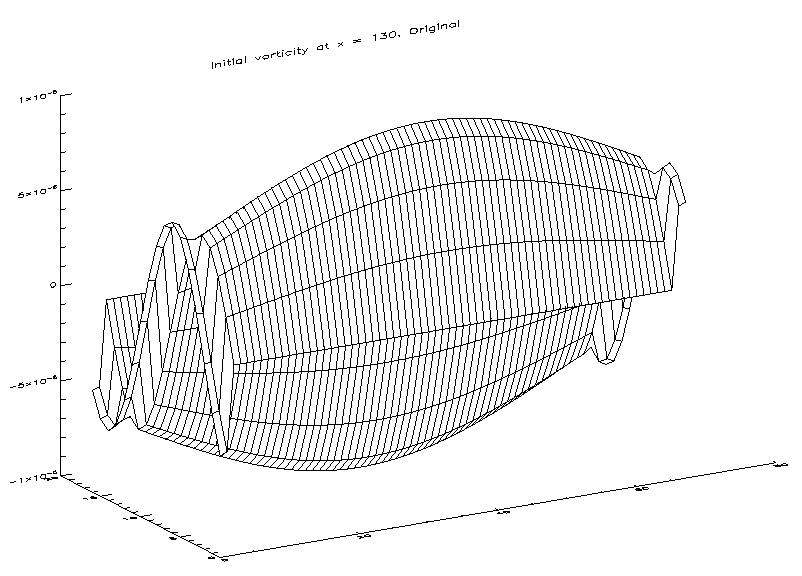
\includegraphics[width=0.48\textwidth,
keepaspectratio]{figs/init_noballoon.png}
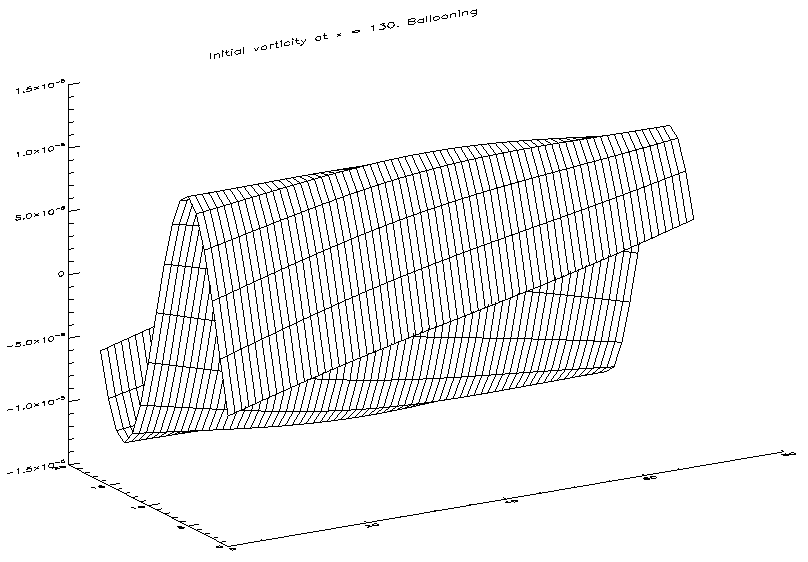
\includegraphics[width=0.48\textwidth, keepaspectratio]{figs/init_balloon.png}
\caption{Initial profiles in twist-shifted grid. {\bf Left}: Without ballooning 
transform, showing discontinuity at the matching location {\bf Right}: with 
ballooning transform}
%
\label{fig:ballooning}
%
\end{figure}
%
\note{The initial profiles code currently doesn't work very well for grids with
branch-cuts (e.g. divertor tokamak), and will often have jumps which then make
timesteps smaller}


\subsubsection{Expressions}
%
\label{sec:expressions}
%
\index{FieldFactory}
%
\index{function}
%
\index{Expressions}
%
If a more general function is needed, a variable can be initialised using the
\code{function} option for each variable. This overrides the original method
for that variable. e.g.
%
\begin{lstlisting}[language=bash,numbers=none]
[all]

xs_opt = 1  # Gaussian in X
ys_opt = 1  # Gaussian in Y
zs_opt = 2  # Sinusoidal in Z (axisymmetric direction)

[U]
scale = 1.0e-5

[p]
function = 1 + gauss(x-0.5)*gauss(y)*sin(z)
\end{lstlisting}
%
will use the original method to set $U$, but use the given expression to set
$p$.

Expressions can include the usual operators
(\code{+},\code{-},\code{*},\code{/}), including \code{\^} for exponents. The
following values are also already defined:
%
\begin{table}[htb!]
\centering
\caption{Initialisation expression values}
%
\label{tab:initexprvals}
%
\begin{tabular}{c | c }
\hline
Name & Description \\
\hline
x & $x$ position between $0$ and $1$ \\
y & $y$ position between $0$ and $2\pi$ (excluding the last point)\\
z & $z$ position between $0$ and $2\pi$ (excluding the last point)\\
pi & $3.1415\ldots$\\
\hline
\end{tabular}
%
\end{table}
%
By default, $x$ is defined as \code{i / (nx - 2*MXG)}, where \code{MXG} is the
width of the boundary region, by default 2. Hence $x$ actually goes from 0 on
the leftmost point to \code{(nx-1)/(nx-4)} on the rightmost point. This is not
a particularly good definition, but for most cases its sufficient to create
some initial profiles.
%
\index{Symmetric initial conditions}
%
For some problems like island reconnection simulations, it's useful to define
$x$ in a particular way which is more symmetric than the default. To do this,
set in BOUT.inp
%
\begin{lstlisting}[language=bash,numbers=none]
  [mesh]
  symmetricGlobalX = true
\end{lstlisting}
%
This will change the definition of $x$ to \code{i / (nx - 1)}, so $x$ is then
between $0$ and $1$ everywhere.

The functions in table~\ref{tab:initexprfunc} are also available in
expressions.
%
\begin{table}[htb!]
\centering
\caption{Initialisation expression functions}
%
\label{tab:initexprfunc}
%
\begin{tabular}{l | c }
\hline
Name & Description \\
\hline
abs(x) & Absolute value $\left|x\right|$\\
asin(x), acos(x), atan(x), atan(y,x) & Inverse trigonometric functions \\
ballooning(x) & Ballooning transform (eq~\ref{eq:ballooning_transform}, 
fig~\ref{fig:ballooning}) \\
ballooning(x,n) & Ballooning transform, using $n$ terms (default 3) \\
cos(x) & Cosine\\
cosh(x) & Hyperbolic cosine\\
exp(x) & Exponential \\
tanh(x) & Hyperbolic tangent \\
gauss(x) & Gaussian $\exp\left(-x^2/2\right) / \sqrt{2\pi}$\\
gauss(x, w) & Gaussian $\exp\left[-x^2/\left(2w^2\right)\right] / 
\left(w\sqrt{2\pi}\right)$\\
H(x) & Heaviside function: $1$ if $x > 0$ otherwise $0$\\
log(x) & Natural logarithm \\
max(x,y,...) & Maximum (variable arguments) \\
min(x,y,...) & Minimum (variable arguments) \\
mixmode(x) & A mixture of Fourier modes \\
mixmode(x, seed) & seed determines random phase (default 0.5) \\
power(x,y) & Exponent $x^y$ \\
sin(x) & Sine\\
sinh(x) & Hyperbolic sine\\
sqrt(x) & $\sqrt{x}$\\
tan(x) & Tangent \\
\hline
\end{tabular}
%
\end{table}
%
Note that to apply a ballooning transform in analytic expressions the
\texttt{ballooning} function should be used, and the global flag ``ballooning''
has no effect. There is an example code \texttt{test-ballooning} which compares
methods of setting initial conditions with ballooning transform.

The \texttt{mixmode(x)} function is a mixture of Fourier modes of the form:
%
\begin{align}
\mathrm{mixmode}\left(x\right) = \sum_{i=1}^{14} \frac{1}{\left(1 +
\left|i-4\right|\right)^2}\cos\left[ix + \phi\left(i,
\mathrm{seed}\right)\right]
\end{align}
%
where $\phi$ is a random phase between $-\pi$ and $+\pi$, which depends on the
seed. The factor in front of each term is chosen so that the 4th harmonic
($i=4$) has the highest amplitude. This is useful mainly for initialising
turbulence simulations, where a mixture of mode numbers is desired.
%
\index{variable initialisation}
%



\subsection{\texttt{FieldFactory} class}
%
This class provides a way to generate a field with a specified form. It
implements a recursive descent parser to turn a string containing something
like
%
\lstinline!"gauss(x-0.5,0.2)*gauss(y)*sin(3*z)"! into values in a
\lstinline!Field3D!
%
or
%
\lstinline!Field2D!
%
 object. Examples are given in the \texttt{test-fieldfactory} example:
%
\index{FieldFactory}
%
\begin{lstlisting}
FieldFactory f;
Field2D b = f.create2D("1 - x");
Field3D d = f.create3D("gauss(x-0.5,0.2)*gauss(y)*sin(z)");
\end{lstlisting}
%
This is done by creating a tree of
%
\lstinline!FieldGenerator!
%
 objects which then generate the field values:
%
\index{FieldGenerator}
%
\begin{lstlisting}[firstnumber=49]
class FieldGenerator {
 public:
  virtual ~FieldGenerator() { }
  virtual FieldGenerator* clone(const list<FieldGenerator*> args) {return NULL;}
  virtual BoutReal generate(int x, int y, int z) = 0;
};
\end{lstlisting}
%
All classes inheriting from
%
\lstinline!FieldGenerator!
%
 must implement a
%
\lstinline!generate!
%
 function, which returns the value at the given
%
\lstinline!(x,y,z)!
%
 position. Classes should also implement a
%
\lstinline!clone!
%
 function, which takes a list of arguments and creates a new instance of its
 class. This takes as input a list of other
%
\lstinline!FieldGenerator!
%
 objects, allowing a variable number of arguments.

The simplest generator is a fixed numerical value, which is represented by a
%
\lstinline!FieldValue!
%
 object:
%
\index{FieldValue}
%
\begin{lstlisting}[firstnumber=59]
class FieldValue : public FieldGenerator {
 public:
  FieldValue(BoutReal val) : value(val) {}
  BoutReal generate(int x, int y, int z) { return value; }
 private:
  BoutReal value;
};
\end{lstlisting}
%



\subsection{Adding a new function}
%
To add a new function to the FieldFactory, a new
%
\lstinline!FieldGenerator!
%
 class must be defined. Here we will use the example of the
%
\lstinline!sinh!
%
 function, implemented using a class
%
\lstinline!FieldSinh!
%
. This takes a single argument as input, but
%
\lstinline!FieldPI! takes no arguments, and \lstinline!FieldGaussian!
%
 takes either one or two.  Study these after reading this to see how these are
 handled.

First, edit \file{include/field\_factory.hxx} and add a class definition:
%
\begin{lstlisting}[firstnumber=122]
class FieldSinh : public FieldGenerator {
 public:
  FieldSinh(FieldGenerator* g) : gen(g) {}
  ~FieldSinh() {if(gen) delete gen;}

  FieldGenerator* clone(const list<FieldGenerator*> args);
  BoutReal generate(int x, int y, int z);
 private:
  FieldGenerator *gen;
};
\end{lstlisting}
%
The
%
\lstinline!gen!
%
 member is used to store the input argument, and to make sure it's deleted
 properly we add some code to the destructor. The constructor takes a single
 input, the
%
\lstinline!FieldGenerator! argument to the \lstinline!sinh! function, which is
stored in the member \lstinline!gen!
%
.

Next edit \file{src/field/field\_factory.cxx} and add the implementation of the
%
\lstinline!clone!
%
 and
%
\lstinline!generate!
%
 functions:
%
\begin{lstlisting}[firstnumber=100]
FieldGenerator* FieldSinh::clone(const list<FieldGenerator*> args) {
  if(args.size() != 1) {
    output << "FieldFactory error: Incorrect number of arguments to sinh 
function. Expecting 1, got " << args.size() << endl;
    return NULL;
  }

  return new FieldSinh(args.front());
}

BoutReal FieldSinh::generate(int x, int y, int z) {
  return sinh(gen->generate(x,y,z));
}
\end{lstlisting}
%
The
%
\lstinline!clone! function first checks the number of arguments using
\lstinline!args.size()!
%
. This is used in
%
\lstinline!FieldGaussian!
%
 to handle different numbers of input, but in this case we print an error
 message and return
%
\lstinline!NULL! if the number of inputs isn't one. \lstinline!clone!
%
 then creates a new
%
\lstinline!FieldSinh! object, passing the first argument
(\lstinline!args.front()!
%
) to the constructor (which then gets stored in the
%
\lstinline!gen!
%
 member variable).

The
%
\lstinline!generate! function for \lstinline!sinh!
%
 just gets the value of the input by calling
%
\lstinline!gen->generate(x,y,z)!, calculates \lstinline!sinh!
%
 of it and returns the result.

The
%
\lstinline!clone! function means that the parsing code can make copies of any
\lstinline!FieldGenerator!
%
 class if it's given a single instance to start with. The final step is
 therefore to give the
%
\lstinline!FieldFactory!
%
class an instance of this new generator. Edit the
%
\lstinline!FieldFactory! constructor \lstinline!FieldFactory::FieldFactory()!
%
 in \file{src/field/field\_factory.cxx} and add the line:
%
\begin{lstlisting}[firstnumber=196]
addGenerator("sinh", new FieldSinh(NULL));
\end{lstlisting}
%
That's it! This line associates the string
%
\lstinline!"sinh"! with a \lstinline!FieldGenerator!
%
. Even though
%
\lstinline!FieldFactory! doesn't know what type of \lstinline!FieldGenerator!
%
 it is, it can make more copies by calling the
%
\lstinline!clone!
%
 member function. This is a useful technique for polymorphic objects in C++
 called the ``Virtual Constructor'' idiom.



\subsection{Parser internals}
%
When a
%
\lstinline!FieldGenerator! is added using the \lstinline!addGenerator!
%
 function, it is entered into a
%
\lstinline!std::map! which maps strings to \lstinline!FieldGenerator!
%
objects (\file{include/field\_factory.hxx}):

%
\begin{lstlisting}[firstnumber=223]
map<string, FieldGenerator*> gen;
\end{lstlisting}
%
Parsing a string into a tree of
%
\lstinline!FieldGenerator!
%
 objects is done by first splitting the string up into separate tokens like
 operators like '*', brackets '(', names like 'sinh' and so on, then
 recognising patterns in the stream of tokens. Recognising tokens is done in
 \file{src/field/field\_factory.cxx}:
%
\begin{lstlisting}[firstnumber=259]
char FieldFactory::nextToken() {
 ...
\end{lstlisting}
%
This returns the next token, and setting the variable
%
\lstinline!char curtok!
%
 to the same value.  This can be one of:
%
\begin{itemize}
\item -1 if the next token is a number. The variable
%
\lstinline!BoutReal curval!
%
 is set to the value of the token
\item -2 for a string (e.g. ``sinh'', ``x'' or ``pi''). This includes anything 
which starts with a letter, and
  contains only letters, numbers, and underscores. The string is stored in the
  variable
%
\lstinline!string curident!
%
.
\item 0 to mean end of input
\item The character if none of the above. Since letters and numbers are taken
    care of (see above), this includes brackets and operators like '+' and '-'.
\end{itemize}
%
The parsing stage turns these tokens into a tree of
%
\lstinline!FieldGenerator!
%
 objects, starting with the
%
\lstinline!parse()!
%
 function
%
\begin{lstlisting}[firstnumber=484]
FieldGenerator* FieldFactory::parse(const string &input) {
   ...
\end{lstlisting}
%
which puts the input string into a stream so that
%
\lstinline!nextToken()!
%
 can use it, then calls the
%
\lstinline!parseExpression()!
%
 function to do the actual parsing:
%
\begin{lstlisting}[firstnumber=477]
FieldGenerator* FieldFactory::parseExpression() {
   ...
\end{lstlisting}
%
This breaks down expressions in stages, starting with writing every expression
as
%
\begin{verbatim}
expression := primary [ op primary ]
\end{verbatim}
%
i.e. a primary expression, and optionally an operator and another primary
expression. Primary expressions are handled by the
%
\lstinline!parsePrimary()! function, so first \lstinline!parsePrimary()!
%
 is called, and then
%
\lstinline!parseBinOpRHS! which checks if there is an operator, and if so calls
\lstinline!parsePrimary()!
%
 to parse it. This code also takes care of operator precedence by keeping track
 of the precedence of the current operator. Primary expressions are then
 further broken down and can consist of either a number, a name (identifier), a
 minus sign and a primary expression, or brackets around an  expression:
%
\begin{verbatim}
primary := number
        := identifier
        := '-' primary
        := '(' expression ')'
        := '[' expression ']'
\end{verbatim}
%
The minus sign case is needed to handle the unary minus e.g.
%
\lstinline!"-x"!
%
. Identifiers are handled in
%
\lstinline!parseIdentifierExpr()!
%
 which handles either variable names, or functions
%
\begin{verbatim}
identifier := name
           := name '(' expression [ ',' expression [ ',' ... ] ] ')'
\end{verbatim}
%
i.e. a name, optionally followed by brackets containing one or more expressions
separated by commas.  names without brackets are treated the same as those with
empty brackets, so
%
\lstinline!"x"!
%
 is the same as
%
\lstinline!"x()"!. A list of inputs (\lstinline!list<FieldGenerator*> args;!
%
) is created, the
%
\lstinline!gen! map is searched to find the \lstinline!FieldGenerator!
%
 object corresponding to the name, and the list of inputs is passed to the
 object's
%
\lstinline!clone!
%
 function.





\section{Implementation}
%
\index{Options}
%
To control the behaviour of BOUT++ a set of options is used, with options
organised into sections which can be nested. To represent this tree structure
there is the
%
\lstinline!Options!
%
 class defined in \file{bout++/include/options.hxx}
%
\begin{lstlisting}
class Options {
 public:
  // Setting options
  void set(const string &key,const int &val,const string &source="");
  ...
  // Testing if set
  bool isSet(const string &key);
  // Getting options
  void get(const string &key,int &val,const int &def,bool log=true);
  ...
  // Get a subsection. Creates if doesn't exist
  Options* getSection(const string &name);
};
\end{lstlisting}
%
To access the options, there is a static function (singleton)
%
\begin{lstlisting}
  Options *options = Options::getRoot();
\end{lstlisting}
%
which gives the top-level (root) options class. Setting options is done using
the
%
\lstinline!set()!
%
 methods which are currently defined for
%
\lstinline!int!, \lstinline!BoutReal!, \lstinline!bool!
%
 and
%
\lstinline!string!
%
. For example:
%
\begin{lstlisting}
  options->set("nout", 10);      // Set an integer
  options->set("restart", true); // A bool
\end{lstlisting}
%
Often it's useful to see where an option setting has come from e.g. the name of
the options file or ``command line''. To specify a source, pass it as a third
argument:
%
\begin{lstlisting}
  options->set("nout", 10, "manual");
\end{lstlisting}
%
To create a section, just use
%
\lstinline!getSection!
%
: if it doesn't exist it will be created.
%
\begin{lstlisting}
  Options *section = options->getSection("mysection");
  section->set("myswitch", true);
\end{lstlisting}
%
To get options, use the
%
\lstinline!get()!
%
 method which take the name of the option, the variable to set, and the default
 value.
%
\begin{lstlisting}
  int nout;
  options->get("nout", nout, 1);
\end{lstlisting}
%
Internally,
%
\lstinline!Options!
%
 converts all types to strings and does type conversion when needed, so the
 following code would work:
%
\begin{lstlisting}
  Options *options = Options::getRoot();
  options->set("test", "123");
  int val;
  options->get("test", val, 1);
\end{lstlisting}
%
This is because often the type of the option is not known at the time when it's
set, but only when it's requested.

By default, the
%
\lstinline!get!
%
 methods output a message to the log files giving the value used and the source
 of that value.  To suppress this, set the
%
\lstinline!log! argument to \lstinline!false!
%
:
%
\begin{lstlisting}
  options->get("test", val, 1, false);
\end{lstlisting}
%



\subsection{Reading options}
%
To allow different input file formats, each file parser implements the
%
\lstinline!OptionParser!
%
 interface defined in \file{bout++/src/sys/options/optionparser.hxx}
%
\index{OptionParser}
%
\begin{lstlisting}
class OptionParser {
 public:
  virtual void read(Options *options, const string &filename) = 0;
 private:
};
\end{lstlisting}
%
and so just needs to implement a single function which reads a given file name
and inserts the options into the given
%
\lstinline!Options!
%
object.

To use these parsers and read in a file, there is the
%
\lstinline!OptionsReader!
%
 class defined in \file{bout++/include/optionsreader.hxx}
%
\index{OptionsReader}
%
\begin{lstlisting}
class OptionsReader {
 public:
 void read(Options *options, const char *file, ...);
 void parseCommandLine(Options *options, int argc, char **argv);
};
\end{lstlisting}
%
This is a singleton object which is accessed using
%
\begin{lstlisting}
  OptionsReader *reader = OptionsReader::getInstance();
\end{lstlisting}
%
so to read a file \file{BOUT.inp} in a directory given in a variable
%
\lstinline!data_dir!
%
 the following code is used in \file{bout++.cxx}:
%
\begin{lstlisting}
  Options *options = Options::getRoot();
  OptionsReader *reader = OptionsReader::getInstance();
  reader->read(options, "%s/BOUT.inp", data_dir);
\end{lstlisting}
%
To parse command line arguments as options, the
%
\lstinline!OptionsReader!
%
class has a method:
%
\begin{lstlisting}
  reader->parseCommandLine(options, argc, argv);
\end{lstlisting}
%
This is currently quite rudimentary and needs improving.

%%%%%%%%%%%%%%%%%%%%%%%%%%%%%%%%%%%%%%%%%%%%%%%%%%%%%%%%%%%%%%%%%%%





\section{Time integration}
%



\subsection{Options}
%
\label{sec:timeoptions}
%
\index{time integration}
%
BOUT++ can be compiled with several different time-integration solvers
% 2015.02.17 loeiten: commented this as the section does not exist
%(see section~\ref{sec:solverlibrary})
, and at minimum should have Runge-Kutta (RK4) and PVODE (BDF/Adams) solvers
available.

The solver library used is set using the \code{solver:type} option, so either
in BOUT.inp:
%
\begin{lstlisting}[language=bash,numbers=none]
[solver]
type = rk4  # Set the solver to use
\end{lstlisting}
%
or on the command line by adding \code{solver:type=pvode} for example:
%
\begin{lstlisting}[language=bash,numbers=none]
mpirun -np 4 ./2fluid solver:type=rk4
\end{lstlisting}
%
{\bf NB}: Make sure there are no spaces around the ``='' sign:
\code{solver:type =pvode} won't work (probably).  Table~\ref{tab:solvers} gives
a list of time integration solvers, along with any compile-time options needed
to make the solver available.
%
\begin{table}[htb!]
\centering
\caption{Available time integration solvers}
%
\label{tab:solvers}
%
\begin{tabular}{c | c | c}
\hline
Name & Description & Compile options \\
\hline
euler & Euler explicit method & Always available \\
rk4 & Runge-Kutta 4th-order explicit method & Always available \\
karniadakis & Karniadakis explicit method & Always available \\
pvode & 1998 PVODE with BDF method & Always available \\
cvode & SUNDIALS CVODE. BDF and Adams methods & --with-cvode \\
ida & SUNDIALS IDA. DAE solver & --with-ida \\
petsc & PETSc TS methods & --with-petsc \\
\hline
\end{tabular}
%
\end{table}
%
Each solver can have its own settings which work in slightly different ways,
but some common settings and which solvers they are used in are given in
table~\ref{tab:solveropts}.
%
\begin{table}[htb!]
\centering
\caption{Time integration solver options}
%
\label{tab:solveropts}
%
\begin{tabular}{c | c | c}
\hline
Option & Description & Solvers used \\
\hline
atol & Absolute tolerance & rk4, pvode, cvode, ida \\
rtol & Relative tolerance & rk4, pvode, cvode, ida \\
mxstep & Maximum internal steps  & rk4 \\
       & per output step & \\
max\_timestep & Maximum timestep & rk4, cvode \\
timestep & Starting timestep & rk4, karniadakis, euler \\
adaptive & Adapt timestep? (Y/N) & rk4 \\
use\_precon & Use a preconditioner? (Y/N) & pvode, cvode, ida \\
mudq, mldq & BBD preconditioner settings & pvode, cvode, ida \\
mukeep, mlkeep & & \\
maxl & & \\
use\_jacobian & Use user-supplied Jacobian? (Y/N) & cvode \\
adams\_moulton & Use Adams-Moulton method & cvode \\
 & rather than BDF & \\
diagnose & Collect and print additional diagnostics & cvode \\
\hline
\end{tabular}
%
\end{table}
%
The most commonly changed options are the  absolute and relative solver
tolerances, \code{ATOL} and \code{RTOL} which should be varied to check
convergence.



\subsection{ODE integration}
%
The Solver class can be used to solve systems of ODEs inside a physics model:
Multiple Solver objects can exist besides the main one used for time
integration.  Example code is in \file{examples/test-integrate}.

To use this feature, systems of ODEs must be represented by a class derived
from \code{PhysicsModel} (see section~\ref{sec:newapi}).

%
\begin{lstlisting}
class MyFunction : public PhysicsModel {
 public:
  int init(bool restarting) {
    // Initialise ODE
    // Add variables to solver as usual
    solver->add(result, "result");
    ...
  }

  int rhs(BoutReal time) {
    // Specify derivatives of fields as usual
    ddt(result) = ...
  }
 private:
  Field3D result;
};
\end{lstlisting}
%
To solve this ODE, create a new Solver object:
%
\begin{lstlisting}[numbers=none]
Solver* ode = Solver::create(Options::getRoot()->getSection("ode"));
\end{lstlisting}
%
This will look in the section \texttt{[ode]} in the options file.  {\bf
Important:} To prevent this solver overwriting the main restart files with its
own restart files, either disable restart files:
%
\begin{lstlisting}[numbers=none]
[ode]
enablerestart = false
\end{lstlisting}
%
or specify a different directory to put the restart files:
%
\begin{lstlisting}[numbers=none]
[ode]
restartdir = ode  # Restart files ode/BOUT.restart.0.nc, ...
\end{lstlisting}
%
Create a model object, and pass it to the solver:
%
\begin{lstlisting}[numbers=none]
MyFunction* model = new MyFunction();
ode->setModel(model);
\end{lstlisting}
%
Finally tell the solver to perform the integration:
%
\begin{lstlisting}[numbers=none]
ode->solve(5, 0.1);
\end{lstlisting}
%
The first argument is the number of steps to take, and the second is the size
of each step. These can also be specified in the options, so calling
%
\begin{lstlisting}[numbers=none]
ode->solve();
\end{lstlisting}
%
will cause ode to look in the input for \texttt{nout} and \texttt{timestep}
options:
%
\begin{lstlisting}[numbers=none]
[ode]
nout = 5
timestep = 0.1
\end{lstlisting}
%
Finally, delete the model and solver when finished:
%
\begin{lstlisting}[numbers=none]
delete model;
delete solver;
\end{lstlisting}
%
{\bf Note: } If an ODE needs to be solved multiple times, at the moment it is
recommended to delete the solver, and create a new one each time.



\subsection{Preconditioning}
%
At every time step, an implicit scheme such as BDF has to solve a non-linear
problem to find the next solution. This is usually done using Newton's method,
each step of which involves solving a linear (matrix) problem. For $N$ evolving
variables is an $N\times N$ matrix and so can be very large.  By default
matrix-free methods are used, in which the Jacobian $\mathcal{J}$ is
approximated by finite differences (see next subsection), and so this matrix
never needs to be explicitly calculated. Finding a solution to this matrix can
still be difficult, particularly as $\delta t$ gets large compared with some
time-scales in the system (i.e. a stiff problem).

A preconditioner is a function which quickly finds an approximate solution to
this matrix, speeding up convergence to a solution. A preconditioner does not
need to include all the terms in the problem being solved, as the
preconditioner only affects the convergence rate and not the final solution. A
good preconditioner can therefore concentrate on solving the parts of the
problem with the fastest time-scales.

A simple example\footnote{Taken from a talk by L.Chacon available here
\url{https://bout.llnl.gov/pdf/workshops/2011/talks/Chacon_bout2011.pdf}} is a
coupled wave equation, solved in the \texttt{test-precon} example code:
%
\begin{align}
\frac{\partial u}{\partial t} = \partial_{||}v \qquad \frac{\partial
v}{\partial t} = \partial_{||} u
\end{align}
%
First, calculate the Jacobian of this set of equations by taking partial
derivatives of the time-derivatives with respect to each of the evolving
variables
%
\begin{align}
\mathcal{J} = \left(%
\begin{array}{cc}
\frac{\partial}{\partial u}\frac{\partial u}{\partial t} & 
\frac{\partial}{\partial v}\frac{\partial u}{\partial t}\\
\frac{\partial}{\partial u}\frac{\partial v}{\partial t} & 
\frac{\partial}{\partial v}\frac{\partial v}{\partial t}
\end{array}
%
\right) = \left(%
\begin{array}{cc}
0 & \partial_{||} \\
\partial_{||} & 0
\end{array}
%
\right)
\end{align}
%
In this case $\frac{\partial u}{\partial t}$ doesn't depend on $u$ nor
$\frac{\partial v}{\partial t}$ on $v$, so the diagonal is empty. Since the
equations are linear, the Jacobian doesn't depend on $u$ or $v$ and so
%
\begin{align}
\frac{\partial}{\partial t}\left(%
\begin{array}{c}
u \\
v
\end{array}\right) = \mathcal{J}
%
 \left(%
\begin{array}{c}
u \\
v
\end{array}
%
\right)
\end{align}
%
In general for non-linear functions $\mathcal{J}$ gives the change in
time-derivatives in response to changes in the state variables $u$ and $v$.

In implicit time stepping, the preconditioner needs to solve an equation
%
\begin{align}
\mathcal{I} - \gamma \mathcal{J}
\end{align}
%
where $\mathcal{I}$ is the identity matrix, and $\gamma$ depends on the time
step and method (e.g. $\gamma = \delta t^2$ for backwards Euler method). For
the simple wave equation problem, this is
%
\begin{align}
\mathcal{I} - \gamma \mathcal{J} = \left(%
\begin{array}{cc}
1 & -\gamma\partial_{||} \\
-\gamma\partial_{||} & 1
\end{array}
%
\right)
\end{align}
%
This matrix can be block inverted using Schur factorisation\footnote{See paper
\url{http://arxiv.org/abs/1209.2054} for an application to 2-fluid equations}
%
\begin{align}
\left(%
\begin{array}{cc}
  \bb{E} & \bb{U} \\
  \bb{L} & \bb{D}
\end{array}\right)^{-1}
%
 = \left(%
\begin{array}{cc}
  \bb{I} & -\bb{E}^{-1}\bb{U} \\
  0 & \bb{I}
\end{array}
%
\right)\left(%
\begin{array}{cc}
  \bb{E}^{-1} & 0 \\
  0 & \bb{P}_{Schur}^{-1}
\end{array}
%
\right)\left(%
\begin{array}{cc}
  \bb{I} & 0 \\
  -\bb{L}\bb{E}^{-1} & \bb{I}
\end{array}
%
\right)
\end{align}
%
where $\bb{P}_{Schur} = \bb{D} - \bb{L}\bb{E}^{-1}\bb{U}$ Using this, the wave
problem becomes:
%
\begin{align}
\left(%
\begin{array}{cc}
1 & -\gamma\partial_{||} \\
-\gamma\partial_{||} & 1
\end{array}\right)^{-1}
%
 = \left(%
\begin{array}{cc}
1 & \gamma\partial_{||} \\
0 & 1
\end{array}
%
\right)\left(%
\begin{array}{cc}
1 & 0 \\
0 & \left(1 - \gamma^2\partial^2_{||}\right)^{-1}
\end{array}
%
\right)\left(%
\begin{array}{cc}
1 & 0 \\
\gamma\partial_{||} & 1
\end{array}
%
\right)
%
\label{eq:precon}
%
\end{align}
%
The preconditioner is implemented by defining a function of the form
%
\begin{lstlisting}[numbers=none]
int precon(BoutReal t, BoutReal gamma, BoutReal delta) {
  ...
}
\end{lstlisting}
%
which takes as input the current time, the $\gamma$ factor appearing above, and
$\delta$ which is only important for constrained problems (not discussed
here... yet). The current state of the system is stored in the state variables
(here
%
\lstinline!u! and \lstinline!v!
%
), whilst the vector to be preconditioned is stored in the time derivatives
(here
%
\lstinline!ddt(u)! and \lstinline!ddt(v)!
%
). At the end of the preconditioner the result should be in the time
derivatives. A preconditioner which is just the identity matrix and so does
nothing is therefore:
%
\begin{lstlisting}[numbers=none]
int precon(BoutReal t, BoutReal gamma, BoutReal delta) {
}
\end{lstlisting}
%
\note{This changed in github/bendudson on 15th Aug 2014. In older versions the
result must be returned in the state variables}

To implement the preconditioner in equation~\ref{eq:precon}, first apply the
rightmost matrix to the given vector:
%
\begin{align}
\left(%
\begin{array}{c}
\texttt{ddt(u)} \\
\texttt{ddt(v)}
\end{array}
%
\right) = \left(%
\begin{array}{cc}
1 & 0 \\
\gamma\partial_{||} & 1
\end{array}
%
\right)\left(%
\begin{array}{c}
\texttt{ddt(u)} \\
\texttt{ddt(v)}
\end{array}
%
\right)
\end{align}
%
\begin{lstlisting}[numbers=none]
int precon(BoutReal t, BoutReal gamma, BoutReal delta) {
  mesh->communicate(ddt(u));
  //ddt(u) = ddt(u);
  ddt(v) = gamma*Grad_par(ddt(u)) + ddt(v);
\end{lstlisting}
%
note that since the preconditioner is linear, it doesn't depend on $u$ or $v$.
As in the RHS function, since we are taking a differential of \texttt{ddt(u)},
it first needs to be communicated to exchange guard cell values.

The second matrix
%
\begin{align}
\left(%
\begin{array}{c}
\texttt{ddt(u)} \\
\texttt{ddt(v)}
\end{array}
%
\right) \leftarrow \left(%
\begin{array}{cc}
1 & 0 \\
0 & \left(1 - \gamma^2\partial^2_{||}\right)^{-1}
\end{array}
%
\right)\left(%
\begin{array}{c}
\texttt{ddt(u)} \\
\texttt{ddt(v)}
\end{array}
%
\right)
\end{align}
%
doesn't alter $u$, but solves a parabolic equation in the parallel direction.
There is a solver class to do this called \texttt{InvertPar} which solves the
equation $\left(A + B\partial_{||}^2\right)x = b$ where $A$ and $B$ are
%
\lstinline!Field2D! or constants\footnote{This \texttt{InvertPar} class can
handle cases with closed field-lines and twist-shift boundary conditions for
tokamak simulations}. In \lstinline!physics_init!
%
 we create one of these solvers:
%
\begin{lstlisting}[numbers=none]
InvertPar *inv; // Parallel inversion class
int physics_init(bool restarting) {
   ...
   inv = InvertPar::Create();
   inv->setCoefA(1.0);
   ...
}
\end{lstlisting}
%
In the preconditioner we then use this solver to update $v$:
%
\begin{lstlisting}[numbers=none]
  inv->setCoefB(-SQ(gamma));
  ddt(v) = inv->solve(ddt(v));
\end{lstlisting}
%
which solves $ddt(v) \leftarrow \left(1 - \gamma^2\partial_{||}^2\right)^{-1}
ddt(v)$.  The final matrix just updates $u$ using this new solution for $v$
%
\begin{align}
\left(%
\begin{array}{c}
\texttt{ddt(u)} \\
\texttt{ddt(v)}
\end{array}
%
\right) \leftarrow \left(%
\begin{array}{cc}
1 & \gamma\partial_{||} \\
0 & 1
\end{array}
%
\right)\left(%
\begin{array}{c}
\texttt{ddt(u)} \\
\texttt{ddt(v)}
\end{array}
%
\right)
\end{align}
%
\begin{lstlisting}[numbers=none]
  mesh->communicate(ddt(v));
  ddt(u) = ddt(u) + gamma*Grad_par(ddt(v));
\end{lstlisting}
%
Finally, boundary conditions need to be imposed, which should be consistent
with the conditions used in the RHS
%
\begin{lstlisting}[numbers=none]
  ddt(u).applyBoundary("dirichlet");
  ddt(v).applyBoundary("dirichlet");
\end{lstlisting}
%
To use the preconditioner, pass the function to the solver in
%
\lstinline!physics_init!
%
\begin{lstlisting}
int physics_init(bool restarting) {
  solver->setPrecon(precon);
  ...
}
\end{lstlisting}
%
then in the \texttt{BOUT.inp} settings file switch on the preconditioner
%
\begin{lstlisting}[language=bash,numbers=none]
[solver]
type = cvode          # Need CVODE or PETSc
use_precon = true     # Use preconditioner
rightprec = false     # Use Right preconditioner (default left)
\end{lstlisting}
%



\subsection{Jacobian function}
%



\subsection{DAE constraint equations}
%
Using the IDA solver, BOUT++ can solve Differential Algebraic Equations (DAEs),
in which algebraic constraints are used for some variables.



\subsection{Monitoring the simulation output}
%
Monitoring of the solution can be done at two levels: output monitoring, and
timestep monitoring. Output monitoring occurs only when data is written to
file, whereas timestep monitoring is every timestep and so (usually) much more
frequent. Examples of both are in \file{examples/monitor} and
\file{examples/monitor-newapi}.

{\bf Output monitoring}: At every output timestep the solver calls a monitor
function, which writes the output dump file, calculates and prints timing
information and estimated time remaining. If you want to run additional code or
write data to a different file, you can add monitor function(s).

You can call your output monitor function whatever you like, but it must have 4
inputs and return an int:
%
\begin{lstlisting}
int my_output_monitor(Solver *solver, BoutReal simtime, int iter, int NOUT) {
  ...
}
\end{lstlisting}
%
The first input is the solver object, the second is the current simulation
time, the third is the output number, and the last is the total number of
outputs requested. To get the solver to call this function every output time,
put in your
%
\lstinline!physics_init!
%
 code:
%
\begin{lstlisting}
  solver->addMonitor(my_output_monitor);
\end{lstlisting}
%
If you want to later remove a monitor, you can do so with
%
\begin{lstlisting}
  solver->removeMonitor(my_output_monitor);
\end{lstlisting}
%
A simple example using this monitor is:
%
\begin{lstlisting}
int my_output_monitor(Solver *solver, BoutReal simtime, int iter, int NOUT) {
  output.write("My monitor, time = %e, dt = %e\n",
      simtime, solver->getCurrentTimestep());
}

int physics_init(bool restarting) {
  solver->addMonitor(my_monitor);
}
\end{lstlisting}
%
See the monitor example (\file{examples/monitor}) for full code.


{\bf Timestep monitoring}: This works in the same way as output monitoring.
First define a monitor function:
%
\begin{lstlisting}
int my_timestep_monitor(Solver *solver, BoutReal simtime, BoutReal lastdt) {
  ...
}
\end{lstlisting}
%
where
%
\lstinline!simtime! will again contain the current simulation time, and
\lstinline!lastdt!
%
 the last timestep taken. Add this function to the solver:
%
\begin{lstlisting}
  solver->addTimestepMonitor(my_timestep_monitor);
\end{lstlisting}
%
Timestep monitoring is disabled by default, unlike output monitoring. To enable
timestep monitoring, set in the options file (BOUT.inp):
%
\begin{lstlisting}
[solver]
monitor_timestep = true
\end{lstlisting}
%
or put on the command line
%
\lstinline!solver:monitor_timestep=true!
%
. When this is enabled, it will change how solvers like CVODE and PVODE (the
default solvers) are used. Rather than being run in NORMAL mode, they will
instead be run in SINGLE\_STEP mode (see the SUNDIALS notes
here:\url{http://computation.llnl.gov/casc/sundials/support/notes.html}). This
may in some cases be less efficient.

%%%%%%%%%%%%%%%%%%%%%%%%%%%%%%%%%%%%%%%%%%%%%%%%%%%%%%%%%%%%%%%%%%%





\section{Boundary conditions}
%
\label{sec:bndryopts}
%
\index{boundary conditions}
%
\note{The boundary conditions are currently not set in the corner cells.
Therefore: When using stecils which uses corner cells (like the Arakawa scheme)
care must be taken, and the boundary conditions in the corner cells must be set
manually.}

Like the variable initialisation, boundary conditions can be set for each
variable in individual sections, with default values in a section \code{[All]}.
Boundary conditions are specified for each variable, being applied to variable
itself during initialisation, and the time-derivatives at each timestep. They
are a combination of a basic boundary condition, and optional modifiers.

When finding the boundary condition for a variable \code{var} on a boundary
region, the options are checked in order from most to least specific:
%
\begin{itemize}
\item Section \code{var}, \code{bndry\_} + region name. Depending on the mesh
    file, regions of the grid are given labels. Currently these are
    \code{core}, \code{sol}, \code{pf} and \code{target} which are intended for
    tokamak edge simulations. Hence the variables checked are
    \code{bndry\_core}, \code{bndry\_pf} etc.
\item Section \code{var}, \code{bndry\_} + boundary side. These names are
  \code{xin}, \code{xout}, \code{yup} and \code{ydown}.
\item Section \code{var}, variable \code{bndry\_all}
\item The same settings again except in section \code{All}.
\end{itemize}
%
The default setting for everything is therefore \code{bndry\_all} in the
\code{All} section.

Boundary conditions are given names, with optional arguments in brackets.
Currently implemented boundary conditions are:
%
\begin{itemize}
\item \code{dirichlet} - Set to zero
\item \code{dirichlet(<number>)} - Set to some number e.g. \code{dirichlet(1)}
    sets the boundary to $1.0$
\item \code{neumann} - Zero gradient
\item \code{robin} - A combination of zero-gradient and zero-value $a f +
    b\deriv{f}{x} = g$ where the syntax is \code{robin(a, b, g)}.
\item \code{constgradient} - Constant gradient across boundary

\item \code{zerolaplace} - Laplacian = 0, decaying solution (X boundaries only)
\item \code{zerolaplace2} - Laplacian = 0, using coefficients from the
    Laplacian inversion and Delp2 operator.
\item \code{constlaplace} - Laplacian = const, decaying solution (X boundaries 
only)
\end{itemize}
%
The zero- or constant-Laplacian boundary conditions works as follows:
%
\begin{align*}
\nabla_\perp^2 f =& 0 \\ &\simeq& g^{xx}\frac{\partial^2 f}{\partial x^2} +
    g^{zz}\frac{\partial^2 f}{\partial z^2}
\end{align*}
%
which when Fourier transformed in $z$ becomes:
%
\begin{align}
g^{xx}\frac{\partial^2 \hat{f}}{\partial x^2} - g^{zz}k_z^2 \hat{f} = 0
\end{align}
%
which has the solution
%
\begin{align}
\hat{f} = Ae^{xk_z\sqrt{g^{zz}/g^{xx}}} + Be^{-xk_z\sqrt{g^{zz}/g^{xx}}}
\end{align}
%
Assuming that the solution should decay away from the domain, on the inner $x$
boundary $B = 0$, and on the outer boundary $A = 0$.
%
\index{Boundary modifiers}
%
Boundary modifiers change the behaviour of boundary conditions, and more than
one modifier can be used. Currently the following are available:
%
\begin{itemize}
\item \code{relax} - Relaxing boundaries. Evolve the variable towards the given
    boundary condition at a given rate
\item \code{shifted} - Apply boundary conditions in orthogonal X-Z coordinates, 
rather than
  field-aligned
\item \code{width} - Modifies the width of the region over which the boundary 
condition is applied
\end{itemize}
%
These are described in the following subsections.



\subsection{Relaxing boundaries}
%
All boundaries can be modified to be ``relaxing'' which are a combination of
zero-gradient time-derivative, and whatever boundary condition they are applied
to. The idea is that this prevents sharp discontinuities at boundaries during
transients, whilst maintaining the desired boundary condition on longer
time-scales. In some cases this can improve the numerical stability and
timestep.

For example, \code{relax(dirichlet)} will make a field $f$ at point $i$ in the
boundary follow a point $i-1$ in the domain:
%
\begin{align}
\left.\deriv{f}{t}\right|_i = \left.\deriv{f}{t}\right|_{i-1}  - f_i / \tau
\end{align}
%
where $\tau$ is a time-scale for the boundary (currently set to 0.1, but will
be a global option).  When the time-derivatives are slow close to the boundary,
the boundary relaxes to the desired condition (Dirichlet in this case), but
when the time-derivatives are large then the boundary approaches Neumann to
reduce discontinuities.

By default, the relaxation rate is set to $10$ (i.e. a time-scale of
$\tau=0.1$).  To change this, give the rate as the second argument e.g.
\code{relax(dirichlet, 2)} would relax to a Dirichlet boundary condition at a
rate of $2$.



\subsection{Shifted boundaries}
%
By default boundary conditions are applied in field-aligned coordinates, where
$y$ is along field-lines but $x$ has a discontinuity at the twist-shift
location. If radial derivatives are being done in shifted coordinates where $x$
and $z$ are orthogonal, then boundary conditions should also be applied in
shifted coordinates. To do this, the \code{shifted} boundary modifier applies a
$z$ shift, applies the boundary condition, then shifts back. For example:
%
\begin{lstlisting}[numbers=none]
bndry_core = shifted( neumann )
\end{lstlisting}
%
would ensure that radial derivatives were zero in shifted coordinates on the
core boundary.



\subsection{Changing the width of boundaries}
%
To change the width of a boundary region, the \code{width} modifier changes the
width of a boundary region before applying the boundary condition, then changes
the width back afterwards. To use, specify the boundary condition and the
width, for example
%
\begin{lstlisting}[numbers=none]
bndry_core = width( neumann , 4 )
\end{lstlisting}
%
would apply a Neumann boundary condition on the innermost 4 cells in the core,
rather than the usual 2.  When combining with other boundary modifiers, this
should be applied first e.g.
%
\begin{lstlisting}[numbers=none]
bndry_sol = width( relax( dirichlet ), 3)
\end{lstlisting}
%
would relax the last 3 cells towards zero, whereas
%
\begin{lstlisting}[numbers=none]
bndry_sol = relax( width( dirichlet, 3) )
\end{lstlisting}
%
would only apply to the usual 2, since relax didn't use the updated width.

Limitations:
%
\begin{enumerate}
  \item Because it modifies then restores a globally-used BoundaryRegion, this
      code is not thread safe.

  \item Boundary conditions can't be applied across processors, and no checks
      are done that the width asked for fits within a single processor.
\end{enumerate}
%



\subsection{Examples}
%
This example is taken from the UEDGE benchmark test (in
\texttt{examples/uedge-benchmark}):
%
\begin{lstlisting}[language=bash,numbers=none]
[All]
bndry_all = neumann # Default for all variables, boundaries

[Ni]
bndry_target = neumann
bndry_core = relax(dirichlet(1.))   # 1e13 cm^-3 on core boundary
bndry_all  = relax(dirichlet(0.1))  # 1e12 cm^-3 on other boundaries

[Vi]
bndry_ydown = relax(dirichlet(-1.41648))   # -3.095e4/Vi_x
bndry_yup   = relax(dirichlet( 1.41648))
\end{lstlisting}
%
The variable \code{Ni} (density) is set to a Neumann boundary condition on the
targets (yup and ydown), relaxes towards $1$ on the core boundary, and relaxes
to $0.1$ on all other boundaries. Note that the \code{bndry\_target = neumann}
needs to be in the \code{Ni} section: If we just had
%
\begin{lstlisting}[language=bash,numbers=none]
[All]
bndry_all = neumann # Default for all variables, boundaries

[Ni]
bndry_core = relax(dirichlet(1.))   # 1e13 cm^-3 on core boundary
bndry_all  = relax(dirichlet(0.1))  # 1e12 cm^-3 on other boundaries
\end{lstlisting}
%
then the ``target'' boundary condition for \code{Ni} would first search in the
\code{[Ni]} section for \code{bndry\_target}, then for \code{bndry\_all} in the
\code{[Ni]} section. This is set to \code{relax(dirichlet(0.1))}, not the
Neumann condition desired.



\subsection{Boundary regions}
%
The boundary condition code (see section~\ref{sec:boundaries}) needs ways to
loop over the boundary regions, without needing to know the details of the
mesh.

At the moment two mechanisms are provided: A RangeIterator over upper and lower
Y boundaries, and a vector of BoundaryRegion
%
\index{BoundaryRegion}
%
 objects.

%
\begin{lstlisting}
// Boundary region iteration
virtual const RangeIterator iterateBndryLowerY() const = 0;
virtual const RangeIterator iterateBndryUpperY() const = 0;

bool hasBndryLowerY();
bool hasBndryUpperY();

bool BoundaryOnCell; // NB: DOESN'T REALLY BELONG HERE
\end{lstlisting}
%
The \code{RangeIterator} class is an iterator
%
\index{RangeIterator}
%
which allows looping over a set of indices. Details are given in
section~\ref{sec:rangeiterator}. For example, in \file{src/solver/solver.cxx}
to loop over the upper Y boundary of a 2D variable \code{var}:
%
\begin{lstlisting}
for(RangeIterator xi = mesh->iterateBndryUpperY(); !xi.isDone(); xi++) {
  ...
}
\end{lstlisting}
%
The
%
\lstinline!BoundaryRegion!
%
 class is defined in \file{include/boundary\_region.hxx}



\subsection{Boundary regions}
%
\label{sec:BoundaryRegion}
%
Different regions of the boundary such as ``core'', ``sol'' etc. are labelled
by the \code{Mesh} class (i.e. \code{BoutMesh}), which implements a member
function defined in \file{mesh.hxx}:
%
\begin{lstlisting}[firstnumber=150]
  // Boundary regions
  virtual vector<BoundaryRegion*> getBoundaries() = 0;
\end{lstlisting}
%
This returns a vector of pointers to \code{BoundaryRegion} objects, each of
which describes a boundary region with a label, a \code{BndryLoc} location
(i.e. inner x, outer x, lower y, upper y or all), and iterator functions for
looping over the points. This class is defined in \file{boundary\_region.hxx}:
%
\index{BoundaryRegion}
%
\begin{lstlisting}[firstnumber=12]
/// Describes a region of the boundary, and a means of iterating over it
class BoundaryRegion {
  public:
  BoundaryRegion();
  BoundaryRegion(const string &name, int xd, int yd);
  virtual ~BoundaryRegion();

  string label; // Label for this boundary region

  BndryLoc location; // Which side of the domain is it on?

  int x,y; // Indices of the point in the boundary
  int bx, by; // Direction of the boundary [x+dx][y+dy] is going outwards

  virtual void first() = 0;
  virtual void next() = 0; // Loop over every element from inside out (in X or 
Y first)
  virtual void nextX() = 0; // Just loop over X
  virtual void nextY() = 0; // Just loop over Y
  virtual bool isDone() = 0; // Returns true if outside domain. Can use this 
with nested nextX, nextY
};
\end{lstlisting}
%
{\bf Example:} To loop over all points in \code{BoundaryRegion *bndry} , use
%
\begin{lstlisting}[numbers=none]
  for(bndry->first(); !bndry->isDone(); bndry->next()) {
    ...
  }
\end{lstlisting}
%
Inside the loop, \code{bndry->x} and \code{bndry->y} are the indices of the
point, whilst \code{bndry->bx} and \code{bndry->by} are unit vectors out of the
domain. The loop is over all the points from the domain outwards i.e. the point
\code{[bndry->x - bndry->bx][bndry->y - bndry->by]} will always be defined.

Sometimes it's useful to be able to loop over just one direction along the
boundary. To do this, it is possible to use \code{nextX()} or \code{nextY()}
rather than \code{next()}. It is also possible to loop over both dimensions
using:
%
\begin{lstlisting}[numbers=none]
  for(bndry->first(); !bndry->isDone(); bndry->nextX())
    for(; !bndry->isDone(); bndry->nextY()) {
      ...
    }
\end{lstlisting}
%



\subsection{Boundary operations}
%
On each boundary, conditions must be specified for each variable.  The
different conditions are imposed by \code{BoundaryOp} objects.  These set the
values in the boundary region such that they obey e.g.  Dirichlet or Neumann
conditions. The \code{BoundaryOp} class is defined in \file{boundary\_op.hxx}:
%
\index{BoundaryOp}
%
\begin{lstlisting}[firstnumber=21]
/// An operation on a boundary
class BoundaryOp {
 public:
  BoundaryOp() {bndry = NULL;}
  BoundaryOp(BoundaryRegion *region)

  // Note: All methods must implement clone, except for modifiers (see below)
  virtual BoundaryOp* clone(BoundaryRegion *region, const list<string> &args);

  /// Apply a boundary condition on field f
  virtual void apply(Field2D &f) = 0;
  virtual void apply(Field3D &f) = 0;

  virtual void apply(Vector2D &f);

  virtual void apply(Vector3D &f);

  /// Apply a boundary condition on ddt(f)
  virtual void apply_ddt(Field2D &f);
  virtual void apply_ddt(Field3D &f);
  virtual void apply_ddt(Vector2D &f);
  virtual void apply_ddt(Vector3D &f);

  BoundaryRegion *bndry;
};
\end{lstlisting}
%
(where the implementations have been removed for clarity).  Which has a pointer
to a \code{BoundaryRegion} object specifying which region this boundary is
operating on.

Boundary conditions need to be imposed on the initial conditions (after
\code{physics\_init()}), and on the time-derivatives (after
\code{physics\_run()}). The \code{apply()} functions are therefore called
during initialisation and given the evolving variables, whilst the
\code{apply\_ddt} functions are passed the time-derivatives.

To implement a boundary operation, as a minimum the \code{apply(Field2D)},
\code{apply(Field2D)} and \code{clone()} need to be implemented: By default the
\code{apply(Vector)} will call the \code{apply(Field)} functions on each
component individually, and the \code{apply\_ddt()} functions just call the
\code{apply()} functions.

{\bf Example}: Neumann boundary conditions are defined in
\file{boundary\_standard.hxx}:
%
\begin{lstlisting}[firstnumber=22]
/// Neumann (zero-gradient) boundary condition
class BoundaryNeumann : public BoundaryOp {
 public:
  BoundaryNeumann() {}
 BoundaryNeumann(BoundaryRegion *region):BoundaryOp(region) { }
  BoundaryOp* clone(BoundaryRegion *region, const list<string> &args);
  void apply(Field2D &f);
  void apply(Field3D &f);
};
\end{lstlisting}
%
and implemented in \file{boundary\_standard.cxx}
%
\index{BoundaryNeumann}
%
\begin{lstlisting}[firstnumber=52]
void BoundaryNeumann::apply(Field2D &f) {
  // Loop over all elements and set equal to the next point in
  for(bndry->first(); !bndry->isDone(); bndry->next())
    f[bndry->x][bndry->y] = f[bndry->x - bndry->bx][bndry->y - bndry->by];
}

void BoundaryNeumann::apply(Field3D &f) {
  for(bndry->first(); !bndry->isDone(); bndry->next())
    for(int z=0;z<mesh->ngz;z++)
      f[bndry->x][bndry->y][z] = f[bndry->x - bndry->bx][bndry->y - 
bndry->by][z];
}
\end{lstlisting}
%
This is all that's needed in this case since there's no difference between
applying Neumann conditions to a variable and to its time-derivative, and
Neumann conditions for vectors are just Neumann conditions on each vector
component.

To create a boundary condition, we need to give it a boundary region to operate
over:
%
\begin{lstlisting}[numbers=none]
BoundaryRegion *bndry = ...
BoundaryOp op = new BoundaryOp(bndry);
\end{lstlisting}
%
The \code{clone} function is used to create boundary operations given a single
object as a template in \code{BoundaryFactory}. This can take additional
arguments as a vector of strings - see explanation in
section~\ref{sec:BoundaryFactory}.



\subsection{Boundary modifiers}
%
To create more complicated boundary conditions from simple ones (such as
Neumann conditions above), boundary operations can be modified by wrapping them
up in a \code{BoundaryModifier} object, defined in \file{boundary\_op.hxx}:
%
\index{BoundaryModifier}
%
\begin{lstlisting}[firstnumber=63]
class BoundaryModifier : public BoundaryOp {
 public:
  virtual BoundaryOp* clone(BoundaryOp *op, const list<string> &args) = 0;
 protected:
  BoundaryOp *op;
};
\end{lstlisting}
%
Since \code{BoundaryModifier} inherits from \code{BoundaryOp}, modified
boundary operations are just a different boundary operation and can be treated
the same (Decorator pattern). Boundary modifiers could also be nested inside
each other to create even more complicated boundary operations.  Note that the
\code{clone} function is different to the \code{BoundaryOp} one: instead of a
\code{BoundaryRegion} to operate on, modifiers are passed a \code{BoundaryOp}
to modify.

Currently the only modifier is \code{BoundaryRelax}, defined in
\file{boundary\_standard.hxx}:
%
\index{BoundaryRelax}
%
\begin{lstlisting}[firstnumber=64]
/// Convert a boundary condition to a relaxing one
class BoundaryRelax : public BoundaryModifier {
 public:
  BoundaryRelax(BoutReal rate) {r = fabs(rate);}
  BoundaryOp* clone(BoundaryOp *op, const list<string> &args);

  void apply(Field2D &f);
  void apply(Field3D &f);

  void apply_ddt(Field2D &f);
  void apply_ddt(Field3D &f);
 private:
  BoundaryRelax() {} // Must be initialised with a rate
  BoutReal r;
};
\end{lstlisting}
%



\subsection{Boundary factory}
%
\label{sec:BoundaryFactory}
%
\index{BoundaryFactory}
%
The boundary factory creates new boundary operations from input strings, for
example turning "relax(dirichlet)" into a relaxing Dirichlet boundary operation
on a given region. It is defined in \file{boundary\_factory.hxx} as a
Singleton, so to get a pointer to the boundary factory use
%
\begin{lstlisting}[numbers=none]
  BoundaryFactory *bfact = BoundaryFactory::getInstance();
\end{lstlisting}
%
and to delete this singleton, free memory and cleanup at the end use:
%
\begin{lstlisting}[numbers=none]
  BoundaryFactory::cleanup();
\end{lstlisting}
%
Because users should be able to add new boundary conditions during
\code{physics\_init()}, boundary conditions are not hard-wired into
\code{BoundaryFactory}. Instead, boundary conditions must be registered with
the factory, passing an instance which can later be cloned. This is done in
\file{bout++.cxx} for the standard boundary conditions:
%
\begin{lstlisting}[firstnumber=258]
  BoundaryFactory* bndry = BoundaryFactory::getInstance();
  bndry->add(new BoundaryDirichlet(), "dirichlet");
  ...
  bndry->addMod(new BoundaryRelax(10.), "relax");
\end{lstlisting}
%
where the \code{add} function adds BoundaryOp objects, whereas \code{addMod}
adds \code{BoundaryModifier} objects. {\bf Note}: The objects passed to
\code{BoundaryFactory} will be deleted when \code{cleanup()} is called.

When a boundary operation is added, it is given a name such as ``dirichlet'',
and similarly for the modifiers (``relax'' above).  These labels and object
pointers are stored internally in \code{BoundaryFactory} in maps defined in
\file{boundary\_factory.hxx}:
%
\begin{lstlisting}[firstnumber=43]
  // Database of available boundary conditions and modifiers
  map<string, BoundaryOp*> opmap;
  map<string, BoundaryModifier*> modmap;
\end{lstlisting}
%
These are then used by \code{BoundaryFactory::create()}:
%
\begin{lstlisting}[firstnumber=24]
  /// Create a boundary operation object
  BoundaryOp* create(const string &name, BoundaryRegion *region);
  BoundaryOp* create(const char* name, BoundaryRegion *region);
\end{lstlisting}
%
to turn a string such as ``relax(dirichlet)'' and a \code{BoundaryRegion}
pointer into a \code{BoundaryOp} object. These functions are implemented in
\file{boundary\_factory.cxx}, starting around line 42. The parsing is done
recursively by matching the input string to one of:
%
\begin{itemize}
\item \code{modifier(<expression>, arg1, ...)}
\item \code{modifier(<expression>)}
\item \code{operation(arg1, ...)}
\item \code{operation}
\end{itemize}
%
the \code{<expression>} variable is then resolved into a BoundaryOp object by
calling \code{create(<expression, region)}.

When an operator or modifier is found, it is created from the pointer stored in
the \code{opmap} or \code{modmap} maps using the \code{clone} method, passing a
\code{list<string>} reference containing any arguments. It's up to the
operation implementation to ensure that the correct number of arguments are
passed, and to parse them into floats or other types.

{\bf Example}: The Dirichlet boundary condition can take an optional argument
to change the value the boundary's set to. In \file{boundary\_standard.cxx}:
%
\index{BoundaryDirichlet}
%
\begin{lstlisting}[firstnumber=13]
BoundaryOp* BoundaryDirichlet::clone(BoundaryRegion *region, const list<string> 
&args) {
  if(!args.empty()) {
    // First argument should be a value
    stringstream ss;
    ss << args.front();

    BoutReal val;
    ss >> val;
    return new BoundaryDirichlet(region, val);
  }
  return new BoundaryDirichlet(region);
}
\end{lstlisting}
%
If no arguments are passed i.e. the string was ``dirichlet'' or ``dirichlet()''
then the \code{args} list is empty, and the default value (0.0) is used.  If
one or more arguments is used then the first argument is parsed into a
\code{BoutReal} type and used to create a new \code{BoundaryDirichlet} object.
If more arguments are passed then these are just ignored; probably a warning
should be printed.

To set boundary conditions on a field, \code{FieldData} methods are defined in
\file{field\_data.hxx}:
%
\index{FieldData}
%
\begin{lstlisting}
// Boundary conditions
  void setBoundary(const string &name); ///< Set the boundary conditions
  void setBoundary(const string &region, BoundaryOp *op); ///< Manually set
  virtual void applyBoundary() {}
  virtual void applyTDerivBoundary() {};
 protected:
  vector<BoundaryOp*> bndry_op; // Boundary conditions
\end{lstlisting}
%
The \code{setBoundary(const string \&name)} method is implemented in
\file{field\_data.cxx}. It first gets a vector of pointers to
\code{BoundaryRegion}s from the mesh, then loops over these calling
\code{BoundaryFactory::createFromOptions} for each one and adding the resulting
boundary operator to the \code{bndry\_op} vector.





\section{Generating input grids}
%
\label{sec:gridgen}
%
The simulation mesh describes the number and topology of grid points, the
spacing between them, and the coordinate system. For many problems, a simple
mesh can be created using options.
%
\begin{lstlisting}[language=bash,numbers=none]
[mesh]
nx = 260  # X grid size
ny = 256  # Y grid size

dx = 0.1  # X mesh spacing
dy = 0.1  # Y mesh spacing
\end{lstlisting}
%
The above options will create a $260\times 256$ mesh in X and Y (MZ option sets
Z resolution), with mesh spacing of $0.1$ in both directions. By default the
coordinate system is Cartesian (metric tensor is the identity matrix), but this
can be changed by specifying the metric tensor components.

Integer quantities such as \texttt{nx} must be numbers (like ``260''), not
expressions (like ``256 + 2*MXG'').  Real (floating-point) values can be
expressions, allowing quite complicated analytic inputs.  For example in the
example \texttt{test-griddata}:
%
\begin{lstlisting}[language=bash,numbers=none]
# Screw pinch

rwidth = 0.4

Rxy = 0.1 + rwidth*x  # Radius from axis     [m]
L   = 10              # Length of the device [m]

dy = L/ny
hthe = 1.0

Zxy = L * y / (2*pi)

Bpxy = 1.0      # Axial field [T]
Btxy = 0.1*Rxy  # Azimuthal field [T]
Bxy = sqrt(Btxy^2 + Bpxy^2)

dr = rwidth / nx
dx = dr * Bpxy * Rxy
\end{lstlisting}
%
\index{FieldFactory}
%
\index{function}
%
\index{Expressions}
%
These expressions use the same mechanism as used for variable initialisation
(section~\ref{sec:expressions}): \texttt{x} is a variable from $0$ to $1$ in
the domain which is uniform in index space; \texttt{y} and \texttt{z} go from
$0$ to $2\pi$. As with variable initialisation, common trigonometric and
mathematical functions can be used.  In the above example, some variables
depend on each other, for example \texttt{dy} depends on \texttt{L} and
\texttt{ny}. The order in which these variables are defined doesn't matter, so
\texttt{L} could be defined below \texttt{dy}, but circular dependencies are
not allowed. If the variables are defined in the same section (as \texttt{dy}
and \texttt{L}) then no section prefix is required. To refer to a variable in a
different section, prefix the variable with the section name e.g.
``\texttt{section:variable}''.


More complex meshes can be created by supplying an input grid file to describe
the grid points, geometry, and starting profiles.  Currently BOUT++ supports
either NetCDF, HDF5 or PDB format binary files.  During startup, BOUT++ looks
in the grid file for the following variables.  If any are not found, a warning
will be printed and the default values used.
%
\begin{itemize}
\item X and Y grid sizes (integers) \code{nx} and \code{ny} {\bf REQUIRED}
\item Differencing quantities in 2D arrays \code{dx[nx][ny]} and
    \code{dy[nx][ny]}.  If these are not found they will be set to 1.
\item Diagonal terms of the metric tensor $g^{ij}$ \code{g11[nx][ny]}, 
\code{g22[nx][ny]},
  and \code{g33[nx][ny]}. If not found, these will be set to 1.
%
\index{metric tensor}
%
\item Off-diagonal metric tensor $g^{ij}$ elements \code{g12[nx][ny]}, 
\code{g13[nx][ny]},
  and \code{g23[nx][ny]}. If not found, these will be set to 0.
\item Z shift for sheared grids \code{zshift[nx][ny]}. This is intended for 
dpsi derivatives
  in sheared coordinates. If not found, set to zero.
\end{itemize}
%
The remaining quantities determine the topology of the grid. These are based on
tokamak single/double-null configurations, but can be adapted to many other
situations.
%
\begin{itemize}
\item Separatrix locations \code{ixseps1}, and \code{ixseps2} If neither is
    given, both are set to nx (i.e. all points in closed ``core'' region). If
    only \code{ixseps1} is found, \code{ixseps2} is set to nx, and if only
    ixseps2 is found, ixseps1 is set to -1.
\item Branch-cut locations \code{jyseps1\_1}, \code{jyseps1\_2}, 
\code{jyseps2\_1}, and
  \code{jyseps2\_2}
\item Twist-shift matching condition \code{twistshift[nx]}. This is applied in 
the ``core''
  region between indices \code{jyseps2\_2}, and \code{jyseps1\_1 + 1}, if
  enabled in the options file. If not given, this is set to zero.
\end{itemize}
%
\note{All input quantities should be normalised - no normalisation is performed
    by the BOUT++ code. Normalisation can be performed in the initialisation
    code, provided a call to \code{geometry()} is made after any changes to the
    metrics. \\ For users of BOUT, the radial derivative is \code{dx = dpsi /
(bmag/1e4)}}

The only quantities which are required are the sizes of the grid. If these are
the only quantities specified, then the coordinates revert to Cartesian.


This section describes how to generate inputs for tokamak equilibria. If you're
not interested in tokamaks then you can skip to the next section.

The directory \texttt{tokamak\_grids} contains code to generate input grid
files for tokamaks.  These can be used by the \code{2fluid} and
\code{highbeta\_reduced} modules, and are (mostly) compatible with inputs to
the BOUT-06 code.

Figure~\ref{fig:gridgen} shows the routines and file formats used in taking
output from different codes and converting into input to BOUT++.
%
\begin{figure}[htbp!]
\centering 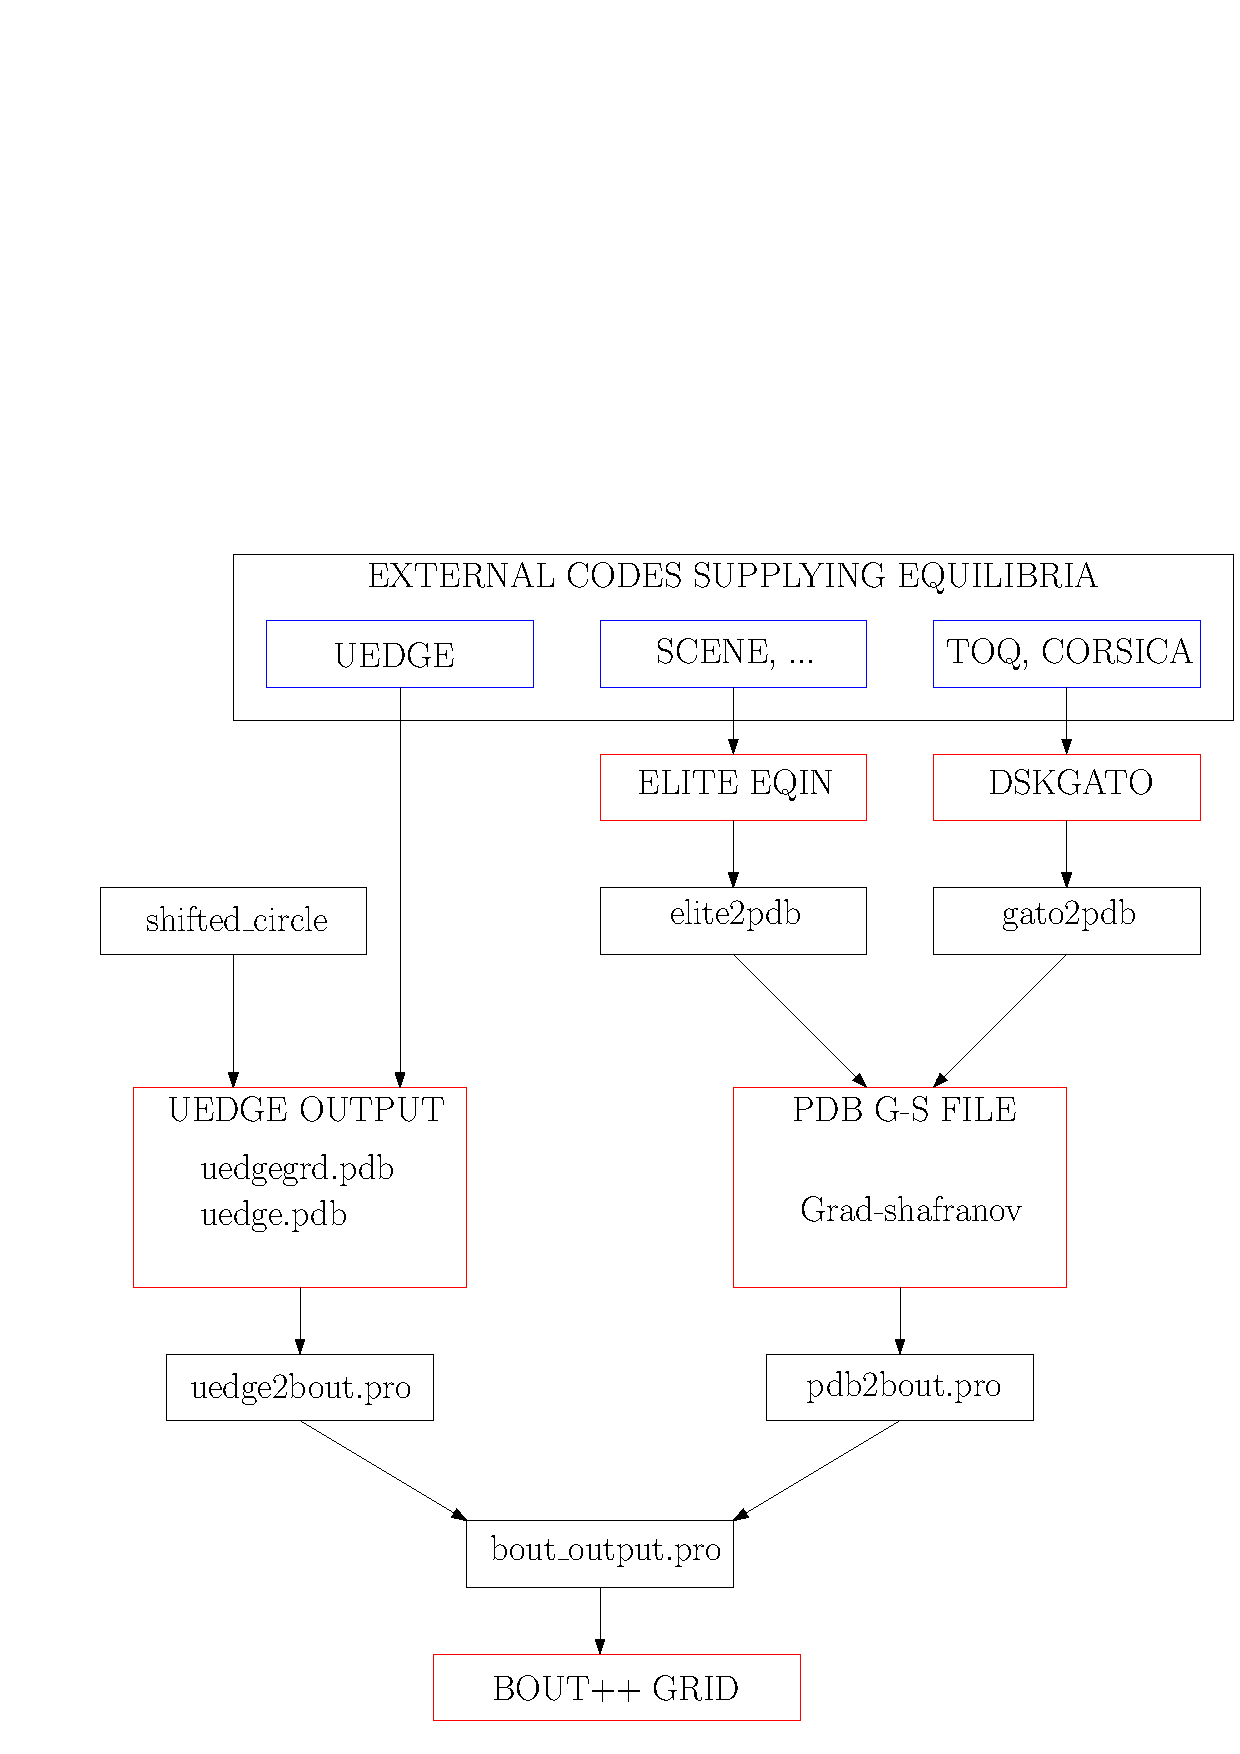
\includegraphics[width=0.7\paperwidth,
keepaspectratio]{figs/grid_gen.pdf}
\caption{Generation of BOUT++ grid files. In red are the file formats, and in 
black the conversion routines. Blue are external codes.}
%
\label{fig:gridgen}
%
\end{figure}
%
\clearpage



\subsection{BOUT++ Topology}
%


\subsubsection{Basic}
%
In order to handle tokamak geometry BOUT++ contains an internal topology which
is determined by the branch-cut locations (\code{jyseps1\_1},
\code{jyseps1\_2}, \code{jyseps2\_1}, and \code{jyseps2\_2}) and separatrix
locations (\code{ixseps1} and  \code{ixseps2}).

The separatrix locations, \code{ixseps1} and  \code{ixseps2}, give the indices
in the \code{x} domain where the first and second separatrices are located.

If \code{ixseps1 == ixseps2} then there is a single separatrix representing the
boundary between the core region and the SOL region and the grid is a connected
double null configuration. If \code{ixseps1 > ixseps2} then there are two
separatrices and the inner separatrix is \code{ixseps2} so the tokamak is an
upper double null. If \code{ixseps1 < ixseps2} then there are two separatrices
and the inner separatrix is \code{ixseps1} so the tokamak is a lower double
null.

In other words: Let us for illustrative purposes say that \code{ixseps1 >
ixseps2} (see figure \ref{fig:topology_cross_section}). Let us say that we have
a field \code{f(x,y,z)} with a global \code{x}-index which includes ghost
points. \code{f(x<=xseps1,y,z)}) will then be periodic in the
\code{y}-direction, \code{f(xspes1<x<=xseps2,y,z)}) will have boundary
condition in the \code{y}-direction set by the lowermost \code{ydown} and
\code{yup}.  If \code{f(xspes2<x,y,z)}) the boundary condition in the
\code{y}-direction will be set by the uppermost \code{ydown} and \code{yup}. As
for now, there is no difference between the two sets of upper and lower
\code{ydown} and \code{yup} boundary conditions (unless manually specified, see
section \ref{sec:custom_BC}).

These values are set either in the grid file or in \code{BOUT.inp}. Figure
\ref{fig:topology_cross_section} shows schematically how \code{ixseps} is used.

The branch cut locations, \code{jyseps1\_1}, \code{jyseps1\_2},
\code{jyseps2\_1}, and \code{jyseps2\_2}, split the \code{y} domain into
logical regions defining the SOL, the PFR (private flux region) and the core of
the tokamak. This is illustrated also in figure
\ref{fig:topology_cross_section}.  If \code{jyseps1\_2 == jyseps2\_1} then the
grid is a single null configuration, otherwise the grid is a double null
configuration.

%
\begin{figure}[htbp!]
\centering 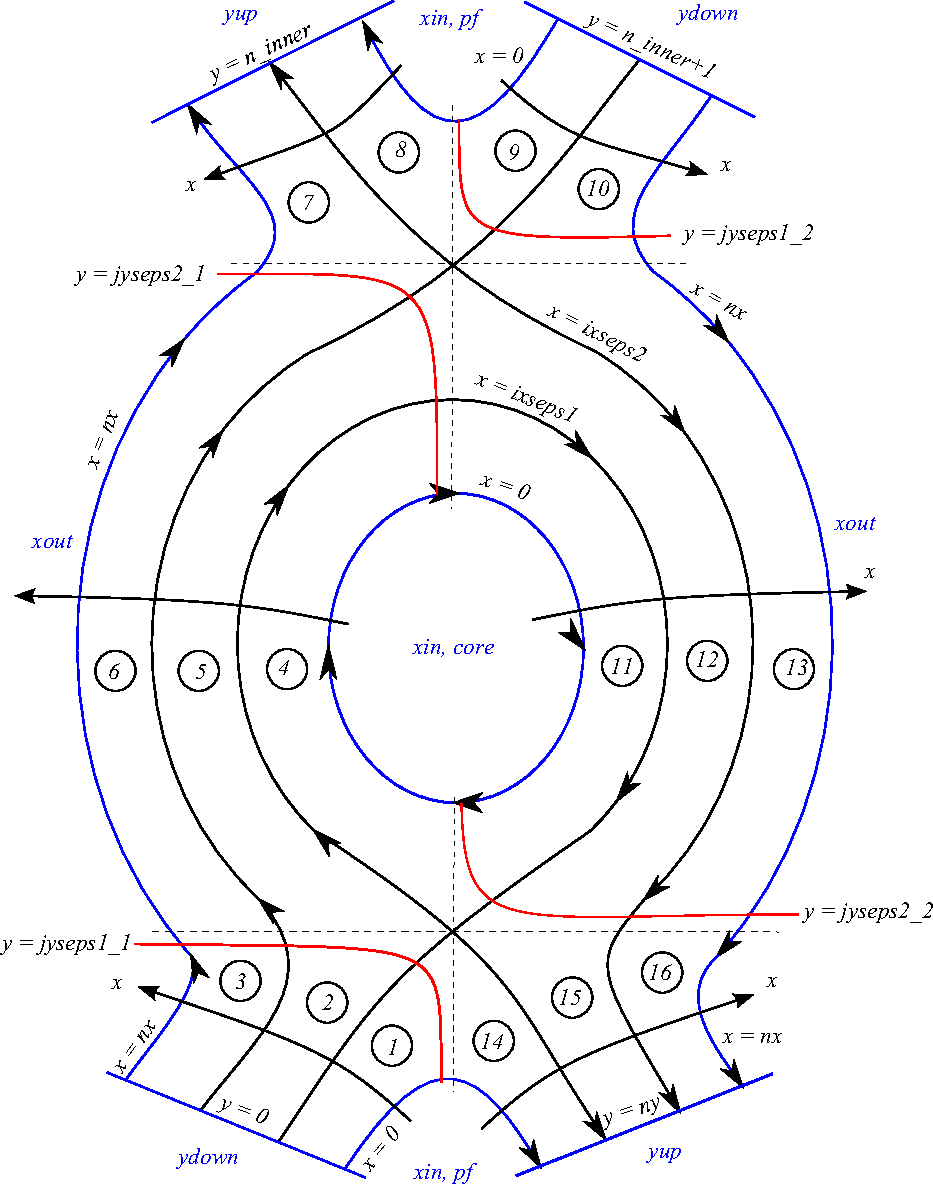
\includegraphics[width=0.7\paperwidth,
keepaspectratio]{figs/topology_cross_section.pdf}
\caption{Deconstruction of a poloidal tokamak cross-section into logical 
domains using the parameters \code{ixseps1}, \code{ixseps2}, \code{jyseps1\_1}, 
\code{jyseps1\_2}, \code{jyseps2\_1}, and \code{jyseps2\_2}.}
%
\label{fig:topology_cross_section}
%
\end{figure}
%


\subsubsection{Advanced}
%
The internal domain in BOUT++ is deconstructed into a series of logically
rectangular subdomains with boundaries determined by the \code{ixseps} and
\code{jyseps} parameters. The boundaries coinside with processor boundaries so
the number of grid points within each subdomain must be an integer multiple of
\code{ny/nypes} where \code{ny} is the number of grid points in \code{y} and
\code{nypes} is the number of processors used to split the y domain. Processor
communication across the domain boundaries is then handled internally. Figure
\ref{fig:topology_schematic} shows schematically how the different regions of a
double null tokamak with \code{ixseps1 = ixseps2} are connected together via
communications.

\note{To ensure that each subdomain follows logically, the \code{jyseps}
    indices must adhere to the following conditions:
%
\begin{itemize}
\item \code{jyseps1\_1 > -1}
\item \code{jyseps2\_1} $\geq$ \code{jyseps1\_1 + 1}
\item \code{jyseps1\_2} $\geq$ \code{jyseps2\_1}
\item \code{jyseps2\_2} $\leq$ \code{ny -1}
\end{itemize}
%
To ensure that communications work branch cuts must align with processor
boundaries.}

%
\begin{figure}[htbp!]
\centering 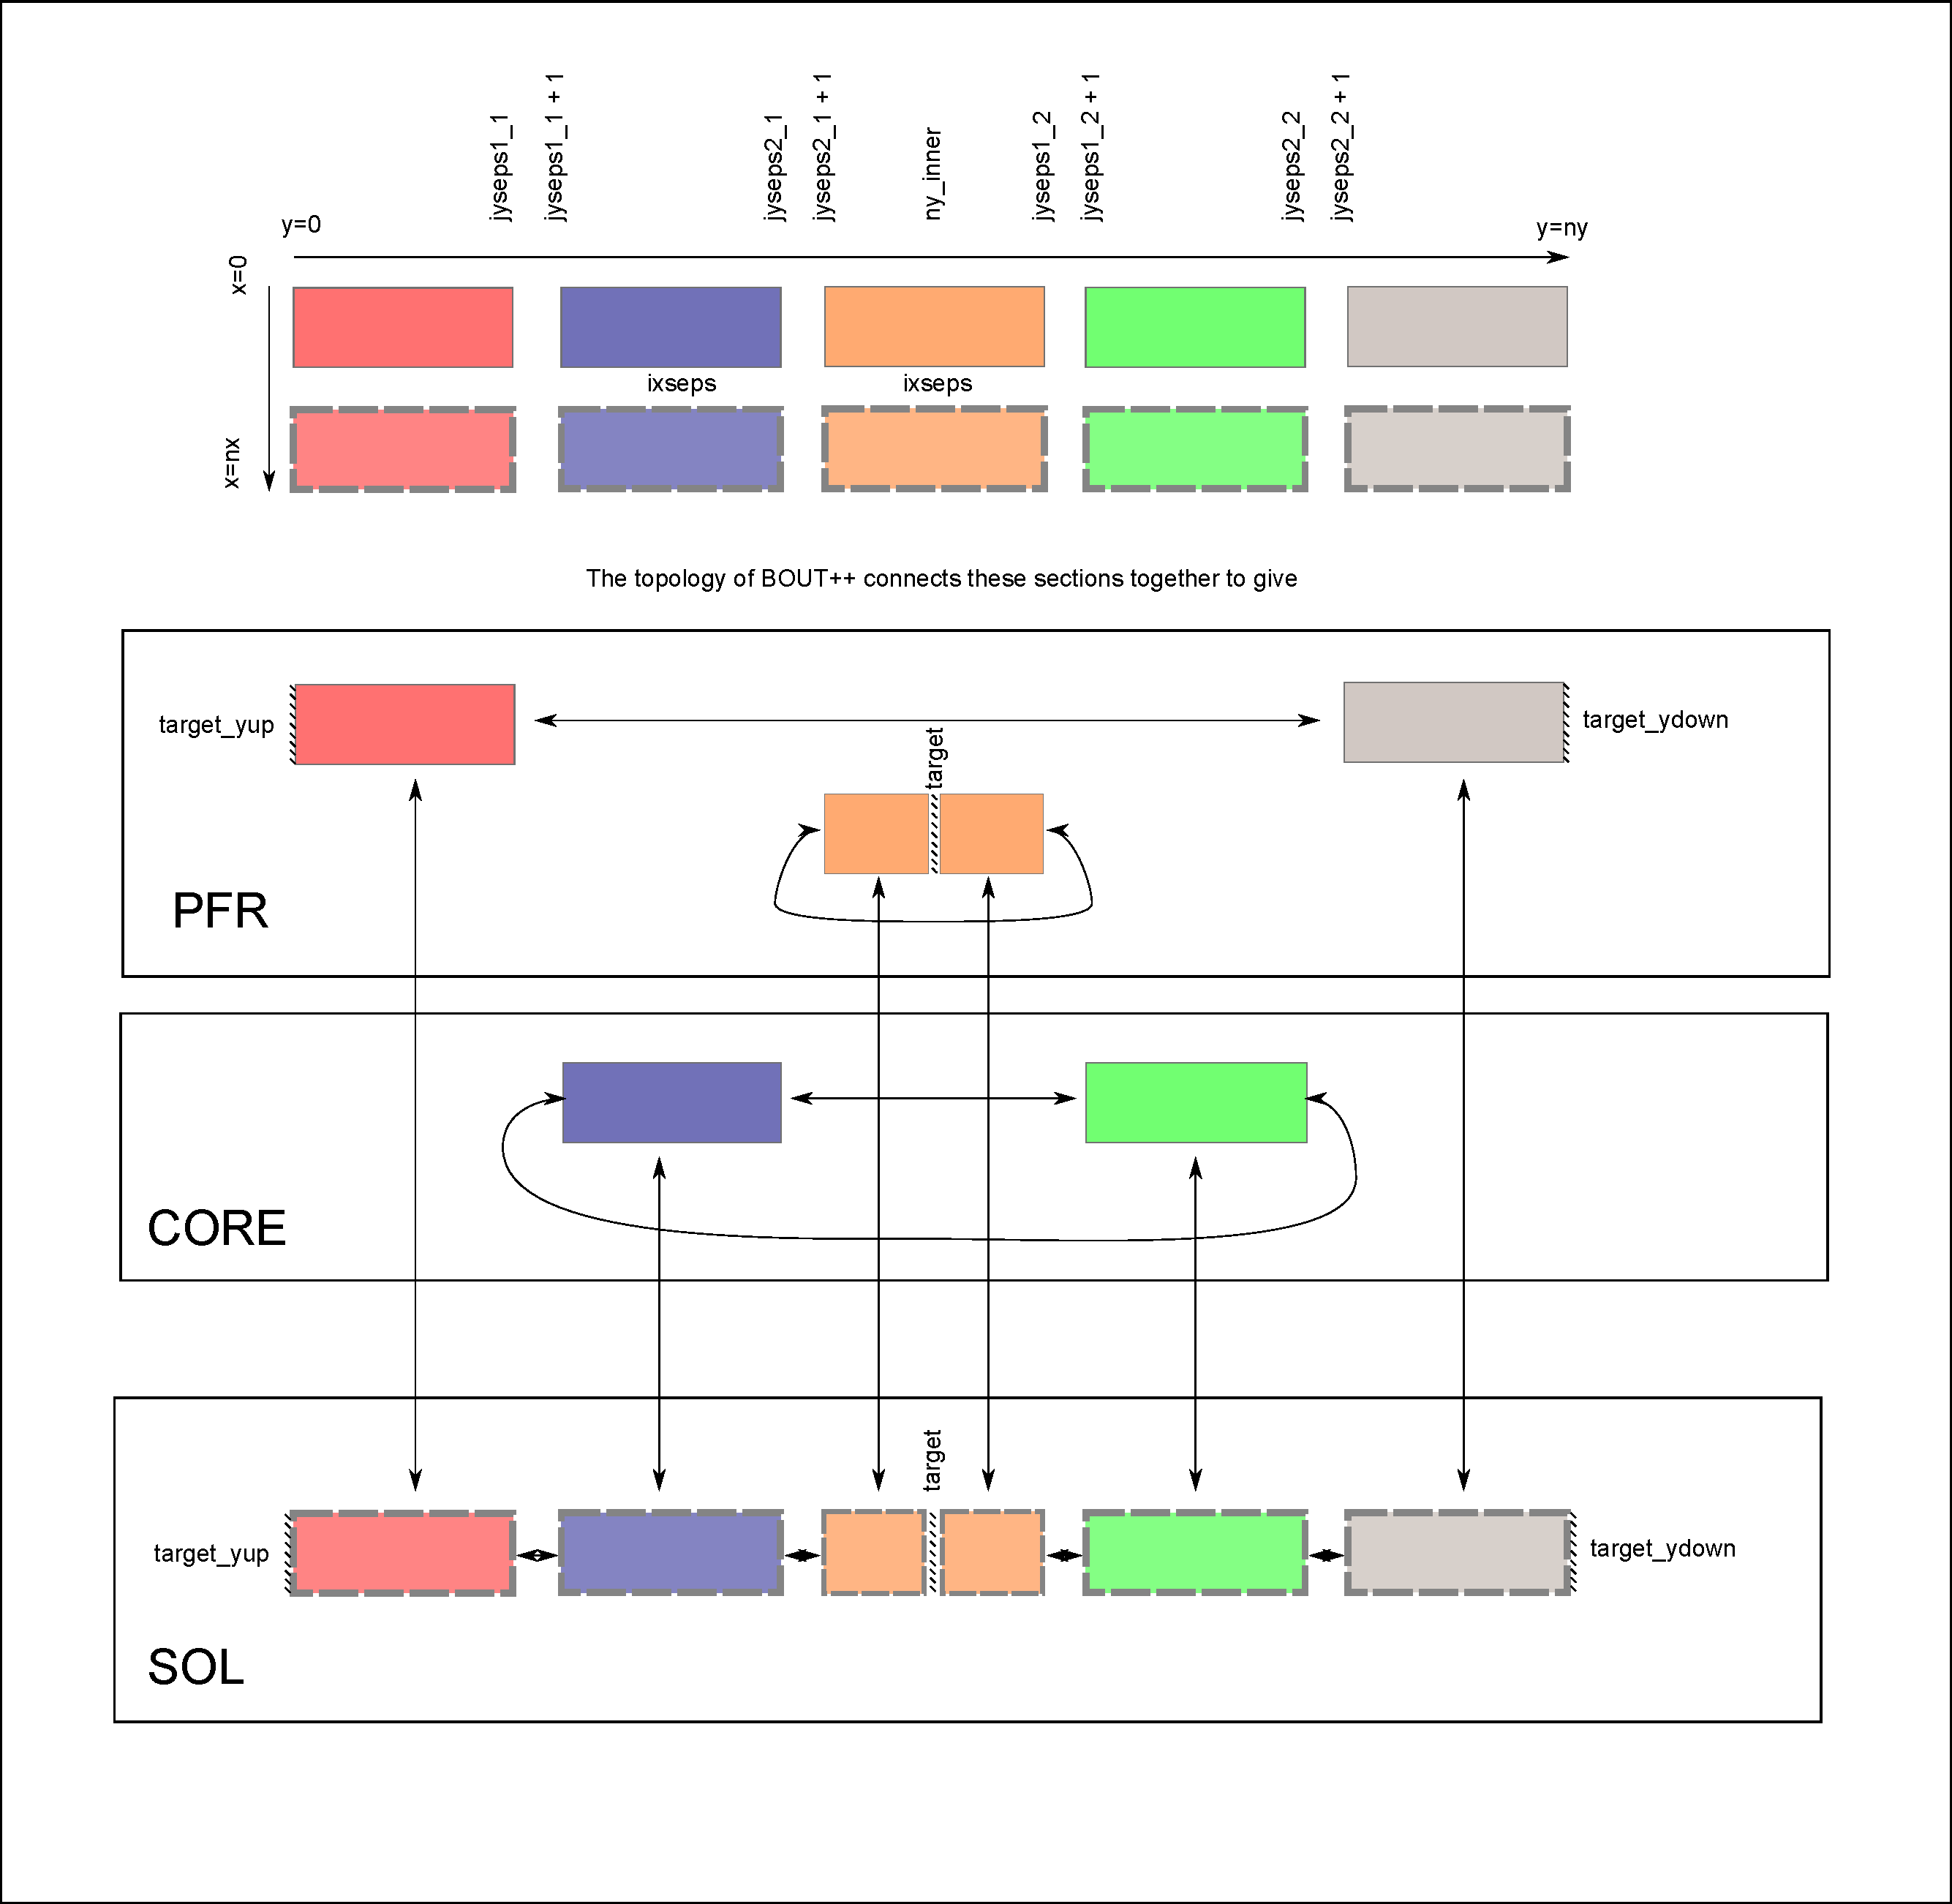
\includegraphics[width=\textwidth,
keepaspectratio]{figs/topology_schematic.pdf}
\caption{Schematic illustration of domain decomposition and communication in 
BOUT++ with \code{ixseps1 = ixseps2}.}
%
\label{fig:topology_schematic}
%
\end{figure}
%


\subsubsection{Implementations}
%



\subsection{3D variables}
%
BOUT++ was originally designed for tokamak simulations where the input
equilibrium varies only in X-Y, and Z is used as the axisymmetric toroidal
angle direction. In those cases, it is often convenient to have input grids
which are only 2D, and allow the Z dimension to be specified independently,
such as in the options file. The problem then is how to store 3D variables in
the grid file?

Two representations are now supported for 3D variables:
%
\begin{enumerate}
\item A Fourier representation. If the size of the toroidal domain is not
    specified in the grid file (\texttt{nz} is not defined), then 3D fields are
    stored as Fourier components. In the Z dimension the coefficients must be
    stored as
%
\begin{align}
\left[n = 0, n = 1 (\textrm{real}), n = 1 (\textrm{imag}), n = 2
(\textrm{real}), n = 2 (\textrm{imag}), \ldots \right]
\end{align}
%
where $n$ is the toroidal mode number. The size of the array must therefore be
odd in the Z dimension, to contain a constant ($n=0$) component followed by
real/imaginary pairs for the non-axisymmetric components.

If you are using IDL to create a grid file, there is a routine in
\texttt{tools/idllib/bout3dvar.pro} for converting between BOUT++'s real and
Fourier representation.

\item Real space, as values on grid points. If \texttt{nz} is set in the grid
    file, then 3D variables in the grid file must have size
    \texttt{nx}$\times$\texttt{ny}$\times$\texttt{nz}. These are then read in
    directly into \texttt{Field3D} variables as required.
\end{enumerate}
%



\subsection{From EFIT files}
%
\index{EFIT}\index{Hypnotoad}
%
An IDL code called ``Hypnotoad'' has been developed to create BOUT++ input
files from R-Z equilibria. This can read EFIT 'g' files, find flux surfaces,
and calculate metric coefficients.  The code is in
\file{tools/tokamak\_grids/gridgen}, and has its own manual under the
\file{doc} subdirectory.



\subsection{From ELITE and GATO files}
%
\index{ELITE}\index{GATO}\index{dskgato}
%
Currently conversions exist for ELITE \code{.eqin} and GATO \code{dskgato}
equilibrium files.  Conversion of these into BOUT++ input grids is in two
stages: In the first, both these input files are converted into a common NetCDF
or PDB format which describes the Grad-Shafranov equilibrium.  These
intermediate files are then converted to BOUT++ grids using an interactive IDL
script.



\subsection{Generating equilibria}
%
The directory \texttt{tokamak\_grids/shifted\_circle} contains IDL code to
generate shifted circle (large aspect ratio) Grad-Shafranov equilibria.



\subsection{Running pdb2bout}
%
There are many options which are set interactively, so here's a run-through of
the code (only showing most important outputs):

%
\begin{verbatim}
IDL> pdb2bout, "cbm18_dens6.dskgato.pdb", output="test.pdb"
***Maximum mu0p is       23071.7
Is this pressure (not mu0*pressure)?
\end{verbatim}
%
This is needed because although many grid formats claim to store $\mu_0 P$,
they actually store $P$. Since the given maximum value is very large, it must
be in Pascals, so answer yes (y).

The grid will then be displayed along with the safety factor and pressure
profiles against normalised $\psi$. In all three plots, a red line marks the
location of the plasma edge. You must then choose the radial domain in
normalised $\psi$:
%
\begin{verbatim}
Inner Psi boundary:0.6
Outer Psi boundary:1.2
Number of radial grid points:           69
Of which inside the plasma:           49
Is this range ok?
\end{verbatim}
%
The plots will now also show two green lines for the inner and outer
boundaries. Enter no (n) to specify a different range.

The code then checks to see if any plasma density of temperatures have been set
in the input file:
%
\begin{verbatim}
====== SETTING PLASMA PROFILES =======
Some plasma parameters given in input file
Use given parameters?
\end{verbatim}
%
Saying yes will just use the given values, but saying no will give you some
more options:
%
\begin{verbatim}
Generating plasma profiles:
  1. Flat temperature profile
  2. Flat density profile
  3. Te proportional to density
Profile option:
\end{verbatim}
%
The procedure is the same for each of these, so taking option 2 (flat density):
%
\begin{verbatim}
Setting flat density profile
Density [10^20 m^-3]:1.0
\end{verbatim}
%
Anything can be entered here, depending on what you want to simulate. The code
will ensure that whatever you enter, the equilibrium pressure is maintained. In
this case the temperature is calculated from pressure and the specified
density.
%
\begin{verbatim}
Maximum temperature (eV):      720.090
Is this ok?
\end{verbatim}
%
NOTE: This is the maximum temperature anywhere on the input grid (i.e. in this
case at $\psi = 0$), not just inside the chosen domain. Entering no will go
back and you can specify a different density.

Earlier the radial resolution was printed, in this case 69 grid points. You can
now change this if you need to:
%
\begin{verbatim}
Increase radial resolution?
\end{verbatim}
%
Although it says increase, you can also decrease the resolution. Entering yes
will allow you to enter a different number of radial grid points. It's
recommended to use $2^n + 4$ grid points because this makes it easier to
decompose the grid (4 cells for boundary, remainder equally divided between
processors).

At this point, an orthogonal grid is generated:
%
\begin{verbatim}
======== GENERATING ORTHOGONAL COORDINATES FOR BOUT =========
Number of poloidal grid points: 64
Enter x index of equal hthe [0, 68] :35
\end{verbatim}
%
Using  $2^n$ points is highly recommended, but only because the points must be
equally divided between processors.  The x index of equal hthe shouldn't matter
very much except for highly shaped plasmas. Recommend that you set it somewhere
around the peak pressure gradient, or middle of the grid.
%
\begin{verbatim}
Interpolating Rxy
Interpolating Zxy
Is this ok?
\end{verbatim}
%
Two plots are shown: On the left the original mesh, and on the right the new
orthogonal mesh. If this doesn't look right you can enter `no' and change the
poloidal resolution and location of equal $h_\theta$.

%
\begin{verbatim}
Add vacuum region?n
\end{verbatim}
%
This is a little experimental, and extends the grid into vacuum. This is useful
if the equilibrium supplied doesn't include a vacuum region. In this case we
already have a vacuum region, so can answer no.

You're now presented with several options:
%
\begin{verbatim}
Equilibrium correction options:
  0  No correction
  1  RBt using force balance
  2  hthe and RBt using force balance and q (FAILS)
  3  hthe and RBt using force balance and jpar
Enter option:
\end{verbatim}
%
Because the input Grad-Shafranov solution is probably not perfect to begin
with, and has now been interpolated onto a new grid, the force balance in
ballooning coordinates is not quite satisfied. These options attempt to correct
the equilibrium slightly to ensure force balance, the given $q$ profile, and
the given $j_{||}$ profile. Option 1 can sometimes work well, other times it
can fail to converge (as in this case). It's safe to just use option 0.

%
\begin{verbatim}
Calculating poloidal arc length dthe
Maximum difference in hthe:       0.23551123
Maximum percentage difference:        16.745859
Use new hthe?
\end{verbatim}
%
A key metric in the BOUT/BOUT++ coordinates is the poloidal arc length
$h_\theta$. A plot will shot this quantity calculated geometrically (solid
line), and calculated by enforcing force balance (red symbols) at the outboard
midplane.  The difference between these two methods is an indication of the
quality of the Grad-Shafranov solution. Entering 'y' will use the ``new''
$h_\theta$ calculated from force balance, whilst 'n' will use the $h_\theta$
calculated geometrically.  Personally. i prefer to make sure force balance is
satisfied so enter 'y'.

%
\begin{verbatim}
Checking parallel current
****Equilibrium has -ve toroidal field
\end{verbatim}
%
Because of the varied and confusing ways different codes define the poloidal
and toroidal directions, this code currently just sets Bp and Bt positive, and
then uses the expression for Jpar to work out what sign Bt should have.  This
is fine if you just want an equilibrium, but for detailed comparison to
experiment where the sign of Bt may/will make a difference this needs to be
changed.

Jpar calculated from quantities such as Bp, Bt and hthe is now shown as red
symbols, with the jpar from the original Grad-Shafranov solution as a black
line. Like the hthe display, this is a good consistency check.
%
\begin{verbatim}
Use new Jpar?
\end{verbatim}
%
Entering 'y' will use the calculated jpar i.e. consistent with the other grid
quantities, but probably more noisy and slightly different to the original.
Entering 'n' will use the original jpar profiles.

%
\begin{verbatim}
q is negative. Reversing values from equilibrium
\end{verbatim}
%
This can be printed because the $q$ profile given in the grid file is almost
always positive, whereas qsafe calculated by integrating the pitch angle can be
positive or negative. In this case the toroidal field has been set negative
(see above), and so qinty is negative too.

%
\begin{verbatim}
Use new qsafe?
\end{verbatim}
%
As with hthe and jpar, the qsafe specified in the original grid file is plotted
as a black line, and the value calculated by integrating quantities on the new
mesh is shown as red symbols. Entering 'y' uses the values consistent on the
new grid, whilst 'n' uses the original safety factor profile. In most cases i'd
prefer the grid to be consistent, rather than being identical to the input, so
answer 'y'. You may have to do some experimentation though.

%
\begin{verbatim}
****Minimum pressure is very small:       0.0000000
****Setting minimum pressure to 1% of maximum
\end{verbatim}
%
This is because having negative pressures is very bad for BOUT/BOUT++ runs, and
can easily be caused by overshoots or even rounding error when the pressure is
too low. Because the equilibrium doesn't depend on absolute pressure, this just
adds a constant pressure across the entire profile.

Finally, the grid file is written to PDB format
%
\begin{verbatim}
Cannot write 2 dimensional double dx. Writing as float
.
.
.
\end{verbatim}
%
These warnings are because the PDB2IDL library currently doesn't have any
functions for writing doubles, and pdb2bout does calculations in double
precision. The output is therefore converted to single-precision floats.





\section{Fluid equations}
%
\label{sec:equations}
%
Once you have tried some example codes, and generally got the hang of running
BOUT++ and analysing the results, there will probably come a time when you want
to change the equations being solved.  This section uses the ideal MHD
equations as an example, demonstrating how a BOUT++ physics module is put
together. It assumes you have a working knowledge of C or C++, but you don't
need to be an expert - most of the messy code is hidden away from the physics
module. There are several good books on C and C++, but I'd recommend online
tutorials over books because there are a lot more of them, they're quicker to
scan through, and they're cheaper.

When going through this section, it may help to refer to the finished code,
which is given in the file \texttt{mhd.cxx} in the BOUT++ examples directory.
The equations to be solved are:
%
\begin{align*}
\deriv{\rho}{t} =& -\mathbf{v}\cdot\nabla\rho - \rho\nabla\cdot\mathbf{v} \\
    \deriv{p}{t} =& -\mathbf{v}\cdot\nabla p - \gamma p\nabla\cdot\mathbf{v} \\
    \deriv{\mathbf{v}}{t} =& -\mathbf{v}\cdot\nabla\mathbf{v} +
    \frac{1}{\rho}\left(-\nabla p +
    \left(\nabla\times\mathbf{B}\right)\times\mathbf{B}\right) \\
    \deriv{\mathbf{B}}{t} =&
    \nabla\times\left(\mathbf{v}\times\mathbf{B}\right)
\end{align*}
%
There are two ways to specify a set of equations to solve in BOUT++. For
advanced users, an object-oriented interface is available and described in
section~\ref{sec:newapi}. The simplest way to start is to use a C-like
interface and define two functions:
%
\begin{lstlisting}
int physics_init(bool restarting) {
  return 0;
}

int physics_run(BoutReal t) {
  return 0;
}
\end{lstlisting}
%
The first of these is called once at the start of the simulation, and should
set up the problem, specifying which variables are to be evolved. The argument
\code{restarting} is false the first time a problem is run, and true if loading
the state from a restart file.

The second function \code{physics\_run} is called every time-step, and should
calculate the time-derivatives for a given state. In both cases returning
non-zero tells BOUT++ that an error occurred.



\subsection{Variables}
%
We need to define the variables to evolve as global variables (so they can be
used in \code{physics\_init} and \code{physics\_run}.

\note{Version 0.85 and earlier needed two variables to be defined, so if you're
upgrading then you can remove the time-derivative variables}

For ideal MHD, we need two 3D scalar fields density $\rho$ and pressure $p$,
and two 3D vector fields velocity $v$, and magnetic field $B$:
%
\begin{lstlisting}
Field3D rho, p; // 3D scalar fields
Vector3D v, B;  // 3D vector fields

int physics_init(bool restarting) {
}
\end{lstlisting}
%
Scalar and vector fields behave much as you would expect:
%
\lstinline!Field3D!
%
 objects can be added, subtracted, multiplied, divided and exponentiated, so
 the following examples are all valid operations:
%
\index{Field3D}\index{BoutReal}
%
\begin{lstlisting}
Field3D a, b, c;
BoutReal r;

a = b + c; a = b - c;
a = b * c; a = r * b;
a = b / c; a = b / r; a = r / b;
a = b ^ c; a = b ^ r; a = r ^ b;
\end{lstlisting}
%
Similarly, vector objects can be added/subtracted from each other,
multiplied/divided by scalar fields and real numbers, for example:
%
\index{Vector3D}
%
\begin{lstlisting}
Vector3D a, b, c;
Field3D f;
BoutReal r;

a = b + c; a = b - c;
a = b * f; a = b * r;
a = b / f; a = b / r;
\end{lstlisting}
%
In addition the dot and cross products are represented by \code{*} and \pow
symbols:
%
\begin{lstlisting}
Vector3D a, b, c;
Field3D f;

f = a * b // Dot-product
a = b ^ c // Cross-product
\end{lstlisting}
%
For both scalar and vector field operations, so long as the result of an
operation is of the correct type, the usual C/C++ shorthand notation can be
used:
%
\begin{lstlisting}
Field3D a, b;
Vector3D v, w;

a += b; v *= a; v -= w; v ^= w; // valid
v *= w; // NOT valid: result of dot-product is a scalar
\end{lstlisting}
%
\parbox{\textwidth}

\note{In C++ the \pow operator has lower precedence than the \code{*} or
\code{+} operators.  To be safe, always put exponentiation and cross-product
operations in brackets}



\subsection{Evolution equations}
%
At this point we can tell BOUT++ which variables to evolve, and where the state
and time-derivatives will be stored. This is done using the
\code{bout\_solve(variable, name)} function in \code{physics\_init}:
%
\begin{lstlisting}
int physics_init(bool restarting) {
  bout_solve(rho, "density");
  bout_solve(p,   "pressure");
  bout_solve(v,   "v");
  bout_solve(B,   "B");

  return 0;
}
\end{lstlisting}
%
The name given to this function will be used in the output and restart data
files. These will be automatically read and written depending on input options
(see section~\ref{sec:options}).  Input options based on these names are also
used to initialise the variables.

If the name of the variable in the output file is the same as the variable
name, you can use a shorthand macro. In this case, we could use this shorthand
for \code{v} and \code{B}:
%
\index{SOLVE\_FOR}
%
\begin{lstlisting}
SOLVE_FOR(v);
SOLVE_FOR(B);
\end{lstlisting}
%
To make this even shorter, we can use macros \code{SOLVE\_FOR2},
\code{SOLVE\_FOR3}, ..., \code{SOLVE\_FOR6} to shorten our initialisation code
to
%
\begin{lstlisting}
int physics_init(bool restarting) {
  bout_solve(rho, "density");
  bout_solve(p,   "pressure");
  SOLVE_FOR2(v, B);

  return 0;
}
\end{lstlisting}
%
The equations to be solved can now be written in the \code{physics\_run}
function. The value passed to the function (\code{BoutReal t}) is the
simulation time - only needed if your equations contain time-dependent sources
or similar terms. To refer to the time-derivative of a variable \code{var}, use
\code{ddt(var)}. The ideal MHD equations can be written as:
%
\begin{lstlisting}
int physics_run(BoutReal t) {
  ddt(rho) = -V_dot_Grad(v, rho) - rho*Div(v);
  ddt(p) = -V_dot_Grad(v, p) - gamma*p*Div(v);
  ddt(v) = -V_dot_Grad(v, v) + ( (Curl(B)^B) - Grad(p) ) / rho;
  ddt(B) = Curl(v^B);
}
\end{lstlisting}
%
Where the differential operators \code{vector = Grad(scalar)}, \code{scalar =
Div(vector)}, and \code{vector = Curl(vector)} are used. For the density and
pressure equations, the $\mathbf{v}\cdot\nabla\rho$ term could be written as
\code{v*Grad(rho)}, but this would then use central differencing in the Grad
operator. Instead, the function \code{V\_dot\_Grad} uses upwinding methods for
these advection terms. In addition, the \code{Grad} function will not operate
on vector objects (since result is neither scalar nor vector), so the
$\mathbf{v}\cdot\nabla\mathbf{v}$ term CANNOT be written as \code{v*Grad(v)}.



\subsection{Input options}
%
\label{sec:inputopts}
%
\index{Options}
%
Note that in the above equations the extra parameter \code{gamma} has been
used. To enable this to be set in the input options file (see
section~\ref{sec:options}), we use the \code{options} object in the
initialisation function:
%
\begin{lstlisting}
BoutReal gamma;

int physics_init(bool restarting) {
  Options *globalOptions = Options::getRoot();
  Options *options = globalOptions->getSection("mhd");

  options->get("gamma", gamma, 5.0/3.0);
\end{lstlisting}
%
This specifies that an option called ``gamma'' in a section called ``mhd''
should be put into the variable \code{gamma}. If the option could not be found,
or was of the wrong type, the variable should be set to a default value of
$5/3$.  The value used will be printed to the output file, so if gamma is not
set in the input file the following line will appear:
%
\begin{verbatim}
      Option mhd / gamma = 1.66667 (default)
\end{verbatim}
%
This function can be used to get integers and booleans. To get strings, there
is the function (\code{char* options.getString(section, name)}.  To separate
options specific to the physics model, these options should be put in a
separate section, for example here the ``mhd'' section has been specified. To
save having to write the section name for every option, there is the
\code{setSection} function:
%
\begin{lstlisting}
BoutReal gamma;
int someint;

int physics_init(bool restarting) {
  Options *globalOptions = Options::getRoot();
  Options *options = globalOptions->getSection("mhd");

  options->get("gamma", gamma, 5.0/3.0);
  options->get("someint", someint, 0);
\end{lstlisting}
%
Most of the time, the name of the variable (e.g. \code{gamma}) will be the same
as the identifier in the options file (``gamma''). In this case, there is the
macro
%
\begin{lstlisting}[numbers=none]
OPTION(options, gamma, 5.0/3.0);
\end{lstlisting}
%
which is equivalent to
%
\begin{lstlisting}[numbers=none]
options->get("gamma", gamma, 5.0/3.0);
\end{lstlisting}
%
See section~\ref{sec:options} for more details of how to use the input options.



\subsection{Communication}
%
\index{communication}
%
If you plan to run BOUT++ on more than one processor, any operations involving
y derivatives will require knowledge of data stored on other processors. To
handle the necessary parallel communication, there is the
\code{mesh->communicate} function. This takes care of where the data needs to
go to/from, and only needs to be told which variables to transfer.

If you only need to communicate a small number (up to 5 currently) of variables
then just call the \code{mesh->communicate} function directly. For the MHD
code, we need to communicate the variables \code{rho,p,v,B} at the beginning of
the \code{physics\_run} function before any derivatives are calculated:
%
\begin{lstlisting}
int physics_run(BoutReal t) {
  mesh->communicate(rho, p, v, B);
\end{lstlisting}
%
If you need to communicate lots of variables, or want to change at run-time
which variables are evolved (e.g. depending on input options), then you can
create a group of variables and communicate them later.  To do this, first
create a \code{FieldGroup} object
%
\index{FieldGroup}, in this case called \code{comms}
%
, then use the add method. This method does no communication, but records which
variables to transfer when the communication is done later.
%
\begin{lstlisting}
FieldGroup comms;

int physics_init() {
  .
  .
  .
  comms.add(rho);
  comms.add(p);
  comms.add(v);
  comms.add(B);

  return 0;
}
\end{lstlisting}
%
The
%
\lstinline!comms.add()!
%
 routine can be given up to 6 variables at once (there's no practical limit on
 the total number of variables which are added to a
%
\lstinline!FieldGroup!
%
), so this can be shortened to
%
\begin{lstlisting}
FieldGroup comms;

int physics_init() {
  .
  .
  .
  comms.add(rho, p, v, B);

  return 0;
}
\end{lstlisting}
%
To perform the actual communication, call the \code{mesh->communicate} function
with the group. In this case we need to communicate all these variables before
performing any calculations, so call this function at the start of the
\code{physics\_run} routine:
%
\begin{lstlisting}
int physics_run(BoutReal t) {
  mesh->communicate(comms);
  .
  .
  .
\end{lstlisting}
%
In many situations there may be several groups of variables which can be
communicated at different times. The function \code{mesh->communicate} consists
of a call to \code{mesh->send} followed by \code{mesh->wait} which can be done
separately to interleave calculations and communications. This will speed up
the code if parallel communication bandwidth is a problem for your simulation.

In our MHD example, the calculation of \code{ddt(rho)} and \code{ddt(p)} does
not require \code{B}, so we could first communicate \code{rho}, \code{p}, and
\code{v}, send \code{B} and do some calculations whilst communications are
performed:
%
\index{comm\_handle}
%
\begin{lstlisting}
int physics_run(BoutReal t) {
  mesh->communicate(rho, p, v); // sends and receives rho, p and v
  comm_handle ch = mesh->send(B);// only send B

  ddt(rho) = ...
  ddt(p) = ...

  mesh->wait(ch); // now wait for B to arrive

  ddt(v) = ...
  ddt(B) = ...

  return 0;
}
\end{lstlisting}
%
This scheme is not used in \texttt{mhd.cxx}, partly for clarity, and partly
because currently communications are not a significant bottleneck (too much
inefficiency elsewhere!).

\note{Before using the result of a differential operator as input to another
differential operator, communications must be performed for the intermediate
result}

When a differential is calculated, points on neighbouring cells are assumed to
be in the guard cells.  There is no way to calculate the result of the
differential in the guard cells, and so after every differential operator the
values in the guard cells are invalid. Therefore, if you take the output of one
differential operator and use it as input to another differential operator, you
must perform communications (and set boundary conditions) first. See
section~\ref{sec:diffops}.



\subsection{Boundary conditions}
%
\index{boundary conditions}
%
All evolving variables have boundary conditions applied automatically after the
%
\lstinline!physics_run!
%
 has finished. Which condition is applied depends on the options file settings
 (see section~\ref{sec:bndryopts}). If you want to disable this and apply your
 own boundary conditions then set boundary condition to \code{none} in the
 \code{BOUT.inp} options file.

In addition to evolving variables, it's sometimes necessary to impose boundary
conditions on other quantities which are not explicitly evolved.

The simplest way to set a boundary condition is to specify it as text, so to
apply a Dirichlet boundary condition:
%
\begin{lstlisting}
  Field3D var;
  ...
  var.applyBoundary("dirichlet");
\end{lstlisting}
%
The format is exactly the same as in the options file. Each time this is called
it must parse the text, create and destroy boundary objects. To avoid this
overhead and have different boundary conditions for each region, it's better to
set the boundary conditions you want to use first in \code{physics\_init}, then
just apply them every time:
%
\begin{lstlisting}
Field3D var;

int physics_init() {
  ...
  var.setBoundary("myVar");
  ...
}

int physics_run(BoutReal t) {
  ...
  var.applyBoundary();
  ...
}
\end{lstlisting}
%
This will look in the options file for a section called \code{"[myvar]"} (upper
or lower case doesn't matter) in the same way that evolving variables are
handled. In fact this is precisely what is done: inside \code{bout\_solve} (or
\code{SOLVE\_FOR}) the \code{setBoundary} method is called, and then after
\code{physics\_run} the applyBoundary() method is called on each evolving
variable.  This method also gives you the flexibility to apply different
boundary conditions on different boundary regions (e.g. radial boundaries and
target plates); the first method just applies the same boundary condition to
all boundaries.

Another way to set the boundaries is to copy them from another variable:
%
\begin{lstlisting}
Field3D a, b;
  ...
  a.setBoundaryTo(b); // Copy b's boundaries into a
  ...
\end{lstlisting}
%


\subsubsection{Custom boundary conditions}
%
\label{sec:custom_BC}
%
The boundary conditions supplied with the BOUT++ library cover the most common
situations, but cannot cover all of them. If the boundary condition you need
isn't available, then it's quite straightforward to write your own. First you
need to make sure that your boundary condition isn't going to be overwritten.
To do this, set the boundary condition to ``none'' in the BOUT.inp options
file, and BOUT++ will leave that boundary alone. For example:
%
\begin{lstlisting}
[P]
bndry_all = dirichlet
bndry_xin = none
bndry_xout = none
\end{lstlisting}
%
would set all boundaries for the variable ``P'' to zero value, except for the X
inner and outer boundaries which will be left alone for you to modify.

To set an X boundary condition, it's necessary to test if the processor is at
the left boundary (first in X), or right boundary (last in X). Note that it
might be both if \code{NXPE = 1}, or neither if \code{NXPE > 2}.
%
\begin{lstlisting}
  Field3D f;
  ...
  if(mesh->firstX()) {
    // At the left of the X domain
    // set f[0:1][*][*] i.e. first two points in X, all Y and all Z
    for(int x=0; x < 2; x++)
      for(int y=0; y < mesh->ngy; y++)
        for(int z=0; z < mesh->ngz; z++) {
          f[x][y][z] = ...
        }
  }
  if(mesh->lastX()) {
    // At the right of the X domain
    // Set last two points in X
    for(int x=mesh->ngx-2; x < mesh->ngx; x++)
      for(int y=0; y < mesh->ngy; y++)
        for(int z=0; z < mesh->ngz; z++) {
          f[x][y][z] = ...
        }
  }
\end{lstlisting}
%
note the size of the local mesh including guard cells is given by
\code{mesh->ngx}, \code{mesh->ngy}, and \code{mesh->ngz}. The functions
\code{mesh->firstX()} and \code{mesh->lastX()} return true only if the current
processor is on the left or right of the X domain respectively.

Setting custom Y boundaries is slightly more complicated than X boundaries,
because target or limiter plates could cover only part of the domain. Rather
than use a \code{for} loop to iterate over the points in the boundary, we need
to use a more general iterator:

%
\begin{lstlisting}
  Field3D f;
  ...
  RangeIterator it = mesh->iterateBndryLowerY();
  for(it.first(); !it.isDone(); it++) {
    // it.ind contains the x index
    for(int y=2;y>=0;y--)  // Boundary width 3 points
      for(int z=0;z<mesh->ngz;z++) {
        ddt(f)[it.ind][y][z] = 0.;  // Set time-derivative to zero in boundary
      }
  }
\end{lstlisting}
%
This would set the time-derivative of f to zero in a boundary of width 3 in Y
(from 0 to 2 inclusive). In the same way
%
\lstinline!mesh->iterateBndryUpperY()!
%
 can be used to iterate over the upper boundary:
%
\begin{lstlisting}
  RangeIterator it = mesh->iterateBndryUpperY();
  for(it.first(); !it.isDone(); it++) {
    // it.ind contains the x index
    for(int y=mesh->ngy-3;y<mesh->ngy;y--)  // Boundary width 3 points
      for(int z=0;z<mesh->ngz;z++) {
        ddt(f)[it.ind][y][z] = 0.;  // Set time-derivative to zero in boundary
      }
  }
\end{lstlisting}
%



\subsection{Initial profiles}
%
\index{variable initialisation}
%
Up to this point the code is evolving total density, pressure etc. This has
advantages for clarity, but has problems numerically: For small perturbations,
rounding error and tolerances in the time-integration mean that linear
dispersion relations are not calculated correctly. The solution to this is to
write all equations in terms of an initial ``background'' quantity and a
time-evolving perturbation, for example $\rho\left(t\right) \rightarrow \rho_0
+ \tilde{\rho}\left(t\right)$.  For this reason, {\bf the initialisation of all
variables passed to the \code{bout\_solve} function is a combination of
small-amplitude gaussians and waves; the user is expected to have performed
this separation into background and perturbed quantities.}

To read in a quantity from a grid file, there is the \code{grid.get} function:

%
\begin{lstlisting}
Field2D Ni0; // Background density

int physics_init(bool restarting) {
  ...
  mesh->get(Ni0, "Ni0");
  ...
}
\end{lstlisting}
%
As with the input options, most of the time the name of the variable in the
physics code will be the same as the name in the grid file to avoid confusion.
In this case, you can just use
%
\index{GRID\_LOAD}
%
\begin{lstlisting}
GRID_LOAD(Ni0);
\end{lstlisting}
%
which is equivalent to
%
\begin{lstlisting}
mesh->get(Ni0, "Ni0");
\end{lstlisting}
%



\subsection{Output variables}
%
BOUT++ always writes the evolving variables to file, but often it's useful to
add other variables to the output. For convenience you might want to write the
normalised starting profiles or other non-evolving values to file. For example:
%
\begin{lstlisting}
  Field2D Ni0;
  ...
  GRID_LOAD(Ni0);
  dump.add(Ni0, "Ni0", 0);
\end{lstlisting}
%
where the '0' at the end means the variable should only be written to file once
at the start of the simulation. For convenience there are some macros e.g.
%
\index{SAVE\_ONCE}
%
\begin{lstlisting}
  SAVE_ONCE(Ni0);
\end{lstlisting}
%
is equivalent to
%
\begin{lstlisting}
  dump.add(Ni0, "Ni0", 0);
\end{lstlisting}
%
In some situations you might also want to write some data to a different file.
To do this, create a Datafile object:

%
\begin{lstlisting}
Datafile mydata;
\end{lstlisting}
%
in physics\_init, you then:

%
\begin{enumerate}
\item (optional) Initialise the file, passing it the options to use. If you
    skip this step, default (sane) options will be used. This just allows you
    to enable/disable, use parallel I/O, set whether files are opened and
    closed every time etc.
%
\begin{lstlisting}
mydata = Datafile(Options::getRoot()->getSection("mydata"));
\end{lstlisting}
%
which would use options in a section [mydata] in BOUT.inp

\item Open the file for writing
%
\begin{lstlisting}
mydata.openw("mydata.nc")
\end{lstlisting}
%
By default this only specifies the file name; actual opening of the file
happens later when the data is written. If you are not using parallel I/O, the
processor number is also inserted into the file name before the last ``.'', so
mydata.nc'' becomes ``mydata.0.nc'', ``mydata.1.nc'' etc. The file format used
depends on the extension, so ``.nc'' will open NetCDF, ``.hdf5'' an HDF5 file,
``.pdb'' a PDB file etc.

(see e.g. src/fileio/datafile.cxx line 139, which calls
src/fileio/dataformat.cxx line 23, which then calls the file format interface
e.g. src/fileio/impls/netcdf/nc\_format.cxx line 172).

\item Add variables to the file
%
\begin{lstlisting}
mydata.add(variable, "name") ;  // Not evolving. Every time the file is 
written, this will be overwritten
mydata.add(variable2, "name2", 1); // Evolving. Will output a sequence of values
\end{lstlisting}
%
\end{enumerate}
%
Whenever you want to write values to the file, for example in physics\_run or a
monitor, just call
%
\begin{lstlisting}
mydata.write();
\end{lstlisting}
%
To collect the data afterwards, you can specify the prefix to collect. In
Python:
%
\begin{verbatim}
>>> var = collect("name", prefix="mydata")
\end{verbatim}
%
or in IDL:
%
\begin{verbatim}
IDL> var = collect(var="name", prefix="mydata")
\end{verbatim}
%
By default the prefix is "BOUT.dmp".





\section{Fluid equations 2: reduced MHD}
%
The MHD example presented previously covered some of the functions available in
BOUT++, which can be used for a wide variety of models. There are however
several other significant functions and classes which are commonly used, which
will be illustrated using the \texttt{reconnect-2field} example. This is
solving equations for $A_{||}$ and vorticity $U$

%
\begin{align*}
\deriv{U}{t} =& -\frac{1}{B}\mathbf{b}_0\times\nabla\phi\cdot\nabla U + B^2
    \nabla_{||}\left(j_{||} / B\right) \\ \deriv{A_{||}}{t} =&
    -\frac{1}{\hat{\beta}}\nabla_{||}\phi - \eta\frac{1}{\hat{\beta}} j_{||}
\end{align*}
%
with $\phi$ and $j_{||}$ given by
%
\begin{align*}
U =& \frac{1}{B}\nabla_\perp^2\phi \\ j_{||} =& -\nabla_\perp^2 A_{||}
\end{align*}
%
First create the variables which are going to be evolved, ensure they're
communicated

%
\begin{lstlisting}
Field3D U, Apar; // Evolving variables

int physics_init(bool restarting) {

  SOLVE_FOR2(U, Apar);
}

int physics_run(BoutReal t) {
  mesh->communicate(U, Apar);

}
\end{lstlisting}
%
In order to calculate the time derivatives, we need the auxiliary variables
$\phi$ and $j_{||}$. Calculating $j_{||}$ from $A_{||}$ is a straightforward
differential operation, but getting $\phi$ from $U$ means inverting a
Laplacian.
%
\begin{lstlisting}
Field3D U, Apar;
Field3D phi, jpar; // Auxilliary variables

int physics_init(bool restarting) {
  SOLVE_FOR2(U, Apar);
  SAVE_REPEAT2(phi, jpar); // Save variables in output file
  return 0;
}

int physics_run(BoutReal t) {
  phi = invert_laplace(mesh->Bxy*U, phi_flags); // Solve for phi
  mesh->communicate(U, Apar, phi);  // Communicate phi
  jpar = -Delp2(Apar);     // Calculate jpar
  mesh->communicate(jpar); // Communicate jpar
  return 0;
}
\end{lstlisting}
%
Note that the Laplacian inversion code takes care of boundary regions, so
%
\lstinline!U!
%
 doesn't need to be communicated first. The differential operator
%
\lstinline!Delp2!
%
, like all differential operators, needs the values in the guard cells and so
%
\lstinline!Apar!
%
 needs to be communicated before calculating
%
\lstinline!jpar!
%
. Since we will need to take derivatives of
%
\lstinline!jpar!
%
 later, this needs to be communicated as well.
%
\begin{lstlisting}
int physics_run(BoutReal t) {
  ...
  mesh->communicate(jpar);

  ddt(U) = -b0xGrad_dot_Grad(phi, U) + SQ(mesh->Bxy)*Grad_par(Jpar / mesh->Bxy)
  ddt(Apar) = -Grad_par(phi) / beta_hat - eta*jpar / beta_hat; }
\end{lstlisting}
%



\subsection{Printing messages/warnings}
%
\label{sec:printing}
%
In order to print to screen and/or a log file, the object \code{output} is
provided.  This provides two different ways to write output: the C
(\code{printf}) way, and the C++ stream way. This is because each method can be
clearer in different circumstances, and people have different tastes in these
matters.

The C-like way (which is the dominant way in BOUT++) is to use the \code{write}
function, which works just like \code{printf}, and takes all the same codes (it
uses \code{sprintf} internally).
%
\index{output}
%
\begin{lstlisting}
output.write(const char *format, ...)
\end{lstlisting}
%
For example:
%
\begin{lstlisting}
output.write("This is an integer: %d, and this a real: %e\n", 5, 2.0)
\end{lstlisting}
%
For those who prefer the C++ way of doing things, a completely equivalent way
is to treat \code{output} as you would \code{cout}:
%
\begin{lstlisting}
output << "This is an integer: " << 5 << ", and this a real: " << 2.0 << endl;
\end{lstlisting}
%
which will produce exactly the same result as the \code{output.write} call
above.

On all processors, anything sent to \code{output} will be written to a log file
called \texttt{BOUT.log.\#} with \# replaced by the processor number. On
processor 0, anything written to the output will be written to screen (stdout),
in addition to the log file.  Unless there is a really good reason not to,
please use this \code{output} object when writing text output.



\subsection{Laplacian inversion}
%
\index{Laplacian inversion}
%
Quite a common problem in plasma simulation codes is to invert an equation of
the form
%
\begin{align}
\nabla_\perp^2 x + a x = b
\end{align}
%
where $a$ is symmetric in z, and the operator $\nabla_\perp = \nabla -
\mathbf{b}_0\left(\mathbf{b}_0\cdot\nabla\right) = -\mathbf{b\times}
\left(\mathbf{b\times}\nabla\right)$. For example, this operator appears in
reduced MHD for the vorticity inversion and $j_{||}$.

Efficiently inverting this operator is done by taking FFTs in the $z$ direction
to transform this problem into a set of 1D inversion problems (in $x$) for each
Fourier mode.  These inversion problems are band-diagonal (tri-diagonal in the
case of 2nd-order differencing) and so inversions can be very efficient:
$O\left(n_z \log n_z\right)$ for the FFTs, $O\left(n_x\right)$ for tridiagonal
inversion using the Thomas algorithm \cite{press-1999}, where $n_x$ and $n_z$
are the number of grid-points in the $x$ and $z$ directions respectively.

The
%
\lstinline!Laplacian!
%
 class is defined in \texttt{invert\_laplace.hxx} and solves problems of the
 form
%
\begin{align}
d\nabla_\perp^2 x + \frac{1}{c}\nabla_\perp c \cdot\nabla_\perp x + a x = b
\end{align}
%
To use this class, first create an instance of it:
%
\begin{lstlisting}
Laplacian *lap = Laplacian::create();
\end{lstlisting}
%
By default, this will use the options in a section called ``laplace'', but can
be given a different section as an argument.  By default $d = 1$, $a = 0$, and
the $c$ term is switched off. To set the values of these coefficients, there
are the
%
\lstinline!setCoefA()!, \lstinline!setCoefC()!, and \lstinline!setCoefD()!
%
methods:
%
\begin{lstlisting}
Field2D a = ...;
lap->setCoefA(a);
lap->setCoefC(0.5);
\end{lstlisting}
%
arguments can be
%
\lstinline!Field2D!, \lstinline!Field3D!
%
, or real values.

Settings for the inversion can be set in the input file under the section
\code{laplace} (default) or whichever settings section name was specified when
the
%
\lstinline!Laplacian!
%
 class was created.  Commonly used settings are listed in
 tables~\ref{tab:laplacesettings} to \ref{tab:laplaceflags}.

In particular boundary conditions on the $x$ boundaries can be set using the
\path{inner_boundary_flags} and \code{outer\_boundary\_flags} variables, as
detailed in table \ref{tab:laplaceBCflags}.  Note that DC (`direct-current')
refers to $k = 0$ Fourier component, AC (`alternating-current') refers to $k
\neq 0$ Fourier components.  Non-Fourier solvers use AC options (and ignore DC
ones).  Multiple boundary conditions can be selected by adding together the
required boundary condition flag values together.  For example,
%
\lstinline!inner_boundary_flags = 3!
%
 will set a Neumann boundary condition on both AC and DC components.

It is pertinent to note here that the boundary in BOUT++ is defined by default
to be located half way between the first guard point and first point inside the
domain.  For example, when a Dirichlet boundary condition is set, using
%
\lstinline!inner_boundary_flags = 0!
%
, \code{16}, or \code{32}, then the first guard point, $f_{-}$ will be set to
$f_{-} = 2v - f_+$, where $f_+$ is the first grid point inside the domain, and
$v$ is the value to which the boundary is being set to.

The \code{global\_flags}, \code{inner\_boundary\_flags},
\code{outer\_boundary\_flags} and \code{flags} values can also be set from
within the physics module using
%
\lstinline!setGlobalFlags!,  \lstinline!setInnerBoundaryFlags!,
\lstinline!setOuterBoundaryFlags! and  \lstinline!setFlags!
%
.
%
\begin{lstlisting}
lap->setGlobalFlags(Global_Flags_Value);
lap->setInnerBoundaryFlags(Inner_Flags_Value);
lap->setOuterBoundaryFlags(Outer_Flags_Value);
lap->setFlags(Flags_Value);
\end{lstlisting}
%
\begin{table}
\caption{Laplacian inversion options}
%
\label{tab:laplacesettings}
%
\centering
%
\begin{tabular}[c]{c | p{8cm} | p{2.5cm}}
\hline
Name & Meaning & Default value\\
\hline
\code{type} & Which implementation to use & \code{tri} (serial),  \code{spt} 
(parallel) \\
\code{filter} & Fi􏰀lter out modes above $(1-$\code{filter}$)\times k_{max}$, 
if using Fourier solver & 0\\
\code{maxmode} & Fi􏰀lter modes with $n >$\code{maxmode} & \code{MZ}/2 \\
\code{all\_terms} & Include fi􏰀rst derivative terms & \code{true}\\
\code{global\_flags} & Sets global inversion options See table 
\ref{tab:laplaceglobalflags}& \code{0}\\
\code{inner\_boundary\_flags} & Sets boundary conditions on inner boundary.  
See table \ref{tab:laplaceBCflags} & \code{0}\\
\code{outer\_boundary\_flags} & Sets boundary conditions on outer boundary.  
See table \ref{tab:laplaceBCflags}& \code{0}\\
\code{flags} & DEPRECATED. Sets global solver options and boundary conditions.  
See table~\ref{tab:laplaceflags} or \code{invert\_laplace.hxx} & \code{0} \\
\code{include\_yguards} & Perform inversion in $y$-boundary guard
cells & \code{true}\\
\hline
\end{tabular}
%
\end{table}
%
\begin{table}
\caption{Laplacian inversion \code{global\_flags} values: add the required
quantities together.}
%
\label{tab:laplaceglobalflags}
%
\centering
%
\begin{tabular}[c]{c|l}
\hline
Flag & Meaning \\
\hline
0 &  No global option set \\
1 &  zero DC component (Fourier solvers) \\
2 &  set initial guess to 0 (iterative solvers) \\
4 &  equivalent to \code{outer\_boundary\_flags = 128, inner\_boundary\_flags = 
128}\\
8 & Use 4th order differencing (Apparently not actually implemented 
anywhere!!!) \\
16 & Set constant component ($k_x = k_z = 0$) to zero \\
\hline
\end{tabular}
%
\end{table}
%
\begin{table}
\caption{Laplacian inversion \code{outer\_boundary\_flags} or
\code{inner\_boundary\_flags} values: add the required quantities together.}
%
\label{tab:laplaceBCflags}
%
\centering
%
\begin{tabular}[c]{c|p{14cm}}
\hline
Flag & Meaning \\
\hline
0 &  Dirichlet (Set boundary to 0) \\
1 &  Neumann on DC component (set gradient to 0) \\
2 &  Neumann on AC component (set gradient to 0) \\
4 &  Zero or decaying Laplacian on AC components ( $\frac{\partial^2}{\partial 
x^2}+k_z^2$ vanishes/decays)\\
8 & Use symmetry to enforce zero value or gradient (redundant for 2nd order 
now) \\
16 & Set boundary condition to values in boundary guard cells of second 
argument, \code{x0}, of
%
\lstinline!Laplacian::solve(const Field3D &b, const Field3D &x0)!
%
.  May be combined with any combination of 0, 1 and 2, i.e.\ a Dirichlet or 
Neumann boundary condition set to values which are $\neq 0$ or $f(y)$ \\
32 & Set boundary condition to values in boundary guard cells of RHS, \code{b} 
in
%
\lstinline!Laplacian::solve(const Field3D &b, const Field3D &x0)!
%
.  May be combined with any combination of 0, 1 and 2, i.e.\ a Dirichlet or 
Neumann boundary condition set to values which are $\neq 0$ or $f(y)$\\
64 & Zero or decaying Laplacian on DC components ($\frac{\partial^2}{\partial 
x^2}$ vanishes/decays) \\
128 &  Assert that there is only one guard cell in the
$x$-boundary \\
256 &  DC value is set to parallel gradient, $\nabla_\parallel f$ \\
512 &  DC value is set to inverse of parallel gradient $1/\nabla_\parallel f$ \\
1024 & Boundary condition for inner `boundary' of cylinder \\
\hline
\end{tabular}
%
\end{table}
%
\begin{table}
\caption{Laplacian inversion \code{flags} values (DEPRECATED!): add the
required quantities together.}
%
\label{tab:laplaceflags}
%
\centering
%
\begin{tabular}[c]{c | l}
\hline
Flag & Meaning \\
\hline
1 & Zero-gradient DC on inner (X) boundary. Default is zero-value \\
2 & Zero-gradient AC on inner boundary \\
4 & Zero-gradient DC on outer boundary \\
8 & Zero-gradient AC on outer boundary \\
16 & Zero DC component everywhere \\
32 & Not used currently \\
64 & Set width of boundary to 1 (default is \code{MXG}) \\
128 & Use 4$^{th}$-order band solver (default is 2$^{nd}$ order tridiagonal) \\
256 & Attempt to set zero laplacian AC component on inner boundary by combining 
\\
    & 2nd and 4th-order differencing at the boundary. \\
    & Ignored if tridiagonal solver used. \\
512 & Zero laplacian AC on outer boundary \\
1024 & Symmetric boundary condition on inner boundary \\
2048 & Symmetric outer boundary condition \\
\hline
\end{tabular}
%
\end{table}
%
To perform the inversion, there's the
%
\lstinline!solve!
%
 method
%
\begin{lstlisting}
x = lap->solve(b);
\end{lstlisting}
%
If you prefer, there are functions compatible with older versions of the BOUT++
code:
%
\begin{lstlisting}
Field2D a, c, d;
invert_laplace(b, x, flags, &a, &c, &d);
\end{lstlisting}
%
and
%
\begin{lstlisting}
x = invert_laplace(b, flags, &a, &c, &d);
\end{lstlisting}
%
The input \code{b} and output \code{x} are 3D fields, and the coefficients
\code{a}, \code{c}, and \code{d} are pointers to 2D fields. To omit any of the
three coefficients, set them to NULL.



\subsection{Error handling}
%
Finding where bugs have occurred in a (fairly large) parallel code is a
difficult problem.  This is more of a concern for developers of BOUT++ (see the
developers manual), but it is still useful for the user to be able to hunt down
bug in their own code, or help narrow down where a bug could be occurring.

If you have a bug which is easily reproduceable i.e. it occurs almost
immediately every time you run the code, then the easiest way to hunt down the
bug is to insert lots of \code{output.write} statements (see
section~\ref{sec:printing}). Things get harder when a bug only occurs after a
long time of running, and/or only occasionally. For this type of problem, a
useful tool can be the message stack.  At the start of a section of code, put a
message onto the stack:
%
\index{msg\_stack}
%
\begin{lstlisting}
   msg_stack.push("Some message here");
\end{lstlisting}
%
which can also take arguments in \code{printf} format, as with
\code{output.write}. At the end of the section of code, take the message off
the stack again:
%
\begin{lstlisting}
   msg_stack.pop();
\end{lstlisting}
%
If an error occurs, the message stack is printed out, and this can then help
track down where the error originated.





\section{Object-orientated interface}
%
\label{sec:newapi}
%
If you prefer to create classes rather than global variables and C functions
for your physics model, this can be done using a (somewhat experimental)
interface. To see the difference, compare
\file{examples/advect1d/gas\_compress.cxx} with\\
\file{examples/advect1d-newapi/gas\_compress.cxx}. The disadvantage of this
interface is that it's marginally more complicated to set up, but it has
several advantages: It makes splitting the model into multiple files easier
(sharing global variables is a pain), models can be combined together to enable
coupling of models, and BOUT++ can be more easily used alongside other
libraries.  For large models, it's recommended to use this method. Converting
C-style interface to a class is also quite straightforward, and discussed
below.

In a header file (e.g. \file{examples/advect1d-newapi/gas\_compress.hxx}),
first put
%
\begin{lstlisting}
#include <bout/physicsmodel.hxx>
\end{lstlisting}
%
(do NOT include \file{boutmain.hxx}, as that defines the C-like interface and a
%
\lstinline!main()!
%
 function).

Next define a class which inherits from
%
\lstinline!PhysicsModel!
%
\begin{lstlisting}
class GasCompress : public PhysicsModel {
protected:
  int init(bool restarting);
  int rhs(BoutReal t);
private:
  // Evolving variables, parameters etc. here
};
\end{lstlisting}
%
As a minimum, you need to define the initialisation function
%
\lstinline!init!
%
 (it's a pure virtual member of PhysicsModel, so if you don't you'll get a
 compile-time error). Any variables being evolved should now be members of this
 class. If you are converting a C-style model, just move all the global
 variables into the
%
\lstinline!private!
%
 section.

Next create a source file (e.g.
\file{examples/advect1d-newapi/gas\_compress.cxx}, which includes your header
file
%
\begin{lstlisting}
#include "gas_compress.hxx"
\end{lstlisting}
%
Then implement the init and rhs functions:
%
\begin{lstlisting}
int GasCompress::init(bool restarting) {
  ...
}

int GasCompress::rhs(BoutReal t) {
  ...
}
\end{lstlisting}
%
To convert simple physics models, just rename
%
\lstinline!physics_init! to \lstinline!YourModel::init!
%
, and
%
\lstinline!physics_run! to \lstinline!YourModel::run!
%
.

Finally, you need to create a
%
\lstinline!main()!
%
 function for your code. The easiest way to do this is to use the macro
%
\lstinline!BOUTMAIN!
%
:
%
\begin{lstlisting}
BOUTMAIN(GasCompress);
\end{lstlisting}
%
This is defined in \file{include/bout/physicsmodel.hxx}, and expands to
%
\begin{lstlisting}
  int main(int argc, char **argv) {
    BoutInitialise(argc, argv); // Initialise BOUT++

    GasCompress *model = new GasCompress(); // Create a model

    Solver *solver = Solver::create(); // Create a solver
    solver->setModel(model); // Specify the model to solve
    solver->addMonitor(bout_monitor); // Monitor the solver

    solver->solve(); // Run the solver

    delete model;
    delete solver;
    BoutFinalise(); // Finished with BOUT++
    return 0;
  }
\end{lstlisting}
%
If you like, you can define your own
%
\lstinline!main()!
%
 function, making it easier to combine BOUT++ with other libraries.





\section{Differential operators}
%
\label{sec:diffops}
%
There are a huge number of possible ways to perform differencing in
computational fluid dynamics, and BOUT++ is intended to be able to implement a
large number of them. This means that the way differentials are handled
internally is quite involved; see the developer's manual for full gory details.
Much of the time this detail is not all that important, and certainly not while
learning to use BOUT++. Default options are therefore set which work most of
the time, so you can start using the code without getting bogged down in these
details.

In order to handle many different differencing methods and operations, many
layers are used, each of which handles just part of the problem. The main
division is between differencing methods (such as 4th-order central
differencing), and differential operators (such as $\nabla_{||}$).



\subsection{Differencing methods}
%
\label{sec:diffmethod}
%
\index{differencing}
%
Methods are implemented on 5-point stencils, and are divided into three
categories:
%
\begin{itemize}
\item Central-differencing methods, for diffusion operators $\frac{df}{dx}$,
    $\frac{d^2f}{dx^2}$. Each method has a short code, and currently include
  %
  \begin{itemize}
  \item \texttt{C2}: 2$^{nd}$ order $f_{-1} - 2f_0 + f_1$
  \item \texttt{C4}: 4$^{th}$ order $\left(-f_{-2} + 16f_{-1} - 30f_0 + 16f_1 -
      f_2\right)/12$
  \item \texttt{W2}: 2$^{nd}$ order CWENO
  \item \texttt{W3}: 3$^{rd}$ order CWENO
  \item \texttt{FFT}: Fourier Transform method in Z (axisymmetric) direction
      only
  \end{itemize}
%
\item Upwinding methods for advection operators $v_x\frac{df}{dx}$
  %
  \begin{itemize}
  \item \texttt{U1}: 1$^{st}$ order upwinding
  \item \texttt{U4}: 4$^{th}$ order upwinding
  \item \texttt{W3}: 3$^{rd}$ order Weighted Essentially Non-Oscillatory
      (WENO)\cite{jiang-1997}
  \end{itemize}
%
\item Flux conserving and limiting methods for terms of the form 
$\frac{d}{dx}\left(v_x f\right)$
  %
  \begin{itemize}
  \item \texttt{SPLIT}: split into upwind and central terms
      $\frac{d}{dx}\left(v_x f\right) = v_x\frac{df}{dx} + f\frac{dv_x}{dx}$
  \item \texttt{NND}: Non-oscillatory, containing No free parameters and 
Dissipative (NND) scheme\cite{nnd-2010}
  \end{itemize}
%
\end{itemize}
%
Both of these methods avoid overshoots (Gibbs phenomena) at sharp gradients
such as shocks, but the simple 1st-order method has very large artificial
diffusion. WENO schemes are a development of the ENO reconstruction schemes
which combine good handling of sharp-gradient regions with high accuracy in
smooth regions.

To use these differencing operators directly, add the following to the top of
your physics module
%
\begin{lstlisting}
#include <derivs.hxx>
\end{lstlisting}
%
\begin{table}[htb!]
\centering
\caption{Coordinate derivatives}
%
\label{tab:coordinate_derivatives}
%
\begin{tabular}{l c}
\hline
Function & Formula \\
\hline
DDX(f) & $\partial f / \partial x$ \\
DDY(f) & $\partial f / \partial y$ \\
DDZ(f) & $\partial f / \partial z$ \\
D2DX2(f) & $\partial^2 f / \partial x^2$\\
D2DY2(f) & $\partial^2 f / \partial y^2$\\
D2DZ2(f) & $\partial^2 f / \partial z^2$\\
D2DX4(f) & $\partial^4 f / \partial x^4$\\
D2DY4(f) & $\partial^4 f / \partial y^4$\\
D2DZ4(f) & $\partial^4 f / \partial z^4$\\
D2DXDZ(f) & $\partial^2 f / \partial x\partial z$\\
D2DYDZ(f) & $\partial^2 f / \partial y\partial z$\\
\hline
VDDX(f, g) & $f \partial g / \partial x$\\
VDDY(f, g) & $f \partial g / \partial y$\\
VDDZ(f, g) & $f \partial g / \partial z$\\
\hline
FDDX(f, g) & $\partial/\partial x\left( f * g \right)$ \\
FDDY(f, g) & $\partial/\partial x\left( f * g \right)$ \\
FDDZ(f, g) & $\partial/\partial x\left( f * g \right)$ \\
\hline
\end{tabular}
%
\end{table}
%
By default the method used will be the one specified in the options input file
(see section~\ref{sec:diffmethodoptions}), but most of these methods can take
an optional
%
\lstinline!DIFF\_METHOD!
%
 argument, specifying exactly which method to use.



\subsection{Non-uniform meshes}
%
{\color{red} \textbf{examples/test-nonuniform seems to not work?}}
%
\index{non-uniform mesh}
%
Setting \texttt{non\_uniform = true} in the BOUT.inp options file enables
corrections to second derivatives in $X$ and $Y$. This correction is given by
writing derivatives as:
%
\begin{align}
\deriv{f}{x} \simeq \frac{1}{\Delta x} \deriv{f}{i}
\end{align}
%
where $i$ is the cell index number. The second derivative is therefore given by
%
\begin{align}
\frac{\partial^2 f}{\partial x^2} \simeq \frac{1}{\Delta x^2}\frac{\partial^2
f}{\partial i^2} + \frac{1}{\Delta x}\deriv{f}{x} \cdot
\deriv{}{i}\left(\frac{1}{\Delta x}\right)
\end{align}
%
The correction factor $\partial/\partial i\left(1/\Delta x\right)$ can be
calculated automatically, but you can also specify \texttt{d2x} in the grid
file which is
%
\begin{align}
\texttt{d2x} = \deriv{\Delta x}{i} = \frac{\partial^2 x}{\partial i^2}
\end{align}
%
The correction factor is then calculated from \texttt{d2x} using
%
\begin{align}
\deriv{}{i}\left(\frac{1}{\Delta x}\right) = -\frac{1}{\Delta x^2}
\deriv{\Delta x}{i}
\end{align}
%



\subsection{General operators}
%
These are differential operators which are for a general coordinate system.
%
\begin{align}
%
\begin{array}{rclrcl}
\mathbf{v} =& \nabla f &\qquad \code{Vector} =& \code{Grad(Field)} \\
f =& \nabla\cdot\mathbf{a} &\qquad \code{Field} =& \code{Div(Vector)} \\
\mathbf{v} =& \nabla\times\mathbf{a} &\qquad \code{Vector} =& 
\code{Curl(Vector)} \\
f =& \mathbf{v}\cdot\nabla g &\qquad \code{Field} =& \code{V\_dot\_Grad(Vector, 
Field)} \\
\mathbf{v} =& \mathbf{a}\cdot\nabla\mathbf{c} &\qquad \code{Vector} =&
\code{V\_dot\_Grad(Vector, Vector)} \\
f =& \nabla^2 f &\qquad \code{Field} =& \code{Laplace(Field)}
\end{array}
%
\end{align}
%
\begin{align*}
\nabla\phi =& \deriv{\phi}{u^i}\nabla u^i \Rightarrow \left(\nabla\phi\right)_i
    = \deriv{\phi}{u^i} \\ \nabla\cdot A =& =
    \frac{1}{J}\deriv{}{u^i}\left(Jg^{ij}A_j\right) \\ \nabla^2\phi =&
    G^j\deriv{\phi}{u^i} + g^{ij}\frac{\partial^2\phi}{\partial
    u^i\partial u^j} \\
\end{align*}
%
where we have defined
%
\begin{align*}
G^j =& \frac{1}{J}\deriv{}{u^i}\left(Jg^{ij}\right)
\end{align*}
%
\textbf{not} to be confused with the Cristoffel symbol of the second kind (see 
the coordinates manual for more details).
%



\subsection{Clebsch operators}
Another set of operators assume that the equilibrium magnetic field is written
in Clebsch form as
%
\index{Clebsch}
%
\begin{align}
\mathbf{B}_0 = \nabla z\times\nabla x \qquad B_0 = \frac{\sqrt{g_{yy}}}{J}
\end{align}
%
where
%
\begin{align}
\mathbf{B}_0 = \left|\mathbf{B}_0\right|\mathbf{b}_0 = B_0 \mathbf{b}_0
\end{align}
%
is the background \emph{equilibrium} magnetic field.
%
\begin{table}[h!]
\centering
\caption{Clebsch operators}
%
\label{tab:clebsch_operators}
%
\begin{tabular}{l c}
\hline
Function & Formula \\
\hline
\code{Grad\_par} & $\displaystyle\partial^0_{||} = \mathbf{b}_0\cdot\nabla =
\frac{1}{\sqrt{g_{yy}}}\deriv{}{y}$ \\
\code{Div\_par} & $\displaystyle \nabla^0_{||}f =
B_0\partial^0_{||}\left(\frac{f}{B_0}\right)$ \\
\code{Grad2\_par2} & $\displaystyle \partial^2_{||}\phi =
\partial^0_{||}\left(\partial^0_{||}\phi\right) =
\frac{1}{\sqrt{g_{yy}}}\deriv{}{y}\left(\frac{1}{\sqrt{g_{yy}}}\right)\deriv{
\phi}{y} + \frac{1}{g_{yy}}\frac{\partial^2\phi}{\partial y^2}$ \\
\code{Laplace\_par} & $\displaystyle \nabla_{||}^2\phi =
\nabla\cdot\mathbf{b}_0\mathbf{b}_0\cdot\nabla\phi =
\frac{1}{J}\deriv{}{y}\left(\frac{J}{g_{yy}}\deriv{\phi}{y}\right)$ \\
\code{Laplace\_perp} & $\displaystyle \nabla_\perp^2 = \nabla^2 - \nabla_{||}^2$
\\
\code{Delp2} & Perpendicular Laplacian, neglecting all $y$ derivatives \\
             & The \code{Laplacian} solver performs the inverse operation \\
\\
\code{brackets} & Poisson brackets \\
                & The Arakawa option, neglects the parallel $y$ derivatives\\
\hline
\end{tabular}
%
\end{table}
%
\newpage

We have that
%
\begin{align*}
\mathbf{b}_0\cdot\nabla\phi\times\nabla A =&
    \frac{1}{J\sqrt{g_{yy}}}\left[\left(g_{yy}\deriv{\phi}{z} -
        g_{yz}\deriv{\phi}{y}\right)\deriv{A}{x} + \left(g_{yz}\deriv{\phi}{x}
        - g_{xy}\deriv{\phi}{z}\right)\deriv{A}{y} +
        \left(g_{xy}\deriv{\phi}{y} -
    g_{yy}\deriv{\phi}{x}\right)\deriv{A}{z}\right]
\end{align*}
%
\begin{align}
\nabla_\perp \equiv \nabla - \ve{b}\left(\ve{b}\cdot\nabla\right)
\qquad \ve{b}\cdot\nabla = \frac{1}{JB}\frac{\partial}{\partial y}
\end{align}
%
\begin{align}
\ve{b} = \frac{1}{JB}\ve{e}_y = \frac{1}{JB}\left[g_{xy}\nabla x
+ g_{yy}\nabla y + g_{yz}\nabla z\right]
\end{align}
%
In a Clebsch coordinate system $\ve{B} = \nabla z \times \nabla x =
\frac{1}{J}\ve{e}_y$, $g_{yy} = \ve{e}_y\cdot\ve{e}_y =
J^2B^2$, and so the $\nabla y$ term cancels out:
%
\begin{align*}
\nabla_\perp =& \nabla x\left(\deriv{}{x} -
\frac{g_{xy}}{\left(JB\right)^2}\deriv{}{y}\right) + \nabla
    z\left(\deriv{}{z} - \frac{g_{yz}}{\left(JB\right)^2}\deriv{}{y}\right)
\end{align*}
%



\subsection{The bracket operators}
%
The bracket operator \verb@brackets(phi, f, method)@ aims to differentiate 
equations on the form
%
\begin{align*}
    -\frac{\nabla\phi\times\ve{b}}{B}\cdot\nabla f
\end{align*}


\note{
The bracket operators in BOUT++ are using Clebsch coordinates, and 
returns $-\frac{\nabla\phi\times\ve{b}}{B}\cdot\nabla f$ rather 
than $-\nabla\phi\times\ve{b}\cdot\nabla f$.
}
\\
\\
Notice that when we use the Arakawa scheme, $y$-derivatives are neglected. 
An example of usage of the brackets can be found in for example 
\file{examples/MMS/advection} or \file{examples/blob2d}.





\subsection{Setting differencing method}
%





\section{Staggered grids}
%
\label{sec:staggergrids}
%
\index{staggered grids}
%
Until now all quantities have been cell-centred i.e. both velocities and
conserved quantities were defined at the same locations. This is because these
methods are simple and this was the scheme used in the original BOUT. This
class of methods can however be susceptible to grid-grid oscillations, and so
most shock-capturing schemes involve densities and velocities (for example)
which are not defined at the same location: their grids are staggered.

By default BOUT++ runs with all quantities at cell centre. To enable staggered
grids, set
%
\begin{verbatim}
StaggerGrids = true
\end{verbatim}
%
in the top section of the \texttt{BOUT.inp} file. The {\bf test-staggered}
example illustrates how to use staggered grids in BOUT++.

There are four possible locations in a grid cell where a quantity can be
defined in BOUT++: centre, lower X, lower Y, and lower Z. These are illustrated
in figure~\ref{fig:stagLocations}.
%
\begin{figure}[htbp!]
\centering 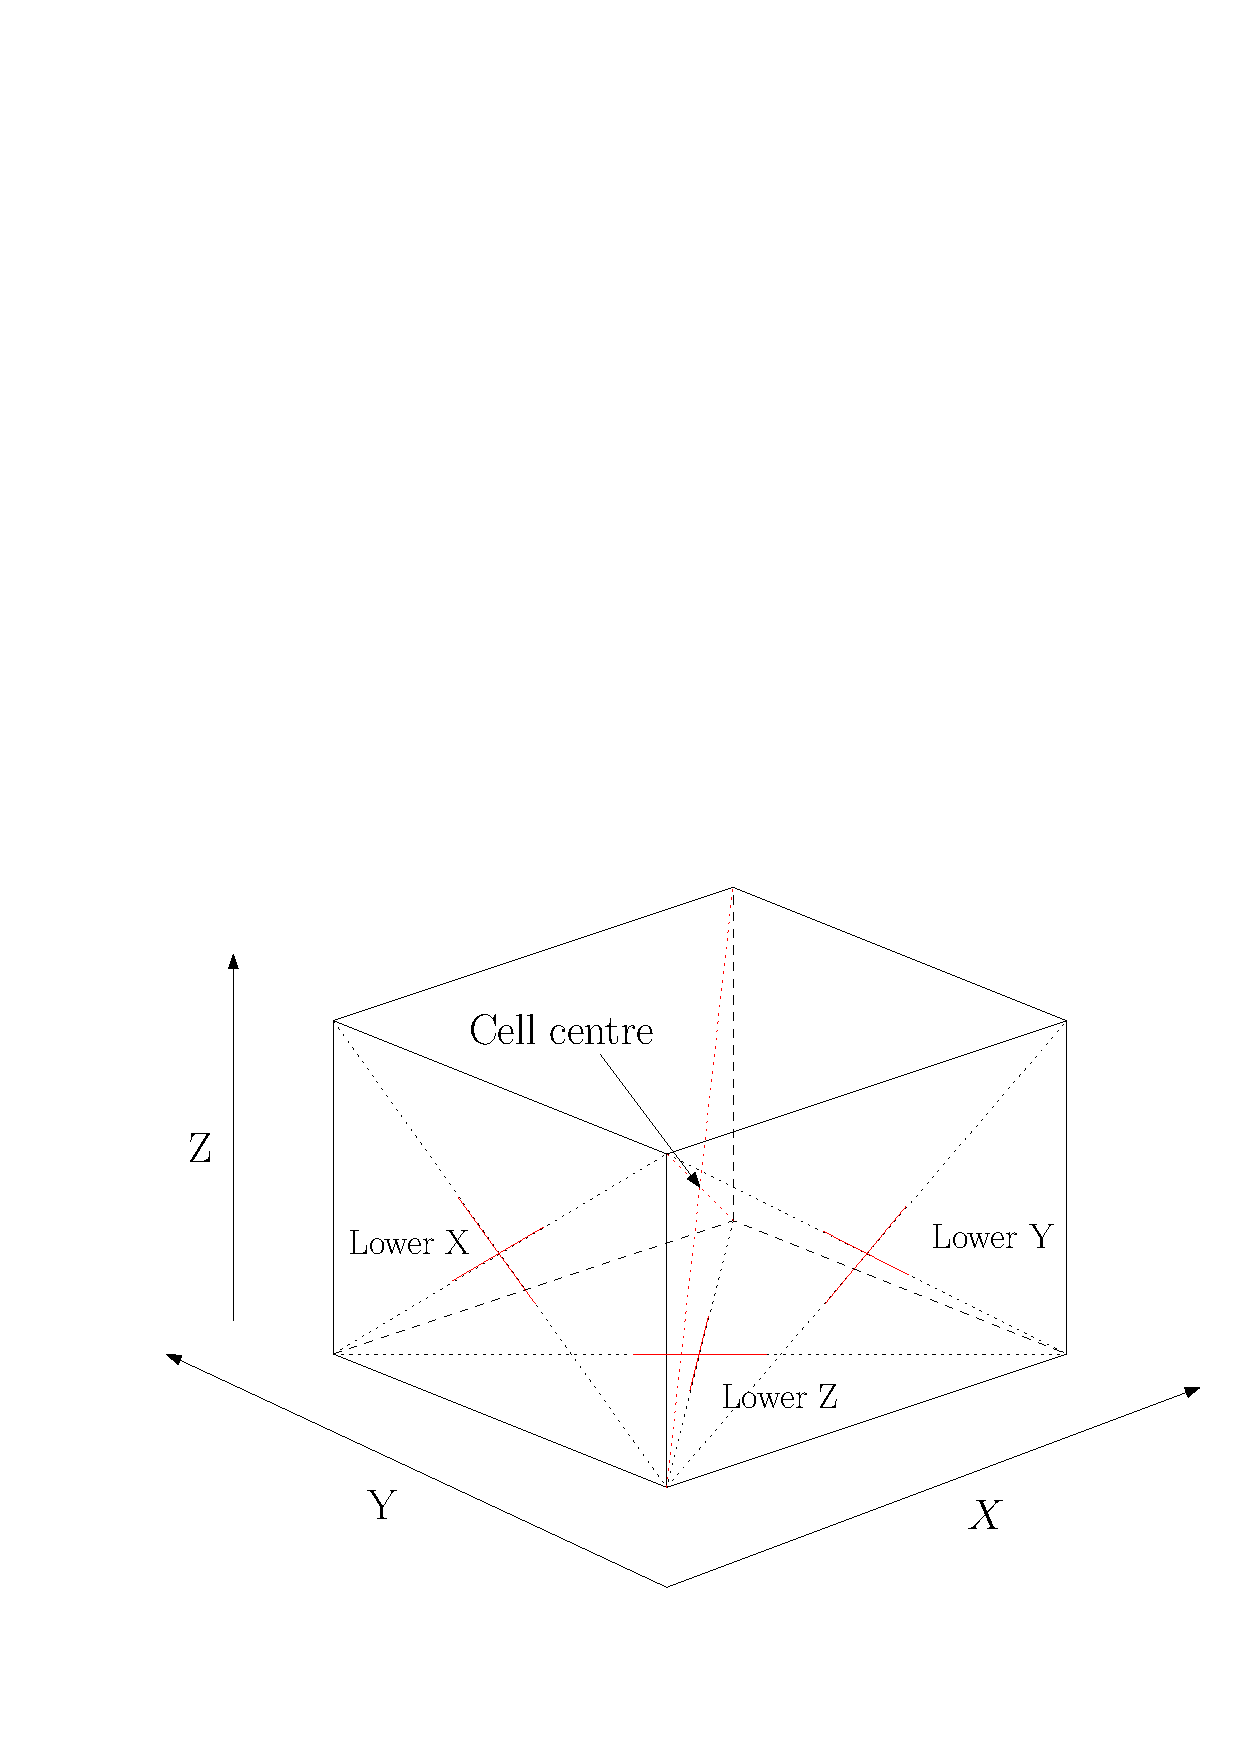
\includegraphics[width=0.4\paperwidth,
keepaspectratio]{figs/stagLocations.pdf}
\caption{Locations in a grid cell where quantities may be defined.}
%
\label{fig:stagLocations}
%
\end{figure}
%
To specify the location of a variable, use the method
%
\lstinline!setLocation()!
%
 with one of the locations
%
\lstinline!CELL\_CENTRE!, \lstinline!CELL\_XLOW!, \lstinline!CELL\_YLOW!, or
\lstinline!CELL\_ZLOW!
%
.

\note{If setting the location of an evolving variable, this should be done {\bf
    before} the call to
%
\lstinline!bout\_solve! or \lstinline!SOLVE\_FOR!
%
}

\noindent The key lines in the {\bf test-staggered} example which specify the
locations of the evolving variables are
%
\begin{lstlisting}
Field3D n, v;

int physics_init(bool restart) {
  v.setLocation(CELL_YLOW); // Staggered relative to n
  SOLVE_FOR2(n, v);
  ...
\end{lstlisting}
%
which makes the velocity
%
\lstinline!v!
%
 staggered to the lower side of the cell in Y, whilst the density $n$ remains
 cell centred.

Arithmetic operations between staggered quantities are handled by interpolating
them to the same location according to the algorithm in
figure~\ref{fig:stagArith}.
%
\begin{figure}[htbp!]
\centering 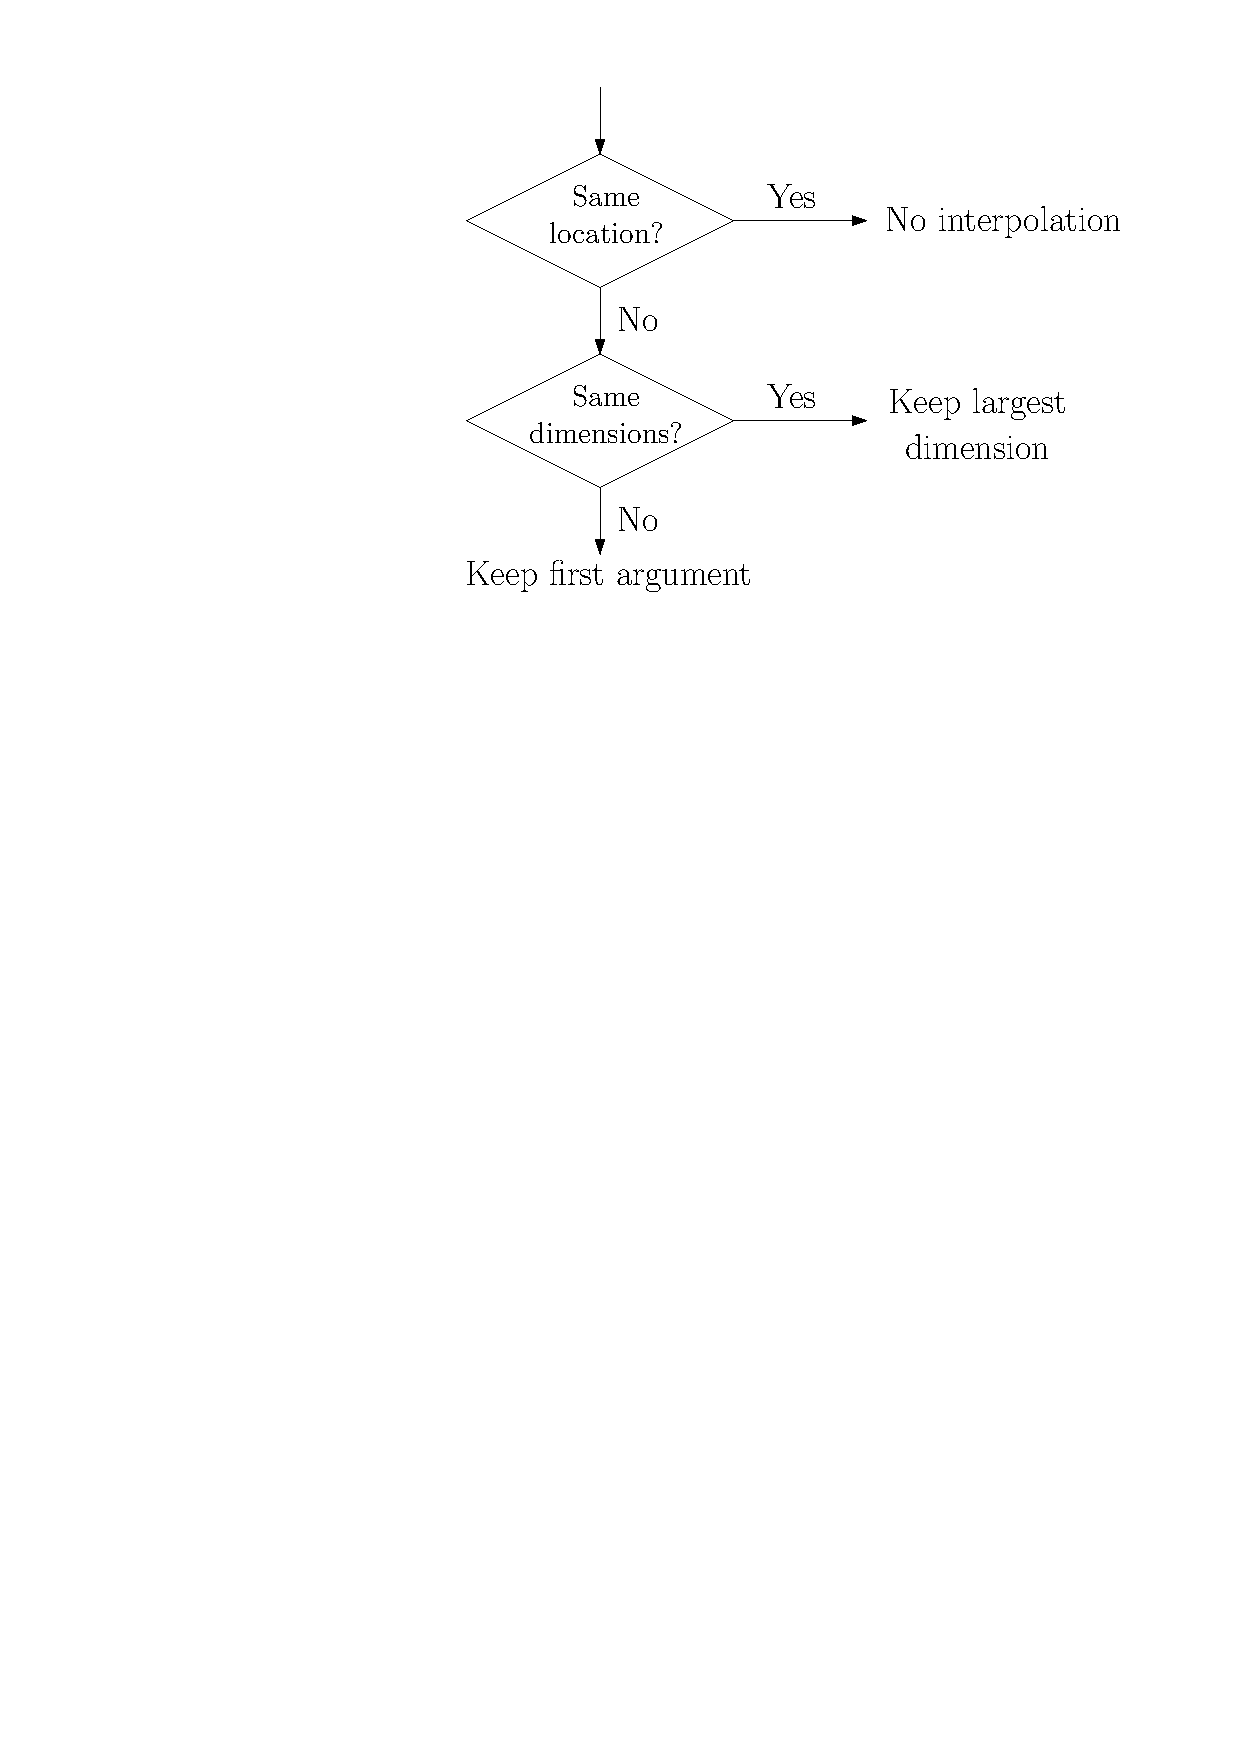
\includegraphics[width=0.4\paperwidth,
keepaspectratio]{figs/stagArith.pdf}
\caption{How the cell location of an arithmetic operation (\code{+,-,*,/,\pow}) is decided}
%
\label{fig:stagArith}
%
\end{figure}
%
If performing an operation between variables defined at two different
locations, the order of the variables matter: the result will be defined at the
locations of the {\bf left} variable. For example,
%
\lstinline!n*v! would be \lstinline!CELL_CENTRE! because this is the location
of \lstinline!n!
%
, whilst
%
\lstinline!v*n! would be \lstinline!CELL_YLOW!
%
. Relying on this behaviour could lead to trouble, to make your code clearer
it's probably best to use the interpolation routines. Include the header file
%
\begin{lstlisting}
#include <interpolation.hxx>
\end{lstlisting}
%
then use the
%
\lstinline!interp_to(field, location)! function. Using this,
\lstinline!interp_to(n, CELL_YLOW)*v!
%
would be
%
\lstinline!CELL_YLOW! as \lstinline!n!
%
 would be interpolated.

Differential operators by default return fields which are defined at the same
location as their inputs, so here
%
\lstinline!Grad_par(v)! would be  \lstinline!CELL_YLOW!
%
. If this is not what is wanted, give the location of the result as an
additional argument:
%
\lstinline!Grad_par(v, CELL_CENTRE)!
%
 uses staggered differencing to produce a result which is defined at the cell
 centres. As with the arithmetic operators, if you ask for the result to be
 staggered in a different direction from the input then the differencing will
 be to cell centre and then be interpolated. For example
%
\lstinline!Grad_par(v, CELL_XLOW)! would first perform staggered differencing
from \lstinline!CELL_YLOW!
%
to get a result at
%
\lstinline!CELL_CENTRE!, and then interpolate the result to
\lstinline!CELL_XLOW!
%
.

Advection operators which take two arguments return a result which is defined
at the location of the field being advected. For example
%
\lstinline!Vpar_Grad_par(v, f)!
%
 calculates $v \nabla_{||} f$ and returns a result at the same location as
%
\lstinline!f!. If \lstinline!v! and \lstinline!f!
%
 are defined at the same locations then centred differencing is used, if one is
 centred and the other staggered then staggered differencing is used, and if
 both are staggered to different locations then the behaviour is less well
 defined (don't do it).  As with other differential operators, the required
 location of the result can be given as an optional argument.

\note{There are subtleties with boundary conditions when staggering variables.
The test-staggered example manually applies a boundary condition to make the
width of the boundary wider}





\section{Advanced methods}
%
\label{sec:precon}
%
This section describes the more advanced methods which can be used to speed up
simulations using implicit time stepping schemes. At the time of writing (Dec
'12), they can be used with either the SUNDIALS CVODE or PETSc solvers.



\subsection{Global field gather / scatter}
%
In BOUT++ each processor performs calculations on a sub-set of the mesh, and
communicates with other processors primarily through exchange of guard cells
(the
%
\lstinline!mesh->commmunicate!
%
 function).  If you need to gather data from the entire mesh onto a single
 processor, then this can be done using either 2D or 3D
%
\lstinline!GlobalFields!
%
.

First include the header file
%
\begin{lstlisting}
#include <bout/globalfield.hxx>
\end{lstlisting}
%
which defines both
%
\lstinline!GlobalField2D! and \lstinline!GlobalField3D!
%
. To create a 3D global field, pass it the mesh pointer:
%
\begin{lstlisting}
  GlobalField3D g3d(mesh);
\end{lstlisting}
%
By default all data will be gathered onto processor 0. To change this, specify
which processor the data should go to as the second input
%
\begin{lstlisting}
  GlobalField3D g3d(mesh, processor);
\end{lstlisting}
%
Gather and scatter methods are defined:
%
\begin{lstlisting}
  Field3D localData;
  // Set local data to some value

  g3d.gather(localData);  // Gathers all data onto one processor

  localData = g3d.scatter(); // Scatter data back
\end{lstlisting}
%
{\bf Note:} Boundary guard cells are {\bf not} handled by the scatter step, as
this would mean handling branch-cuts etc. To obtain valid data in the guard and
Y boundary cells, you will need to communicate and set Y boundaries.

{\bf Note:} Gather and Scatter are global operations, so all processors must
call these functions.

Once data has been gathered, it can be used on one processor. To check if the
data is available, call the method
%
\lstinline!dataIsLocal()!, which will return \lstinline!true!
%
 only on one processor
%
\begin{lstlisting}
  if(g3d.dataIsLocal()) {
    // Data is available on this processor

  }
\end{lstlisting}
%
The sizes of the global array are available through
%
\lstinline!xSize()!, \lstinline!ySize()! and \lstinline!zSize()!
%
methods. The data itself can be accessed indirectly using
%
\lstinline!(x,y,z)!
%
 operators:
%
\begin{lstlisting}
  for(int x=0; x<g3d.xSize(); x++)
    for(int y=0; y<g3d.ySize(); y++)
      for(int z=0; z<g3d.zSize(); z++)
        output.write("Value at (%d,%d,%d) is %e\n",
        x,y,z,
        g3d(x,y,z) );
\end{lstlisting}
%
or by getting a pointer to the underlying data, which is stored as a 1D array:
%
\begin{lstlisting}
  BoutReal *data = g3d.getData();
  nx = g3d.xSize();
  ny = g3d.ySize();
  nz = g3d.zSize();

  data[x*ny*nz + y*nz + z]; // Value at g3d(x,y,z)
\end{lstlisting}
%
See the example \file{examples/test-globalfield} for more examples.





\section{Testing}
%
Two types of tests are currently used in BOUT++ to catch bugs as early as
possible: Unit tests, which check a small piece of the code separately, and a
test suite which runs the entire code on a short problem.
%
\index{Unit tests}
%
Unit tests can be run using the \file{src/unit\_tests} Python script. This
searches through the directories looking for an executable script called
\file{unit\_test}, runs them, and collates the results. Not many tests are
currently available as much of the code is too tightly coupled. If done
correctly, the unit tests should describe and check the behavior of each part
of the code, and hopefully the number of these will increase over time.
%
\index{Test suite}
%
The test suite is in the \file{examples} directory, and is run using the
\file{test\_suite} python script. At the top of this file is a list of the
subdirectories to run (e.g. \file{test-io}, \file{test-laplace}, and
\file{interchange-instability}). In each of those subdirectories the script
\file{runtest} is executed, and the return value used to determine if the test
passed or failed.

All tests should be short, otherwise it discourages people from running the
tests before committing changes. A few minutes or less on a typical desktop,
and ideally only a few seconds. If you have a large simulation which you want
to stop anyone breaking, find starting parameters which are as sensitive as
possible so that the simulation can be run quickly.



\subsection{Method of Manufactured Solutions}
%
The Method of Manufactured solutions (MMS) is a rigorous way to check that a
numerical algorithm is implemented correctly. A known solution is specified
(manufactured), and it is possible to check that the code output converges to
this solution at the expected rate.

To enable testing by MMS, switch an input option ``mms'' to true:
%
\begin{lstlisting}
[solver]
mms = true
\end{lstlisting}
%
This will have the following effect:
%
\begin{enumerate}
\item For each evolving variable, the solution will be used to initialise and
    to calculate the error
\end{enumerate}
%



\subsection{Choosing manufactured solutions}
%
Manufactured solutions must be continuous and have continuous derivatives.
Common mistakes:
%
\begin{itemize}
\item Don't use terms multiplying coordinates together e.g. \texttt{x * z} or
    \texttt{y * z}. These are not periodic in $y$ and/or $z$, so will give
    strange answers and usually no convergence. Instead use \texttt{x * sin(z)}
    or similar, which are periodic.
\end{itemize}
%



\subsection{Timing}
%
\label{sec:timerclass}
%
\index{Timer}
%
To time parts of the code, and calculate the percentage of time spent in
communications, file I/O, etc. there is the
%
\lstinline!Timer!
%
 class defined in \file{include/bout/sys/timer.hxx}. To use it, just create a
%
\lstinline!Timer!
%
object at the beginning of the function you want to time:
%
\begin{lstlisting}
#include <bout/sys/timer.hxx>

void someFunction() {
  Timer timer("test")
  ...
}
\end{lstlisting}
%
Creating the object starts the timer, and since the object is destroyed when
the function returns (since it goes out of scope) the destructor stops the
timer.
%
\begin{lstlisting}
class Timer {
public:
  Timer();
  Timer(const std::string &label);
  ~Timer();

  double getTime();
  double resetTime();
};
\end{lstlisting}
%
The empty constructor is equivalent to setting
%
\lstinline!label = ""!
%
.  Constructors call a private function
%
\lstinline!getInfo()!
%
, which looks up the
%
\lstinline!timer_info!
%
 structure corresponding to the label in a
%
\lstinline!map<string, timer_info*>!
%
. If no such structure exists, then one is created. This structure is defined
as:
%
\begin{lstlisting}
struct timer_info {
  double time;    ///< Total time
  bool running;   ///< Is the timer currently running?
  double started; ///< Start time
};
\end{lstlisting}
%
Since each timer can only have one entry in the map, creating two timers with
the same label at the same time will lead to trouble.  Hence this code is {\bf
not} thread-safe.

The member functions
%
\lstinline!getTime()! and \lstinline!resetTime()!
%
both return the current time. Whereas
%
\lstinline!getTime()!
%
 only returns the time without modifying the timer,
%
\lstinline!resetTime()!
%
 also resets the timer to zero.

If you don't have the object, you can still get and reset the time using static
methods:
%
\begin{lstlisting}
double Timer::getTime(const std::string &label);
double Timer::resetTime(const std::string &label);
\end{lstlisting}
%
These look up the
%
\lstinline!timer_info!
%
 structure, and perform the same task as their non-static namesakes. These
 functions are used by the monitor function in \file{bout++.cxx} to print the
 percentage timing information.





\section{Examples}
%
\label{sec:examples}
%
The code and input files in the \texttt{examples/} subdirectory are for
research, demonstrating BOUT++, and to check for broken functionality. Some
proper unit tests have been implemented, but this is something which needs
improving. The examples which were published in
\cite{Dudson2009,dudson-2008-arxiv} were \texttt{drift-instability},
\texttt{interchange-instability} and \texttt{orszag-tang}.



\subsection{advect1d}
%
The model in \texttt{gas\_compress.cxx} solves the compressible gas dynamics
equations for the density $n$, velocity $\mathbf{V}$, and pressure $P$:



\subsection{drift-instability}
%
The physics code \texttt{2fluid.cxx} implements a set of reduced Braginskii
2-fluid equations, similar to those solved by the original BOUT code.  This
evolves 6 variables: Density, electron and ion temperatures, parallel ion
velocity, parallel current density and vorticity.

Input grid files are the same as the original BOUT code, but the output format
is different.

%
\begin{figure}[htbp!]
\centering \subfigure[Growth rate]{
%
\label{fig:drift_imag}
%
  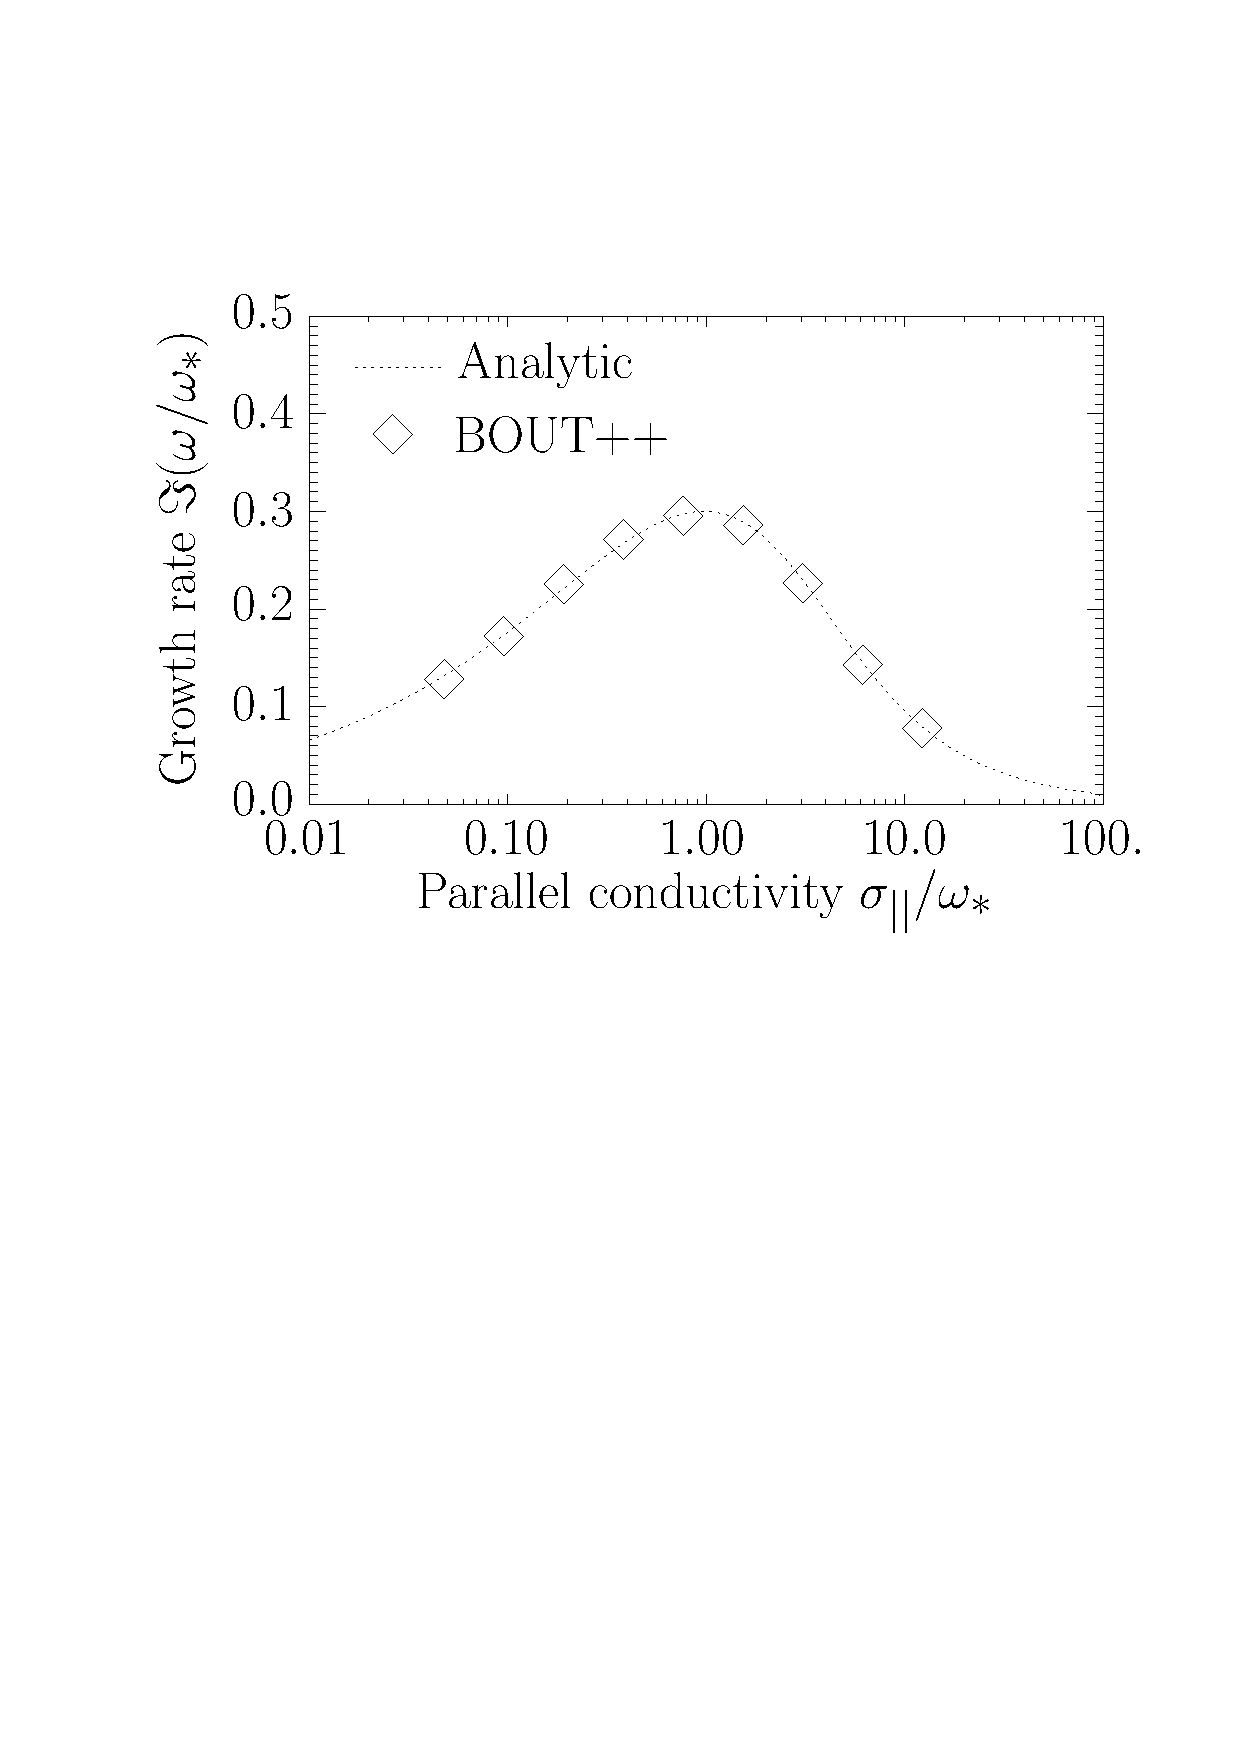
\includegraphics[scale=0.35]{figs/drift_growth.pdf} } \subfigure[Real
  Frequency]{
%
\label{fig:drift_real}
%
  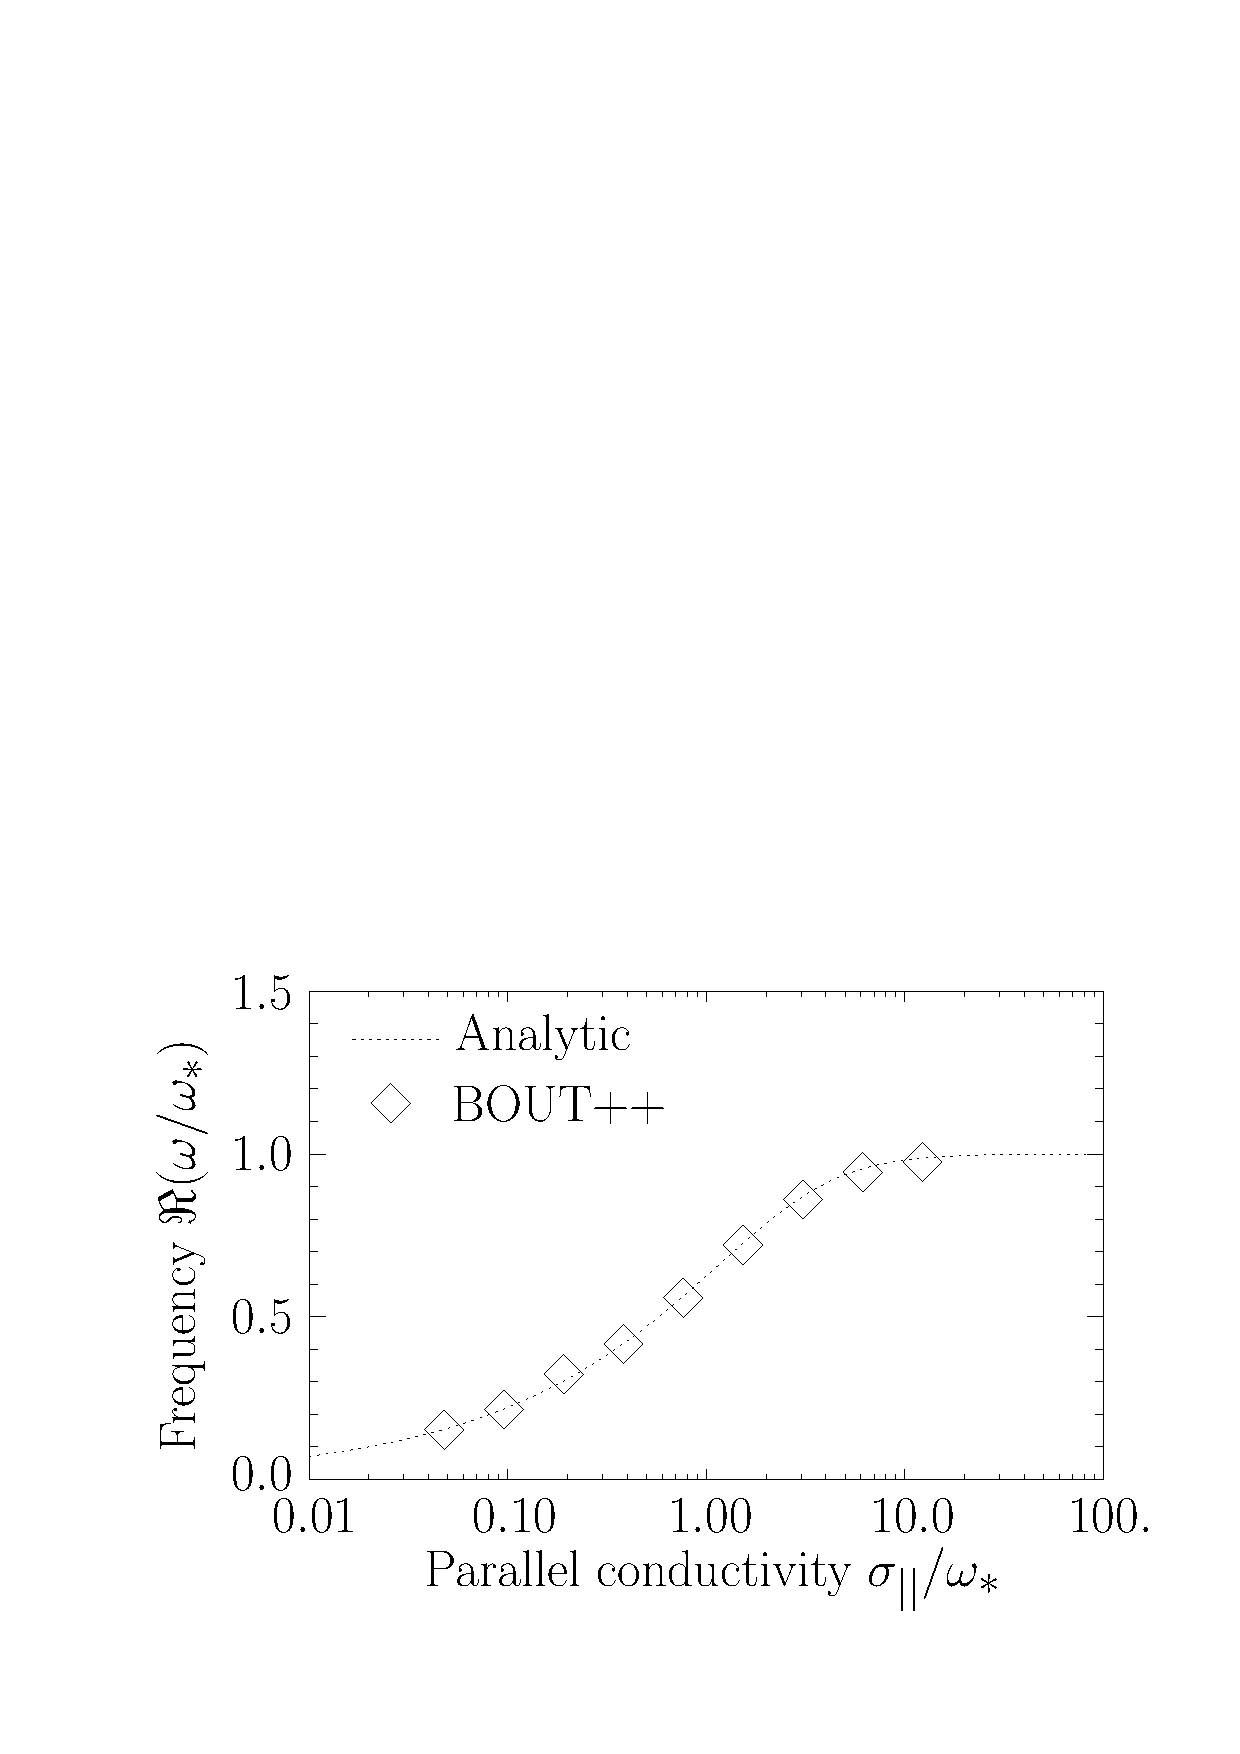
\includegraphics[scale=0.35]{figs/drift_freq.pdf} }
\caption{Resistive Drift wave instability test. Dashed lines are analytic results, diamonds from BOUT++ simulations}
%
\label{fig:drift_test}
%
\end{figure}
%



\subsection{em-drift}
%



\subsection{gyro-gem}
%



\subsection{interchange-instability}
%
\begin{figure}[htb!]
\centering 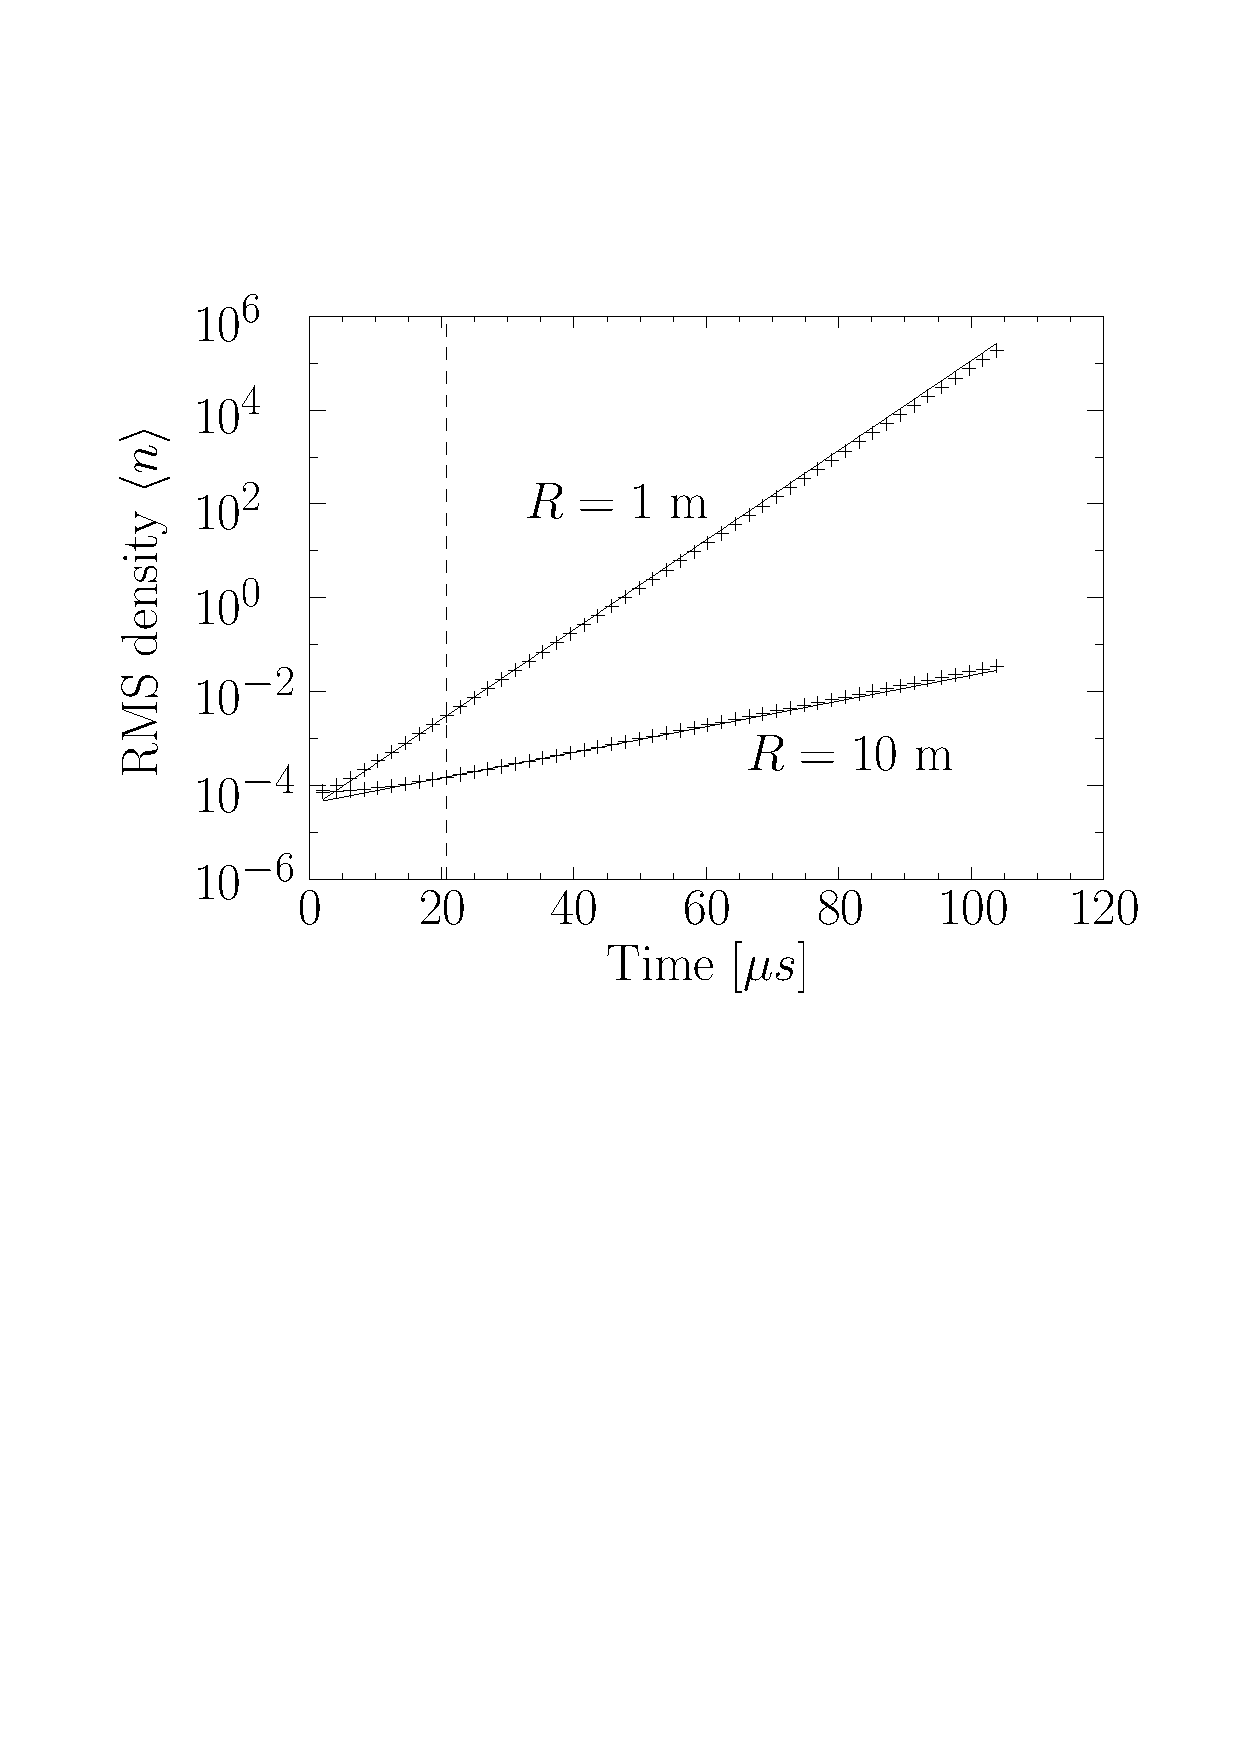
\includegraphics[scale=0.4]{figs/interchange_inst_test.pdf}
\caption{Interchange instability test. Solid lines are from analytic theory, symbols from BOUT++ simulations, and the RMS
density is averaged over $z$. Vertical dashed line marks the reference point,
where analytic and simulation results are set equal}
%
\label{fig:profiles}
%
\end{figure}
%



\subsection{jorek-compare}
%



\subsection{lapd-drift}
%



\subsection{orszag-tang}
%
The file \texttt{mhd.cxx} solves the full MHD equations for the full values
(perturbation + initial), whilst the file \texttt{mhd\_perturb.cxx} solves for
a perturbation about the equilibrium.



\subsection{shear-alfven-wave}
%



\subsection{sod-shock}
%
\begin{figure}[h]
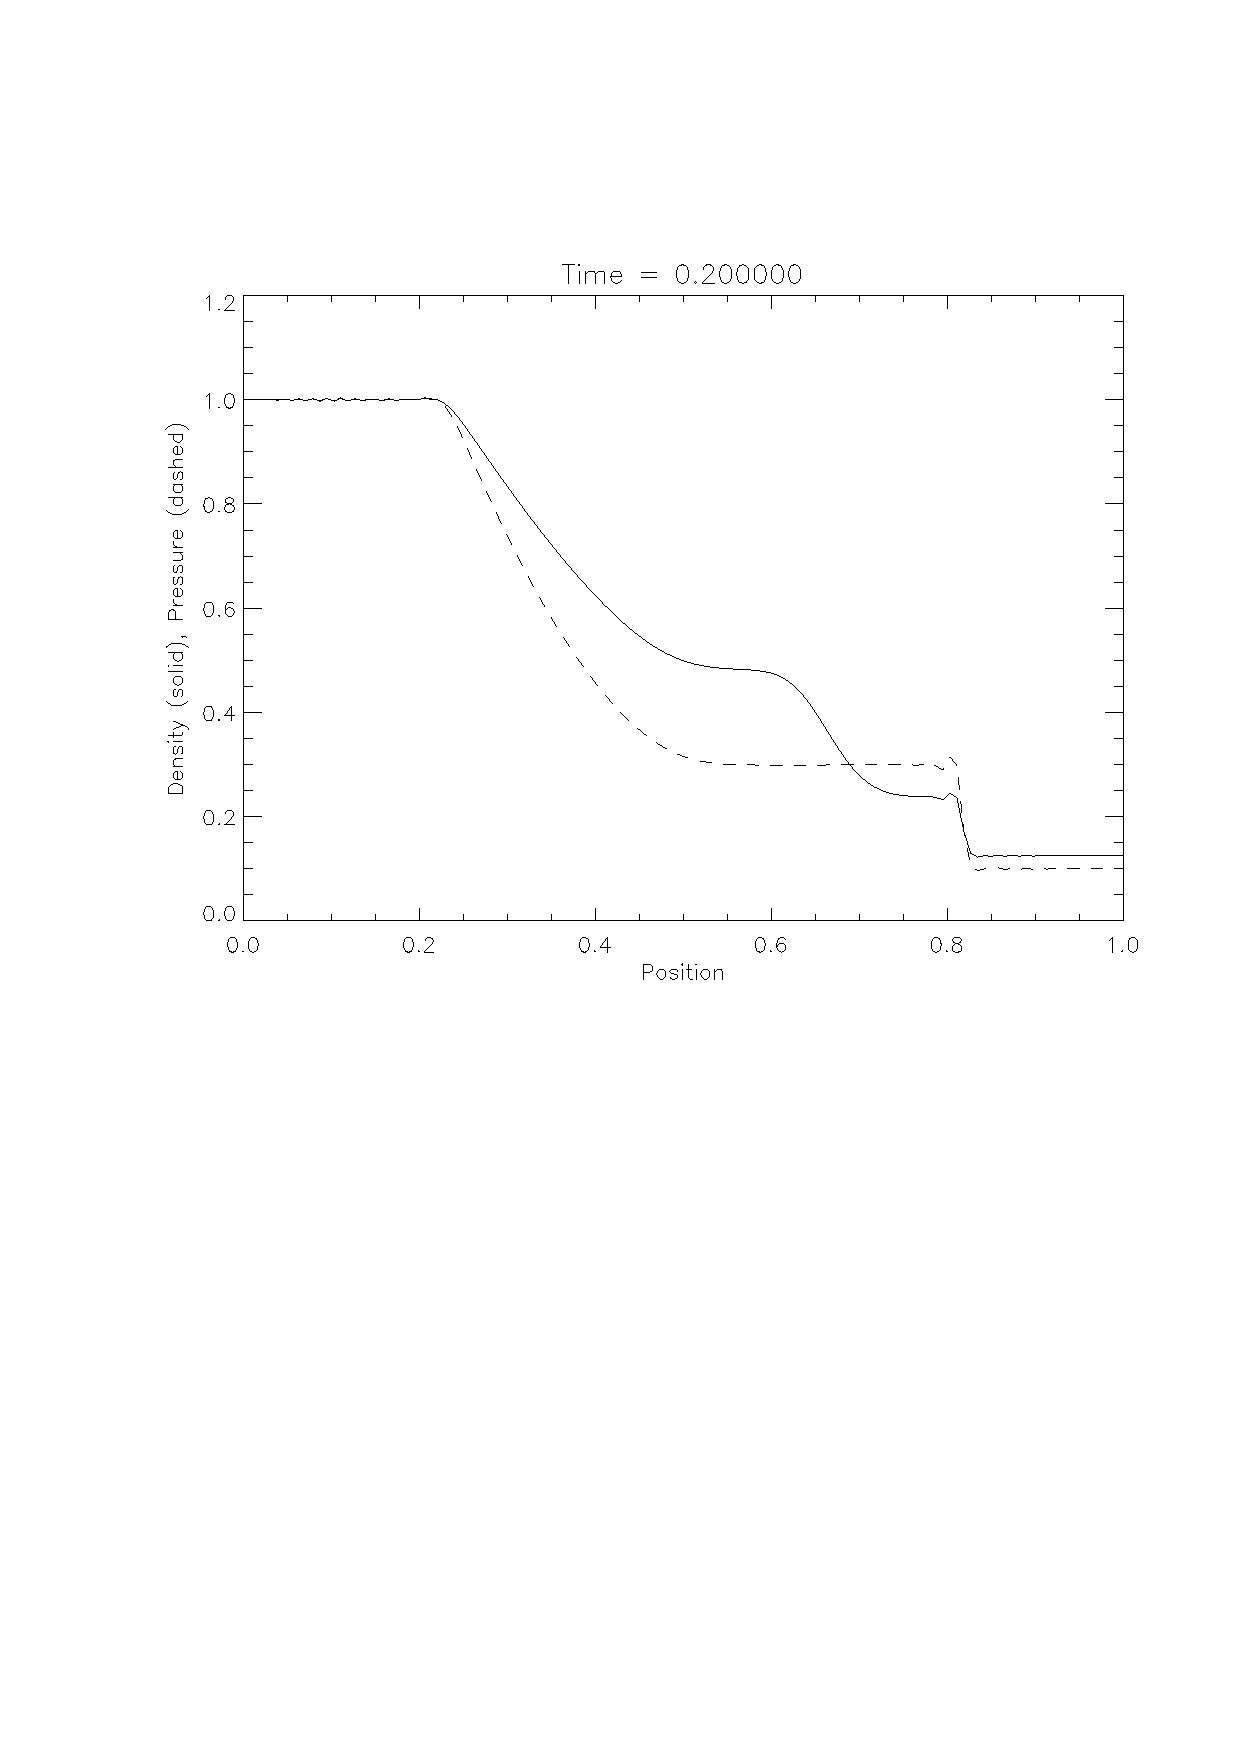
\includegraphics[width=0.48\textwidth, keepaspectratio]{figs/sod_result.pdf}
\caption{Sod shock-tube problem for testing shock-handling methods}
\end{figure}
%



\subsection{uedge-benchmark}
%





\section{Notes}
%



\subsection{Compile options}
%
Compiling with \code{-DCHECK} enables a lot of checks of operations performed
by the field objects. This is very useful for debugging a code, and can be
omitted once bugs have been removed.

For (sometimes) more useful error messages, there is the \code{-DTRACK} option.
This keeps track of the names of variables and includes these in error
messages.



\subsection{Adaptive grids}
%
Two types of adaptive grids can be used in BOUT++: Moving meshes, and changing
resolution.


\subsubsection{Moving meshes}
%
During either the initialisation, or the simulation itself, the metric tensors
can be modified. This could be used to make the coordinate system
time-dependent. Since currently the metric tensors are 2D fields, this would
only allow axisymmetric motion. Changing the tensors to be 3D objects is
however possible with fairly small modification to the code.

Whenever one of the metrics $g^{ij}$ are changed, a call to \code{geometry()}
must be made.


\subsubsection{Changing resolution}
%
\note{Not implemented yet - this just for discussion}

Since all 2D and 3D fields/vectors are located internally in global lists, the
resolution of the grid can be changed when required by interpolation. {\bf This
requires a new, more efficient implementation of the Fields classes}.

\bibliography{references} \bibliographystyle{unsrt}

\appendix





\section{Machine-specific installation}
%
\label{apx:machineinstructions}
%



\subsection{Archer}
%
As of 30th April 2014, the following configuration should work
%
\begin{verbatim}
> module swap PrgEnv-cray PrgEnv-gnu/5.1.29
> module load fftw
> module load netcdf/4.1.3
\end{verbatim}
%





\section{Installing PACT}
%
\label{apx:pact}
%
\index{PACT}
%
There are two ways to install PACT, and usually one of them will work on a
given system.



\subsection{Self-extracting package}
%
This is probably the easiest method (when it works). Download one of the
``Executable UNIX distribution files'' from the PACT website and run:
%
\begin{verbatim}
./pact07_07_18-src -sl -i $HOME/local/
\end{verbatim}
%
The ``-sl'' flag tells it to generate shared libraries. If you don't plan on
using IDL to read/write PDB files, then you can omit this. The ``-i
\$HOME/local/'' tells PACT to install in your home directory/local.

If this script fails, you will usually have to resort to either trying to
understand DSYS, or going with the second method below.



\subsection{PACT source distribution}
%
The second method is to use a .tar.gz PACT source file. Here the version used
is \texttt{pact-2.1.0.tar.gz}.

%
\begin{verbatim}
 ~/ $ cd install
 ~/install/ $ tar -xzvf pact-2.1.0.tar.gz
 ~/install/ $ cd pact-2.1.0/
 ~/install/pact-2.1.0/ $ ./configure --prefix=$HOME/local --enable-shared
\end{verbatim}
%
\note{On Franklin, PACT will compile without the --enable-shared option, but
not with it. This is OK if you just want to run BOUT++, but the shared
libraries are needed for reading the results into IDL (the PDB2IDL library)}

At this point, the installation may fail with the following error:
%
\begin{verbatim}
configure: WARNING: yacc is a symbolic link to bison
configure: WARNING: bison is not a supported type of yacc
configure: error: No working yacc found
\end{verbatim}
%
If this happens, you need to first install Berkeley Yacc into your home
directory
%
\begin{verbatim}
 ~/install/ $ ls
byacc.tar.gz       netcdf-tar -xzvf byacc.tar.gz4.0.1.tar.gz  pact-2.1.0.tar.gz
fftw-3.2.1.tar.gz  pact-2.1.0           sundials-2.4.0.tar.gz

 ~/install/ $ tar -xzvf byacc.tar.gz
 ~/install/ $ cd byacc-20080826/
 ~/install/byacc-20080826/ $ ./configure --prefix=$HOME/local
 ~/install/byacc-20080826/ $ gmake
 ~/install/byacc-20080826/ $ mkdir ~/local/bin
 ~/install/byacc-20080826/ $ cp yacc ~/local/bin/
\end{verbatim}
%
NB: We're copying the yacc executable manually because ``gmake install''
doesn't seem to work, and the fix which works for PACT (see later) doesn't work
here.

Add this directory to your path:
%
\begin{verbatim}
 ~/install/byacc-20080826/ $ setenv PATH $HOME/local/bin:$PATH
\end{verbatim}
%
You can check that this has worked by running ``which yacc'', which should then
print your home directory /local/bin/yacc.  You could also add this to your
.profile startup scripts. Now go back to PACT:
%
\begin{verbatim}
 ~/install/byacc-20080826/ $ cd ../pact-2.1.0
 ~/install/pact-2.1.0/ $ ./configure --prefix=$HOME/local --enable-shared
 ~/install/pact-2.1.0/ $ gmake
 ~/install/pact-2.1.0/ $ gmake install
\end{verbatim}
%
The last step may fail with a strange error message like:
%
\begin{verbatim}
    The current directory must be set to the ITT directory.
    Change the default to the ITT directory and re-run
    this script.
\end{verbatim}
%
This happens when the wrong ``install'' is being used. Check by running:
%
\begin{verbatim}
 ~/install/byacc-20080826/ $ which install
\end{verbatim}
%
This should print ``/usr/bin/install'', but if not then run
%
\begin{verbatim}
 ~/install/byacc-20080826/ $ ln -s /usr/bin/install ~/local/bin/
 ~/install/pact-2.1.0/ $ ./configure --prefix=$HOME/local
 ~/install/pact-2.1.0/ $ gmake
 ~/install/pact-2.1.0/ $ gmake install
\end{verbatim}
%
NOTE: configure needs to be run again after messing with install.

This should now install PACT into your local directory.





\section{Compiling and running under AIX}
%
Most development and running of BOUT++ is done under Linux, with the occasional
FreeBSD and OSX.  The configuration scripts are therefore heavily tested on
these architectures. IBM's POWER architecture however runs AIX, which has some
crucial differences which make compiling a pain.

%
\begin{itemize}
\item Under Linux/BSD, it's usual for a Fortran routine \code{foo} to appear
    under C as \code{foo\_}, whilst under AIX the name is unchanged
\item MPI compiler scripts are usually given the names \code{mpicc} and
  either \code{mpiCC} or \code{mpicxx}. AIX uses \code{mpcc} and \code{mpCC}.
\item Like BSD, the \code{make} command isn't compatible with GNU make,
  so you have to run \code{gmake} to compile everything.
\item The POWER architecture is big-endian, different to the little endian
  Intel and AMD chips. This can cause problems with binary file formats.
\end{itemize}
%



\subsection{SUNDIALS}
%
To compile SUNDIALS, use
%
\begin{verbatim}
$ export CC=cc
$ export CXX=xlC
$ export F77=xlf
$ export OBJECT_MODE=64
$ ./configure --prefix=$HOME/local/ --with-mpicc=mpcc --with-mpif77=mpxlf CFLAGS=-maix64
\end{verbatim}
%
You may get an error message like:
%
\begin{verbatim}
make: Not a recognized flag: w
\end{verbatim}
%
This is because the AIX \code{make} is being used, rather than \code{gmake}.
The easiest way to fix this is to make a link to \code{gmake} in your local bin
directory:
%
\begin{verbatim}
$ ln -s /usr/bin/gmake $HOME/local/bin/make
\end{verbatim}
%
Running \code{which make} should now point to this \code{local/bin/make}, and
if not then you need to make sure that your bin directory appears first in the
\code{PATH}:
%
\begin{verbatim}
export PATH=$HOME/local/bin:$PATH
\end{verbatim}
%
If you see an error like this:
%
\begin{verbatim}
ar: 0707-126 ../../src/sundials/sundials_math.o is not valid with the current object file mode.
        Use the -X option to specify the desired object mode.
\end{verbatim}
%
then you need to set the environment variable \code{OBJECT\_MODE}
%
\begin{verbatim}
export OBJECT_MODE=64
\end{verbatim}
%
Configuring BOUT++, you may get the error:
%
\begin{verbatim}
configure: error: C compiler cannot create executables
\end{verbatim}
%
In that case, you can try using:
%
\begin{verbatim}
./configure CFLAGS="-maix64"
\end{verbatim}
%
When compiling, you may see warnings
%
\begin{verbatim}
xlC_r: 1501-216 (W) command option -64 is not recognized - passed to ld
\end{verbatim}
%
At this point, the main BOUT++ library should compile, and you can try
compiling one of the examples.

%
\begin{verbatim}
ld: 0711-317 ERROR: Undefined symbol: .NcError::NcError(NcError::Behavior)
ld: 0711-317 ERROR: Undefined symbol: .NcFile::is_valid() const
ld: 0711-317 ERROR: Undefined symbol: .NcError::~NcError()
ld: 0711-317 ERROR: Undefined symbol: .NcFile::get_dim(const char*) const
\end{verbatim}
%
This is probably because the NetCDF libraries are 32-bit, whilst BOUT++ has
been compiled as 64-bit.  You can try compiling BOUT++ as 32-bit:
%
\begin{verbatim}
$ export OBJECT_MODE=32
$ ./configure CFLAGS="-maix32"
$ gmake
\end{verbatim}
%
If you still get undefined symbols, then go back to 64-bit, and edit
make.config, replacing \code{-lnetcdf\_c++} with {-lnetcdf64\_c++}, and
\code{-lnetcdf} with {-lnetcdf64}. This can be done by running:
%
\begin{verbatim}
$ sed 's/netcdf/netcdf64/g' make.config > make.config.new
$ mv make.config.new make.config
\end{verbatim}
%





\section{BOUT++ functions (alphabetical)}
%
This is a list of functions which can be called by users writing a physics
module. For a full list of functions, see the Reference manual, DOxygen
documentation, and source code.

%
\begin{itemize}
  \item \texttt{Field = {\bf abs}(Field | Vector)}
  \item \texttt{(Communicator).{\bf{add}}(Field | Vector)} \\ Add a variable to
      a communicator object.
  \item \texttt{{\bf apply\_boundary}(Field. ``name'')}
  \item \texttt{Field = {\bf b0xGrad\_dot\_Grad}(Field, Field, CELL\_LOC)}
  \item \texttt{{\bf bout\_solve}(Field, Field, ``name'')}
  \item \texttt{{\bf bout\_solve}(Vector, Vector, ``name'')}
  \item \texttt{(Communicator).{\bf{clear}}()} \\ Remove all variables from a
      Communicator object
  \item \texttt{Field = {\bf cos}(Field)}
  \item \texttt{Field = {\bf cosh}(Field)}
  \item \texttt{Vector = {\bf Curl}(Vector)}
  \item \texttt{Field = {\bf Delp2}(Field)} \\ $\nabla_\perp^2$ operator
  \item \texttt{Field = {\bf Div}(Vector)} \\
    Divergence of a vector
  \item \texttt{Field = {\bf Div\_par}(Field f)} \\
    Parallel divergence $B_0\mathbf{b}\cdot\nabla\left(f / B_0\right)$
  \item \texttt{{\bf dump.add}(Field, ``name'', 1/0)}
  \item \texttt{Field = {\bf filter}(Field, modenr)}
  \item \texttt{{\bf geometry\_derivs}()} \\ Calculates useful quantities from
      the metric tensor. Call this every time the metric tensor is changed.
  \item \texttt{Vector = {\bf Grad}(Field)}
  \item \texttt{Field = {\bf Grad\_par}(Field)}
  \item \texttt{Field = {\bf Grad2\_par2}(Field)}
  \item \texttt{{\bf grid\_load}(BoutReal, ``name'')} \\ Load a scalar real
      from the grid file
  \item \texttt{{\bf grid\_load2d}(Field2D, ``name'')} \\
    Load a 2D scalar field from the grid file
  \item \texttt{{\bf grid\_load3d}(Field3D, ``name'')} \\
    Load a 3D scalar field from the grid file
  \item \texttt{{\bf invert\_laplace}(Field input, Field output, flags, Field2D *A)}
  \item \texttt{Field = {\bf invert\_parderiv}(Field2D|BoutReal A,
      Field2D|BoutReal B, Field3D r)} \\ Inverts an equation  \code{A*x +
      B*Grad2\_par2(x) = r}
  \item \texttt{Field = {\bf Laplacian}(Field)}
  \item \texttt{Field3D = {\bf low\_pass}(Field3D, max\_modenr)}
  \item \texttt{BoutReal = {\bf max}(Field)}
  \item \texttt{BoutReal = {\bf min}(Field)}
  \item \texttt{{\bf msg\_stack.pop}( |int)} \\ Remove a message from the top
      of the stack. If a message ID is passed, removes all messages back to
      that point.
  \item \texttt{int = {\bf msg\_stack.push}(``format'', ...)} \\
    Put a message onto the stack. Works like \code{printf} (and
    \code{output.write}).
  \item \texttt{{\bf options.get}(``name'', variable, default)} \\
    Get an integer, real or boolean value from the options file.  If not in the
    file, the default value is used. The value used is printed to log file.
  \item \texttt{{\bf options.setSection}(``name'')}
    Set the section name in the input file
  \item \texttt{{\bf output} $< <$ values} \\
    Behaves like cout for stream output
  \item \texttt{{\bf output.write}(``format'', ...)}  \\
    Behaves like printf for formatted output
  \item \texttt{(Communicator).{\bf{receive}}()} \\
    Receive data from other processors. Must be preceded by a \code{send} call.
  \item \texttt{(Communicator).{\bf{run}}()} \\
    Sends and receives data.
  \item \texttt{(Communicator).{\bf{send}}()} \\
    Sends data to other processors (and posts receives). This must be followed
    by a call to \code{receive()} before calling send again, or adding new
    variables.
  \item \texttt{(Field3D)\bf{.setLocation}(CELL\_LOC)}
  \item \texttt{(Field3D)\bf{.ShiftZ}(bool)}
  \item \texttt{Field = {\bf{sin}}(Field)}
  \item \texttt{Field = {\bf{sinh}}(Field)}
  \item \texttt{{\bf solver.setPrecon}(PhysicsPrecon)} \\ Set a preconditioner
      function
  \item \texttt{Field = \bf{sqrt}(Field)}
  \item \texttt{Field = {\bf tan}(Field)}
  \item \texttt{Field = {\bf tanh}(Field)}
  \item \texttt{Field = {\bf V\_dot\_Grad}(Vector v, Field f)} \\ Calculates an
      advection term $\mathbf{v}\cdot\nabla f$
  \item \texttt{Vector = {\bf V\_dot\_Grad}(Vector v, Vector u)} \\
    Advection term $\mathbf{v}\cdot\nabla\mathbf{u}$
  \item \texttt{Field = {\bf Vpar\_Grad\_par}(Field v, Field f)}
  \item \texttt{Field3D = {\bf where}(Field2D test, Field|BoutReal gt0,
      Field|BoutReal lt0)} \\ Chooses between two values, depending on sign of
      \code{test}.
\end{itemize}
%





\section{IDL routines}
%
\label{apx:idl_routines}
%
List of IDL routines available in idllib. There are broadly three categories of
routine:
%
\begin{itemize}
\item Completely general routines which could be useful outside BOUT++ work
  %
  \begin{itemize}
  \item Data plotting and animation: {\bf contour2} and {\bf showdata}
  \item File reading and writing: {\bf file\_open}, {\bf file\_read} etc.
  \item User input and output: {\bf get\_float}, {\bf get\_integer}, {\bf
      get\_yesno} and {\bf str}
  \item FFT routines for integrating, differentiating and filtering: {\bf fft\_integrate}, {\bf fft\_deriv}, {\bf fft\_filter}
  \end{itemize}
%
\item Routines for BOUT++, but not specific to any application
  %
  \begin{itemize}
  \item Modifying restart files: {\bf expand\_restarts}, {\bf scale\_restarts}
      and {\bf split\_restarts}
  \item Processing 3D variables for input grid: {\bf bout3dvar}
  \end{itemize}
%
\item Routines specifically for tokamak simulations
  %
  \begin{itemize}
  \item Reading A- and G-EQDSK format files into IDL: {\bf read\_aeqdsk} and
      {\bf read\_neqdsk}
  \item Plotting results: {\bf polslice}, {\bf plotpolslice}
  \end{itemize}
%
\end{itemize}
%
Here the format is

{\bf name}, arguments, [optional arguments]

%
\begin{itemize}
\item var = {\bf bout3dvar} ( var ) \\ Converts 3D variables to and from
    BOUT++'s Fourier representation which is used for input grids. By default
    converts from [x,y,z] to [x,y,f]
  %
  \begin{itemize}
  \item {\bf /reverse}  Convert from [x,y,f] to [x,y,z]
  \item {\bf nf}=nf Set number of frequencies in the result
  \item {\bf nz}=nz When using /reverse, set number of Z points in the result
  \end{itemize}
%
\item var = {\bf collect}() \\
  Read in data from a set of BOUT++ dump files
  %
  \begin{itemize}
    \item {\bf var} = ``name of variable''
    \item {\bf path} = ``path/to/variable/''
    \item {\bf xind}, {\bf yind}, {\bf zind}, {\bf tind}  = [min, max] index
        pairs
    \item {\bf t\_array} = Output 1D array of times
  \end{itemize}
%
\item {\bf contour2}, data [, x, y] \\
  This is a replacement for the IDL contour which includes a scale color bar.
  %
  \begin{itemize}
  \item {\bf data} can be either 2D (x,y) or 3D (x,y,t). If data is 3D then the
      color is scaled to the entire range.
  \item {\bf x} is an optional 2D (x,y) array of X coordinates
  \item {\bf y} is an optional 2D (x,y) array of Y coordinates
  \item {\bf t}=t is a time index for 3D data
  \item {\bf nlev}=nlev
  \item {\bf centre}=centre  Make zero the middle of the color range (white if
      redblue)
  \item {\bf redblue}=redblue  Use a blue-white-red color scheme
  \item {\bf revcolor}=revcolor  Reverse color scheme
  \end{itemize}
%
\item {\bf expand\_restarts}, newz \\
  Increases the number of Z points in restart files. Together with
  scale\_restarts and split\_restarts, this makes it easier to modify a linear
  simulation as a start for non-linear runs.
  %
  \begin{itemize}
  \item {\bf newz} is the new value of NZ
  \item {\bf path}=path      Input path
  \item {\bf output}=output  Output path
  \item {\bf format}=format  File extension of output
  \end{itemize}
%
\item result = {\bf fft\_deriv} ( var1d ) \\
  Calculates the derivative of a variable on a periodic domain.
\item result = {\bf fft\_filter} (var, nf)
  Fourier filter a variable on a periodic domain. Arguments are a 1D variable
  and the number of Fourier components to keep
\item result = {\bf fft\_integrate} ( var1d )
  Integrates a variable on a periodic domain.
  %
  \begin{itemize}
  \item {\bf loop}=loop  The loop integral is returned in this variable
  \end{itemize}
%
\item {\bf file\_close}, handle \\
  Close a file opened using file\_open()
\item list = {\bf file\_list} ( handle ) \\
  Return a list of variable names in the file
\item integer = {\bf file\_ndims} ( handle , ``variable'' ) \\
  Get the number of dimensions of a variable
\item handle = {\bf file\_open} ( ``file'' ) \\
  Open a PDB or NetCDF file. File type is inferred from file name
  %
  \begin{itemize}
    \item {\bf /write}  Open file for writing (default is read only)
    \item {\bf /create} Create a new file, over-writing if already exists
  \end{itemize}
%
\item var = {\bf file\_read} ( handle, ``variable'' )
  %
  \begin{itemize}
    \item {\bf inds} = [xmin, xmax, ymin, ymax, ... ]
  \end{itemize}
%
\item float = {\bf get\_float} ( ``prompt'' ) \\
  Ask the user for a float, using the given prompt
\item integer = {\bf get\_integer} ( ``prompt'' ) \\
  Ask the user for an integer
\item integer = {\bf get\_yesno} ( ``prompt'' ) \\
  Ask for a yes (1) or no (0) answer
\item result = {\bf gmres} ( x0, operator, b ) \\
  General Minimal Residual (GMRES)
   %
   \begin{itemize}
    \item {\bf x0} is the starting guess at the solution
    \item {\bf operator}
    \item {\bf b}
   \end{itemize}
%
   Optional arguments
   %
   \begin{itemize}
   \item {\bf restart}=restart
   \item {\bf max\_iter}=max\_iter
   \item {\bf tol}=tol
   \item {\bf stats}=stats
   \item {\bf show}=show
   \item {\bf output}=output
   \end{itemize}
%
\item result = {\bf int\_func} ( [x,] f ) \\
  Integrate a function, always using the maximum
  number of grid-points possible for highest accuracy
\item bool = {\bf is\_pow2} ( value ) \\
  Returns 1 (true) if the given number is a power of 2, 0 (false) otherwise
\item {\bf plotpolslice}, var3d, grid \\
  Takes a slice through a field-aligned tokamak domain, showing a poloidal cross-section.
  %
  \begin{itemize}
  \item {\bf var3d} is a 3D (x,y,z) variable to plot. Needs all of the points to work properly.
  \item {\bf grid} is a structure from importing a grid file
  \end{itemize}
%
  Optional arguments:
  %
  \begin{itemize}
  \item {\bf period}=period
  \item {\bf zangle}=zangle
  \item {\bf nlev}=nlev
  \item {\bf yr}=yr
  \item {\bf profile}=profile
  \item {\bf output}=output
  \item {\bf lines}=lines
  \item {\bf linecol}=linecol
  \item {\bf filter}=filter
  \end{itemize}
%
\item {\bf polslice}, data, gridfile \\
  Plots a 2D poloidal contour for single or double-null configurations, including color bar.
  %
  \begin{itemize}
    \item {\bf xstart}=xstart  X index where the data begins. Useful if only part of the domain has been collected
    \item {\bf ystart}=ystart  Y index where data begins
  \end{itemize}
%
\item struct = {\bf read\_aeqdsk} ( "filename" ) \\
  Reads an A-EQDSK file. Format is specified here:
  \url{https://fusion.gat.com/THEORY/efit/a_eqdsk.html}
\item struct = {\bf read\_neqdsk} ( "filename" ) \\
  Reads in an 'neqdsk' or G-EQDSK formatted tokamak equilibrium file.
  Format of G-EQDSK file is specified here:
  \url{https://fusion.gat.com/THEORY/efit/g_eqdsk.html}
\item stringarray = {\bf regex\_extract} ( line, pattern ) \\
  Extract all matches to Regular Expression pattern contained in line.
  Useful for extracting numbers from FORTRAN-formatted text files.
  %
  \begin{itemize}
  \item {\bf line} Input string
  \item {\bf pattern} Regular expression pattern to match
  \item {\bf nmatch}=nmatch
  \end{itemize}
%
\item var = {\bf reverse\_inds} ( var ) \\
  Reverse array indices e.g. \code{arr[t,z,y,x] -> arr[x,y,z,t]}. Works on up to 5 dimensional variables
\item {\bf safe\_colors} \\
  Sets the color table to useful values for plotting.
  %
  \begin{itemize}
  \item {\bf /first}   Sets the first 10 colors to specific values, otherwise sets last 7
  \end{itemize}
%
\item {\bf scale\_restarts}, factor
  %
  \begin{itemize}
  \item {\bf path}=path  Path to the restart files (default is current directory '.')
  \item {\bf format}=format  Specify what the file format is, otherwise goes on the file name
  \end{itemize}
%
\item {\bf showdata}, data \\
  Display animations of 1D,2D and 3D data. Defaults:
  %
  \begin{itemize}
  \item 2D data   Animate a line plot
  \item 3D data   Animate a surface plot
  \item 4D data   Animate a poloidal cross-section (tokamaks only)
  \end{itemize}
%
  Optional arguments:
  %
  \begin{itemize}
  \item {\bf /addsym}   For 2D data (1D plots), add symbols to mark data points
  \item {\bf az}=angle       Rotate surface plots
  \item {\bf /bw} Make contour plots grey scale
  \item {\bf chars}=size character size
  \item {\bf /contour}  For 3D input, show color contour plot
  \item {\bf delay}=time     Time delay between plots (default 0.2 seconds)
  \item {\bf /noscale}       By default, all plots are on the same scale.
    This changes the scale for each plot's range
  \item {\bf profile}=array  Background profile. Data is 3D: profile is 1D (X).
    Data is 4D -> profile is 2D (X,Y)
  \item {\bf yr}=[min,max]   Y range
  \end{itemize}
%
\item result = {\bf sign} ( var ) \\
  This returns +1 if the variable is $> 0$, -1 otherwise
\item {\bf spectrum}
\item {\bf split\_restarts}, [nxpe], nype \\
  split restart files between a different number of processors
  %
  \begin{itemize}
  \item {\bf nxpe} is an optional argument giving the number of
    processors in the X direction
  \item {\bf nype} is the number of processors in the Y direction
  \item {\bf path}=path      Input path
  \item {\bf output}=output  Output path
  \item {\bf format}=format  File extension of output
  \end{itemize}
%
\item string = {\bf str} ( value ) \\
  Convert a value to a string with whitespace trimmed. Arrays are
  converted to a comma-separated list in brackets.
\item result = {\bf zfamp} ( var4d )\\
  Given a 4D variable [x,y,z,t], returns the Fourier amplitudes in [x,y,f,t]
\item var = {\bf zshift} ( var, shift ) \\
  Shifts a variable in the Z direction, useful for mapping between field-aligned and orthogonal
  coordinates.
  %
  \begin{itemize}
  \item {\bf period}=period  How many domains fit in $2\pi$. Default is 1 (full torus)
  \end{itemize}
%
\end{itemize}
%





\section{Python routines (alphabetical)}
%
\label{apx:py_routines}
%



\subsection{boututils}
%
\begin{itemize}
\item
%
\lstinline!class Datafile!
%
 provides a convenient way to read and write NetCDF or HDF5 files. There are
 many different NetCDF libraries available for Python, so this class tries to
 provide a consistent interface to many of them, as well as to h5py.
\item
%
\lstinline!deriv()!
%
\item
%
\lstinline!determineNumberOfCPUs()!
%
\item
%
\lstinline!file_import()!
%
 reads the contents of a NetCDF file into a dictionary
\item
%
\lstinline!integrate()!
%
\item
%
\lstinline!launch()!
%
\item
%
\lstinline!linear_regression()!
%
\end{itemize}
%



\subsection{boutdata}
%
\begin{itemize}
\item
%
\lstinline!collect()!
%
 provides an interface to read BOUT++ data outputs, returning NumPy arrays of data.
  It deals with the processor layout, working out which file contains each part of the domain.
  %
  \begin{lstlisting}
    from boutdata import collect

    t = collect("t_array")  # Collect the time values
  \end{lstlisting}
%
\item
%
\lstinline!pol_slice()!
%
 takes a 3 or 4-D data set for a toroidal equilibrium, and calculates a slice
  through it at fixed toroidal angle.
\item
%
\lstinline!gen_surface()!
%
 is a generator for iterating over flux surfaces
\end{itemize}
%



\subsection{bout\_runners}
%
\label{sec:bout_runners}
%
\lstinline!bout_runners!
%
contains classes which gives an alternative way of running BOUT++ simulations
either normally using the class
%
\lstinline!basic_runner!
%
, or on a cluster through a generated Portable Batch System
(PBS) script using the child class
%
\lstinline!PBS_runner!
%
. Examples can be found in \file{examples/bout\_runners\_example/}.

\note{
%
\lstinline!bout_runners!
%
 is currently only tested on clusters using
%
\lstinline!TORQUE!
%
}

%
\lstinline!bout_runners!
%
 is especially useful if one needs to make several runs with only small
changes in the options (which is normally written in \file{BOUT.inp} or in the
command-line), as is the case when performing a parameter scan, or when
performing a MMS test.

Instead of making several runs with several different input files with only
small changes in the option, one can with
%
\lstinline!bout_runners!
%
 specify the
changes as member data of an instance of the appropriate
%
\lstinline!bout_runners!
%
 class. One way to do this is to write a \emph{driver}
in the same directory as the executable. The \emph{driver} is just a
python script which imports
%
\lstinline!bout_runners!
%
, creates an instance, specifies the
running option as member data of that instance and finally calls the
member function
%
\lstinline!self.execute_runs()!
%
.

In addition, the
%
\lstinline!bout_runners!
%
provides a way to run any python post-processing script after finished
simulations (as long as it accept at least one parameter containing the folder
name(s) of the run(s)). If the simulations have been performed using the
%
\lstinline!PBS_runner!
%
, the post-processing function will be submitted to the cluster (although it is
possible to submit it to a different queue, using a different amount of nodes
etc.).

When the function
%
\lstinline!self.execute_runs()!
%
 is executed, a folder structure like
the one presented in figure~\ref{fig:folder_tree} is created.
\file{BOUT.inp} is copied to the folder of execution, where the
\file{BOUT.*.dmp} files are stored. Secondly a list of combination of the
options specified in the driver is made. Eventually unset options are obtained
from \file{BOUT.inp} or given a default value if the option is nowhere to be
found.
%
\begin{landscape}
\thispagestyle{empty}
 \vspace*{2cm}
 %
 \begin{figure}[htbp!]
 \hspace*{-4cm}
\centering
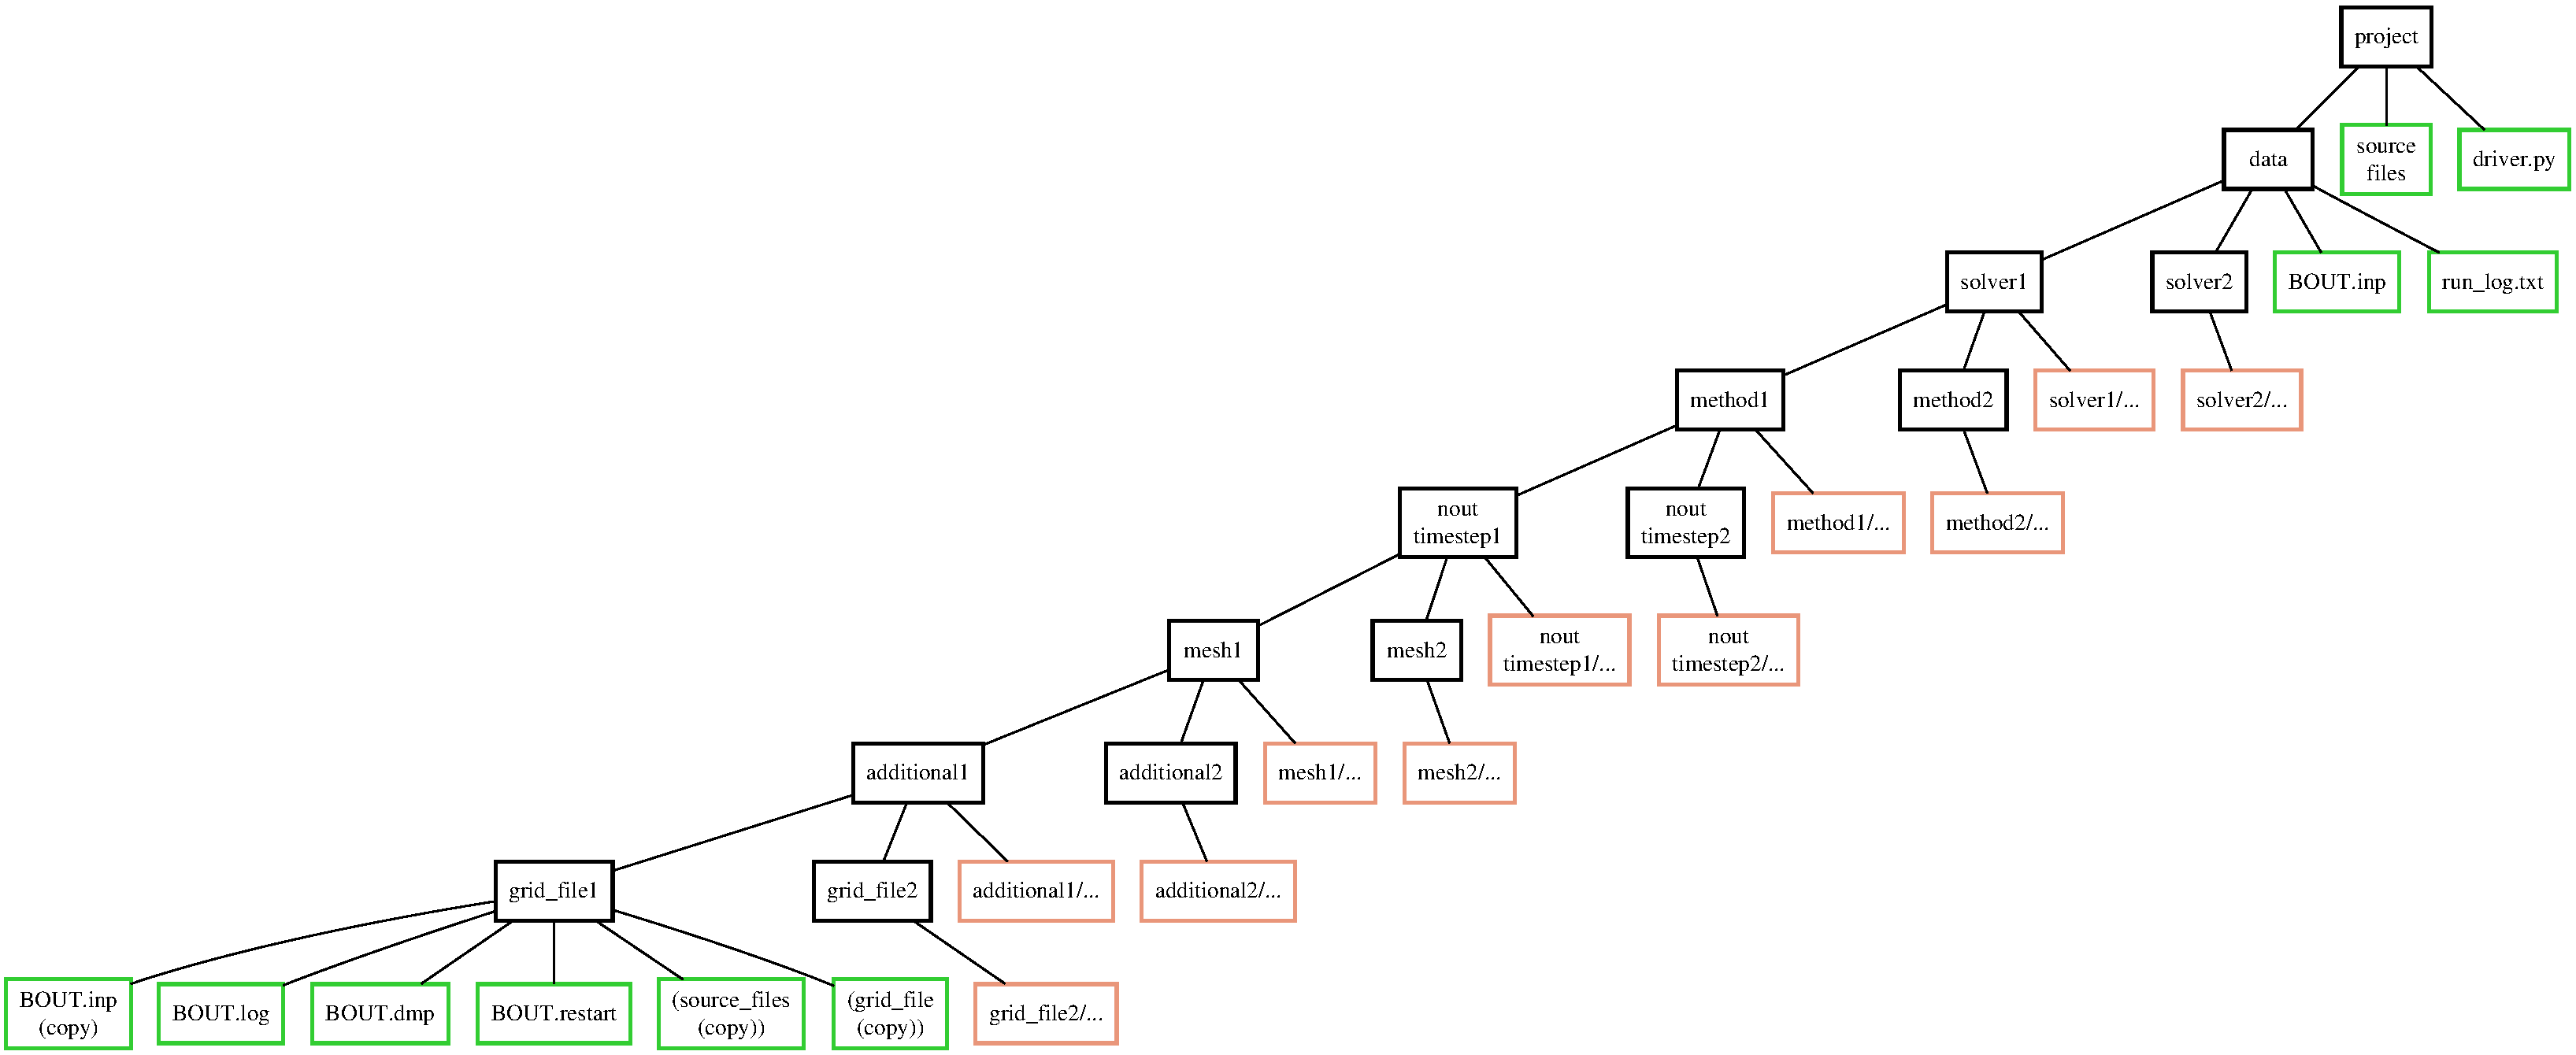
\includegraphics[width=1.35\hsize]{figs/folder_tree.pdf}
\caption{Longest possible folder tree made by the
%
\lstinline!self.execute_runs()!
%
function.}
%
\label{fig:folder_tree}
%
\end{figure}
%
\end{landscape}


\printindex

\end{document}
%

